\chapter{Numerical Results}
\label{chapter 6}
In this chapter, we present the results generated by our numerical solvers based on projection methods: Alg 1, Alg 2 and Alg 3, as well as the Gauge method. We investigate each method's accuracy through numerical tests and visual simulations.

\section*{Numerical validation of Projection methods}
\section{Accuracy test}
There are many ways to test the accuracy of numerical schemes. One of the most popular way is to compare the numerical solutions generated through computer simulations with analytical solutions. By calculating the error with appropriate norms (e.g. $L_1,\,L_2$ and $L_\infty$) this method provides precise measure on error and convergence rate. In case where analytical solutions are not known or difficult to implement, people often use bench mark results. These results are not the analytical solutions to the test problem, rather they are numerical solutions generated in fine grids that are widely accepted in literature. For instance, the lid driven cavity problem is such a simple test problem which shows turbulent flow patterns. We will give a qualitative illustration of the classic cavity problem in this chapter too.

For the main part of this chapter because we are aiming to conduct accuracy and convergence test of projection methods, hence we consider two simple 2-D flow problems where analytic solutions do exist. This reveals more fundamental properties and error behaviours for the projection schemes.\\

\subsection{Forced flow}
The test problem is a forced flow example where the fluid is confined in a square domain $\Omega = [-1,1] \times [-1,1]$ and initially remains stationary. The flow is initiated by an external driving force. This is one of the simplest settings to consider slip/no-slip boundary conditions. In this case an homogeneous boundary condition (no - slip) is imposed on the four sides of the domain \\
($\partial \Omega:$ West: $x = -1$, East: $x=1$, South: $y = -1$, North: $y=1$).\\

The analytical solution satisfies:
\begin{equation}
\begin{cases}
u = \pi\sin(t)\sin(2\pi y)\sin^2(\pi x) \text{   in $\Omega$} \\
v = - \pi \sin(t)\sin(2\pi x)\sin^2(\pi y) \text{   in $\Omega$} \\
p = \sin(t)\cos(\pi x)\sin(\pi y)  \text{   in $\Omega$}  \\
u_0 = u(t=0,x,y)  \text{   in $\Omega$}  \\
v_0 = v(t=0,x,y)  \text{   in $\Omega$}  \\
\end{cases}
\end{equation}
with homogeneous Dirichlet boundary condition:
\begin{equation*}
u(t, x=\pm 1, y) = v(t, x,y= \pm 1) = 0
\end{equation*}

It is augmented with a forcing term: $f = \partial_t\,\textbf{u} - \dfrac{1}{R}\nabla^2 \textbf{u} + \nabla p$ to make the above ``solutions" valid. For simplicity we take the Reynolds number ($R$) to be 1. By substituting our analytical solutions into $f$ we find the forcing term is:
\begin{equation}
f = 
\begin{cases}
fx = \pi\cos(t)\sin(2\pi y)\sin^2(\pi x) -  2 \pi^3\sin(t)\sin(2\pi y)\,(\cos(2\pi x) - 2\sin^2(\pi x)) \\
\,\,\,\,\,\,\,- \, \pi\sin(t)\sin(\pi y)\sin(\pi x) \text{   in $\Omega$} \\
fy = - \pi\cos(t)\sin(2\pi x)\sin^2(\pi y) - 2\pi^3\sin(t)\sin(2\pi x)\,(2\sin^2(\pi y) - \cos(2\pi y)) \\
\,\,\,\,\,\,\,+ \, \pi\sin(t)\cos(\pi x)\cos(\pi y)  \text{   in $\Omega$}  \\
\end{cases}
\end{equation}

The Courant-Friedrichs-Lewy condition (CFL) number is given as: $CFL = U\,(\Delta t/\Delta x + \Delta t/\Delta y)$ (CFL for 2D problems) where $U = \pi$ is the absolute bound for velocity. We want the CFL number to be below one to ensure stability. However too small CFL number will decrease the efficiency because the numerical solver would take a longer time to run to incorporate small time stepping. Hence we have chosen the optimal CFL number to be 0.5. This is also a commonly used value \cite{brown2001accurate}.

The actual error $e_h$ is consisted of both spatial and temporal error and $h$ is just an index to indicate the grid size (e.g. a 120 $\times$ 120 grid).\\
In our purpose of testing the temporal error behaviour, we want the temporal error to dominate and thus we can assume the following simplified error relation:
\begin{equation}
e_h = \Delta t^p
\end{equation}
where $p$ is the convergence rate or order of accuracy (don't be confused with pressure) and in our case we want $p=2$.\\

The error $e_h$ is simply calculated by taking the difference between numerical and analytical solutions point-wisely. It is important to compare the solutions only under the same conditions, for instance sane grid sizes and end of time... Comparing solutions at different time would of course cause strange error behaviours!\\

By taking the logarithm on both side of the equation above we see that the logarithm of error in time has a linear relationship with the logarithm of time stepping ($\Delta t$). Thus the slope of the log error function should be the convergence rate $p$.
\begin{equation}
\log_{10} (e_h) = p\log_{10} (\Delta t)
\end{equation}
Base 10 is used for simplicity, other bases including 2 and natural exponential works the same.\\

The strategy is follows: with the error of a coarse grid denoted as $e_h$. We half the spatial stepping ($\Delta x$) or equivalently double the grid size (e.g. from 15 $\times$ 15 to 30 $\times$ 30). Denoting the error of the finer grid as $e_{h_{1/2}}$. The time stepping mean while is also halved. Then we look at how the error decreases. If our numerical scheme is second order accurate then the error should decrease by a factor of 4 going from the coarser grid to finer grid.\\

A Log-Log plot of the error function is then generated and the convergence rate is finally extracted as the slope of the log error function.\\

It is important to specify the error norm. As noted by many researchers that different norms could generated different convergence rates! \cite{pyo2005normal,guermond2004error}\\
In our analysis 3 commonly used norms were implemented: $L_1,\,L_2$ and $L_\infty$. Each could reveal certain aspect of error behaviour. By combing the results using these 3 norms, a comprehensive analysis of convergence rate can be obtained.\\

We take the normalised $L_1$ norm and it is defined as:
\begin{equation}
||\,e^n\,||_{L_1} = \dfrac{1}{M}\,\sum^M_{m=0}\,|e^n_m|
\end{equation} 
where $e^n$ is the error field measured at time iteration $n$ and $M$ is the dimension or size of the error field. For instance a $15 \times 15$ grid corresponds to $M = 15^2$.\\

similarly we define the $L_2$ norm to be:
\begin{equation}
||\,e^n\,||_{L_2} = \left(\dfrac{1}{M^2}\,\sum^M_{m=0}\,|e^n_m|^2\right)^{1/2} = \dfrac{1}{M}\left(\sum^M_{m=0}\,|e^n_m|^2\right)^{1/2}
\end{equation}

and $L_\infty$:
\begin{equation}
||\,e^n\,||_{L_\infty} = \max_{\,\,\,0 \leq m \leq M\,\,\,}\,|e^n_m|
\end{equation}

To achieve optimal results, there are a number of things that need to be considered. \\
First, since we are aiming to investigate the temporal error and hence we need to use fine grids (small spatial stepping: $\Delta x <<1$) to ensure the spatial error is negligible. Formally we want: $\Delta x^2 << \dfrac{1}{R}\Delta t$. Hence we have run the solvers up to a grid size of $240 \times 240$ and also $480 \times 480$ sometimes. Higher grid numbers are also possible but takes very long time to compute, which would decrease the efficiency. For completeness we have also included the results for small to moderate grids. Overall we have maximum 6 data points corresponding to grid size of 15, 30, 60, 120, 240 and 480.\\

Second, care must also be taken to the pressure gradient along the boundary. We need to make sure the normal pressure gradient is non-zero along the boundary so that the accuracy performance can be distinguished between projection method Alg 1 and Alg 2. Fortunately, for our forced flow solutions, the normal pressure gradient is non-zero along the North and South boundaries ($y = \pm 1$) (whereas it is zero along the other two boundaries).\\

With the above conditions all satisfied, we can now finally test our numerical solutions! As for a start, we run the simulations at $t = 1$ with the spatial domain: $[-1,1]^2$ and homogeneous Dirichlet boundary conditions imposed on velocities.\\

The exact and numerical solutions are summarised in Figure 6.1. The numerical solutions are computed by Alg 2 with grid size: $60 \times 60$ and $CFL = 0.5$. The numerical solutions seem to do a good job in approximating the true solutions. These ``nice" graphs however do not reveal much information about the error behaviours. Hence we need to look at the convergence rates instead.\\

We first compare Alg 1 and Alg 2 results to illustrate the improvement of modified pressure update formula (Equation 3.32 a) with $q = p^{n-1/2}$). The errors for grid size 30 to 120 are summarised in Table 1. In addition the convergence rates for both $U$ and $V$ velocities are highly identical, hence we only report the $U$ component results in the subsequent analysis. It is clear that the velocities in both Alg 1 and Alg 2 show second order convergence rates across all norms whereas in pressure they do not. For Alg 1, $L_1$ and $L_2$ norms show first order convergence rate (1.29 and 1.21 respectively) whereas $L_\infty$ shows an even deteriorated rate of 0.32. The sudden drop in convergence rate in $L_\infty$ indicates the presence of numerical boundary layer, because $L_\infty$ picks up the large errors or singularities better. \\
   For Alg 2, the results in pressure are better, but still not very satisfied. $L_1$ norm shows a close to second order rate of 1.92 whereas $L_2$ shows a decreased rate of about 1.74. The $L_\infty$ then further decreased to only about first order rate (1.14). The degradation of accuracy in $L_\infty$ also indicate the presence of large singularities, whereas $L_1,\,L_2$ tend to smooth them out. The overall magnitude of error is also relatively smaller in Alg 2. Take a look at the pressure error field in Figure 6.2, we found a pronounced numerical boundary layer in Alg 1 corresponding to $y = \pm 1$. Note that the normal gradient of pressure at these two boundaries is $\textbf{n}\cdot \nabla p |_{y = \pm 1} = \mp \pi \sin(t)\,\cos(\pi x) \neq 0$. Hence this indicates clearly the numerical boundary layer is very much formed by the inconsistent normal pressure gradient resulted from the old pressure updated formula used in Alg 1. In Alg 2 the numerical boundary layer seems still exists but reduced to four thinner spikes located at the corners of the domain. In addition, the magnitude of the boundary layer in Alg 2 is also about 4 times smaller. All these observations indicate that the modified pressure update formula in Alg 2 do seem to filter out the spurious mode contained in the intermediate velocity field and auxiliary field better, and hence gives better pressure error convergence. This is consistent with our predications in normal mode analysis and also matches with the findings from other researchers like David, Strikwerda and Shen et al \cite{brown2001accurate, strikwerda1999accuracy, guermond2006overview, guermond2004error}.\\

\begin{table}[H]
  \begin{center}
    \begin{tabular}{| l | c | c c c | r |}
    \hline
    Error in $U$ velocity \\
    \hline
    Alg 1 & Error norm & $30 \times 30$ & $60 \times 60$ & $120 \times 120$ & rates \\
     & $L_1$ & 3.75e-4 & 9.34e-5 & 2.32e-5 & 2.01 \\
     & $L_2$ & 4.66e-4 & 1.16e-4 & 1.88e-5 & 2.0 \\
     & $L_\infty$ & 1.11e-3 & 2.77e-4 & 6.89e-5 & 2.02\\
    \hline
    Alg 2
     & $L_1$ & 3.23e-4 & 8.01e-5 & 1.99e-5 & 2.01 \\
     & $L_2$ & 4.09e-4 & 1.01e-4 & 2.53e-5 & 2.00 \\
     & $L_\infty$ & 9.23e-4 & 2.33e-4 & 5.81e-5 & 2.00\\
    \hline
    \hline
    Error in Pressure\\
    \hline
    Alg 1 & Error norm & $30 \times 30$ & $60 \times 60$ & $120 \times 120$ & rates \\
     & $L_1$ & 6.96e-3 & 1.77e-3 & 7.29e-4 & 1.29 \\
     & $L_2$ & 1.02e-2 & 3.07e-3 & 1.33e-3 & 1.21 \\
     & $L_\infty$ & 6.64e-2 & 3.87-2 & 3.01e-3 & 0.32\\
    \hline
    Alg 2
     & $L_1$ & 1.26e-3 & 2.99e-4 & 8.32e-5 & 1.92 \\
     & $L_2$ & 1.68e-3 & 4.59e-4 & 1.47e-4 & 1.74 \\
     & $L_\infty$ & 9.36e-3 & 6.31e-3 & 3.24e-3 & 1.14\\
	\hline
    \end{tabular}
  \end{center}
  \caption{Error in $U$ velocity and pressure for Alg 1 and Alg 2, cfl = 0.5}
\end{table}

\begin{figure}[H]
	\centering
	\begin{subfigure}[t]{2.5in}
		\centering
		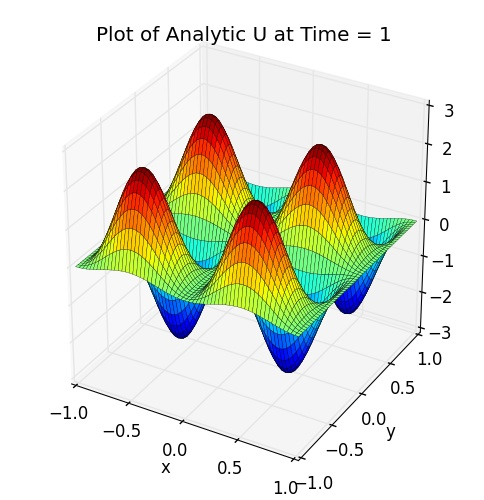
\includegraphics[width=2.5in]{figures/Pm1a_pf2_U_exact_t_1_grid_60 - Copy.jpg}
		\caption{Analytic $U$ velocity at $t=1$}\label{fig:6.1a}		
	\end{subfigure}
	\quad
	\begin{subfigure}[t]{2.5in}
		\centering
		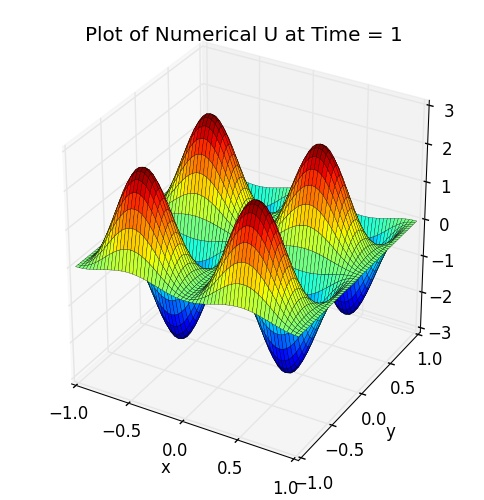
\includegraphics[width=2.5in]{figures/Pm1a_pf2_uf_t_1_grid_60 - Copy.jpg}
		\caption{Numerical $U$ velocity at $t=1$}\label{fig:6.1b}
	\end{subfigure}
	\quad
	\begin{subfigure}[t]{2.5in}
		\centering
		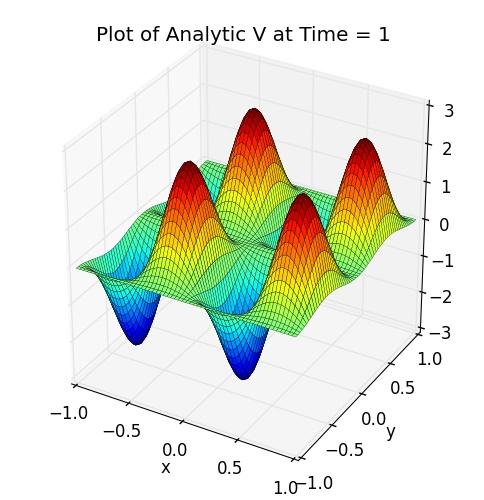
\includegraphics[width=2.5in]{figures/Pm1a_pf2_V_exact_t_1_grid_60 - Copy.jpg}
		\caption{Analytic $V$ velocity at $t=1$}\label{fig:6.1c}
	\end{subfigure}
	\quad
	\begin{subfigure}[t]{2.5in}
		\centering
		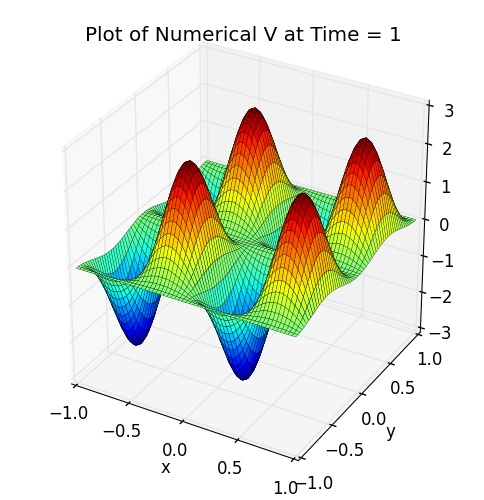
\includegraphics[width=2.5in]{figures/Pm1a_pf2_vf_t_1_grid_60 - Copy.jpg}
		\caption{Numerical $V$ velocity at $t=1$}\label{fig:6.1d}
	\end{subfigure}
	\quad	
	\begin{subfigure}[t]{2.5in}
		\centering
		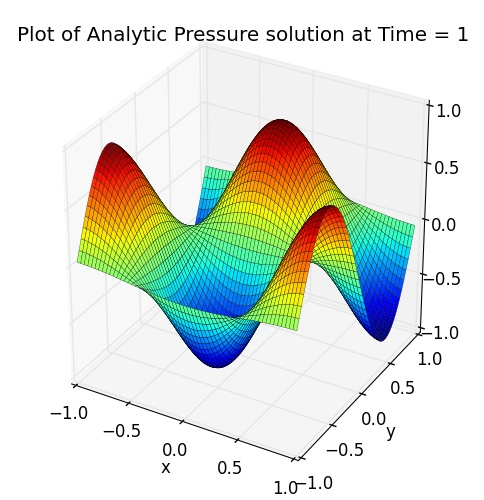
\includegraphics[width=2.5in]{figures/Pm1a_pf2_P_exact_t_1_grid_60 - Copy.jpg}
		\caption{Analytic pressure ($P$) at $t=1$}\label{fig:6.1e}
	\end{subfigure}
	\quad	
	\begin{subfigure}[t]{2.5in}
		\centering
		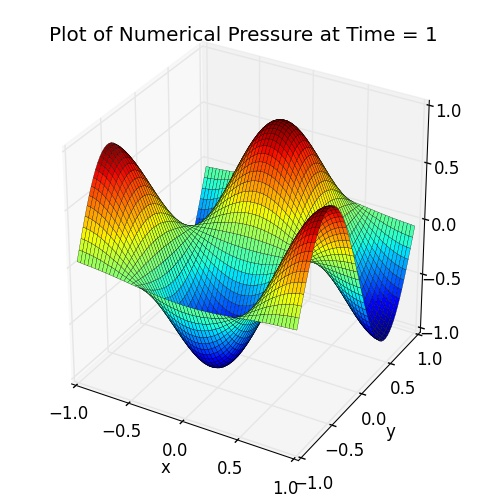
\includegraphics[width=2.5in]{figures/Pm1a_pf2_pf_t_1_grid_60 - Copy.jpg}
		\caption{Numerical pressure ($P$) at $t=1$}\label{fig:6.1f}
	\end{subfigure}
	\caption{Plot of exact and numerical solutions ($U,V,P$) at time $t=1$ on the spatial domain of $[-1,1]^2$ with grid size $60 \times 60$, Alg 2 was used to compute the numerical solutions with $CFL=0.5$}\label{fig:6.1}
\end{figure}

\begin{figure}[H]
	\centering
	\begin{subfigure}[t]{2.5in}
		\centering
		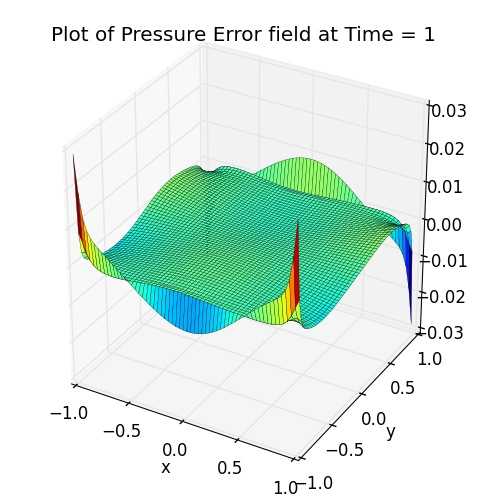
\includegraphics[width=2.5in]{figures/Pm1a_pf2_P_error_t_1_grid_60_cfl_0_1.jpg}
		\caption{Pressure error field for Alg 1 at $t=1$ }\label{fig:6.2a}		
	\end{subfigure}
	\quad
	\begin{subfigure}[t]{2.5in}
		\centering
		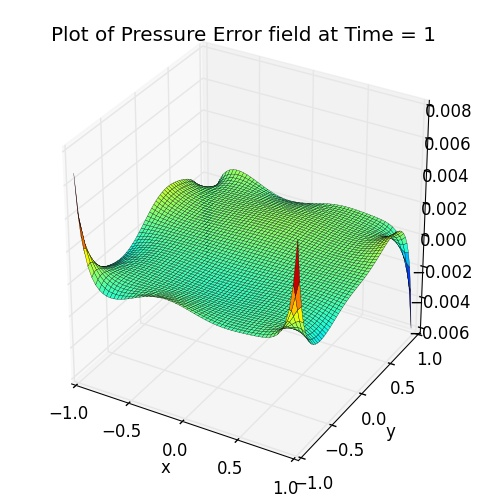
\includegraphics[width=2.5in]{figures/Pm1b_pf2_P_error_t_1_grid_60_cfl_0_1.jpg}
		\caption{Pressure error field for Alg 2 at $t=1$}\label{fig:6.2b}
	\end{subfigure}
	\caption{$3D$ surface plot of pressure error field for Alg 1 and Alg 2 at time $t=1$ on the spatial domain of $[-1,1]^2$ with grid size $60 \times 60$ and $CFL=0.5$}\label{fig:6.2}
\end{figure}

We then compare with the schemes that were all predicated to be second order accurate, namely Alg 2, Alg 3 and Gauge method. The same test problem is used with the same domain ($[-1,1]^2$) and end time to ensure consistency. This time only the convergence in pressure error and divergence of intermediate velocity fields are shown because the convergence in velocities in all methods are consistently second order. We focus more on the error in pressure.\\

The Log-Log plot for errors in pressure are summarised below. We have run the code from $15 \times 15$ up to the $480 \times 480$ the finest. Even finer grids are also able to be calculated by increasing the number of cells, but this is omitted due to the exceedingly long hours take in solving the Poisson equations.\\

Interestingly we observe an outlier at grid size 15 where the pressure error is very large compared to the those at the finer grids. This is observed in all methods for this test problem. This is most likely due to the large spatial error which dominates at such a small grid size. Hence for the sake of reliability, we excluded these data points when computing the convergence rates. The errors after grid 60 reduces consistently and converge asymptotically to the second order reference slope (especially for Alg 3 and Gauge method). This asymptotic convergence behaviour is due to the gradual phasing out of spatial errors dominance at finer and finer grids. This is the most common error behaviour in Projection methods and our results now fully line up with those found in literature \cite{guermond2004error}. \\

Even though Alg 3 and Gauge methods show optimal 2nd order convergence for this test problem, the projection method Alg 1 however shows deprecated convergence especially measured in $L_\infty$. This is because the four spikes in the pressure error plot for Alg 2 before. The pressure error field for Alg 3 and Gauge method shows smooth boundary layers instead. Interestingly the convergence rates in $\nabla \cdot \textbf{u}^*$ is higher in Alg 2 than Alg 3 with about 1.5 to 1.8 order accuracy compared to 0.4 to 0.8 respectively. This is consistent with our hypothesis that the intermediate velocity field approximates the true velocity fields better in Alg 2. \\

Taking a look at the surface plot of $\nabla \cdot \textbf{u}^*$ in Figure 6.6 both methods shows the presence of numerical boundary layers because we know that $\nabla \cdot \textbf{u}^*$ contains the spurious mode ($e^{-\gamma x}$). Hence, our results indicate that the numerical boundary layer contained in the auxiliary variables in projection methods are better filtered out in Alg 3 than Alg 2. The exact cause of the deterioration in performance in Alg 2 still remains puzzling. Because both methods use the same pressure update formula, hence we infer that it is the boundary condition for $\textbf{u} ^*$ and pressure approximation which affects the performance. As discussed in the normal analysis chapter that we know that Alg 2 has an inconsistent normal pressure gradient resulted from the choice of pressure approximation $q$. When $q = p^{n-1/2}$ as in Alg 2 this is ``forcing" the normal pressure gradient at time $(n+1/2)\Delta t$ to be zero which is inconsistent with that of the analytic counterpart at boundary $y = \pm 1$. Then numerical boundary layer cannot be completely filtered out. However this explanation is not very satisfactory as the normal analytic pressure gradient is zero independent of time at boundaries $x = \pm 1$, but we clearly observes four spikes in each corner of the domain the pressure error plot. We will rather illustrate the inconsistent choice of $q$ in a different test problem. The problem is possibly not caused by boundary conditions choice of $\textbf{u}^*$ because we see a good convergence rate in $\nabla \cdot\textbf{u}^*$. \\

Taking a closer look at the the plot of the analytic pressure field, it seems like the pressure values rapidly to zero approaching the North and South boundaries at $y=\pm 1$. This implies large change in pressure gradients along boundary. We infer that the cubic spatial interpolation of ``ghost cells" implemented in a staggered grid solver causes the pressure gradients to have a sharp increase along boundary. Then combined with the inconsistent choice of $q$ we see a degradation of accuracy in pressure in Alg 2. As suggested by Brown (although a different test problem), the large numerical boundary layer problem in $\nabla \cdot\textbf{u}^*$ could be reduced by making velocity variables to satisfy a ``free boundary condition" where its third order derivative is zero. Then this might help to increase the convergence rate in pressure \cite{brown2001accurate}. However this is problem dependent and due to limited space and time we did not implement this.\\

\begin{figure}[H]
	\centering
	\begin{subfigure}[t]{4.5in}
		\centering
		\scalebox{1.2}{
		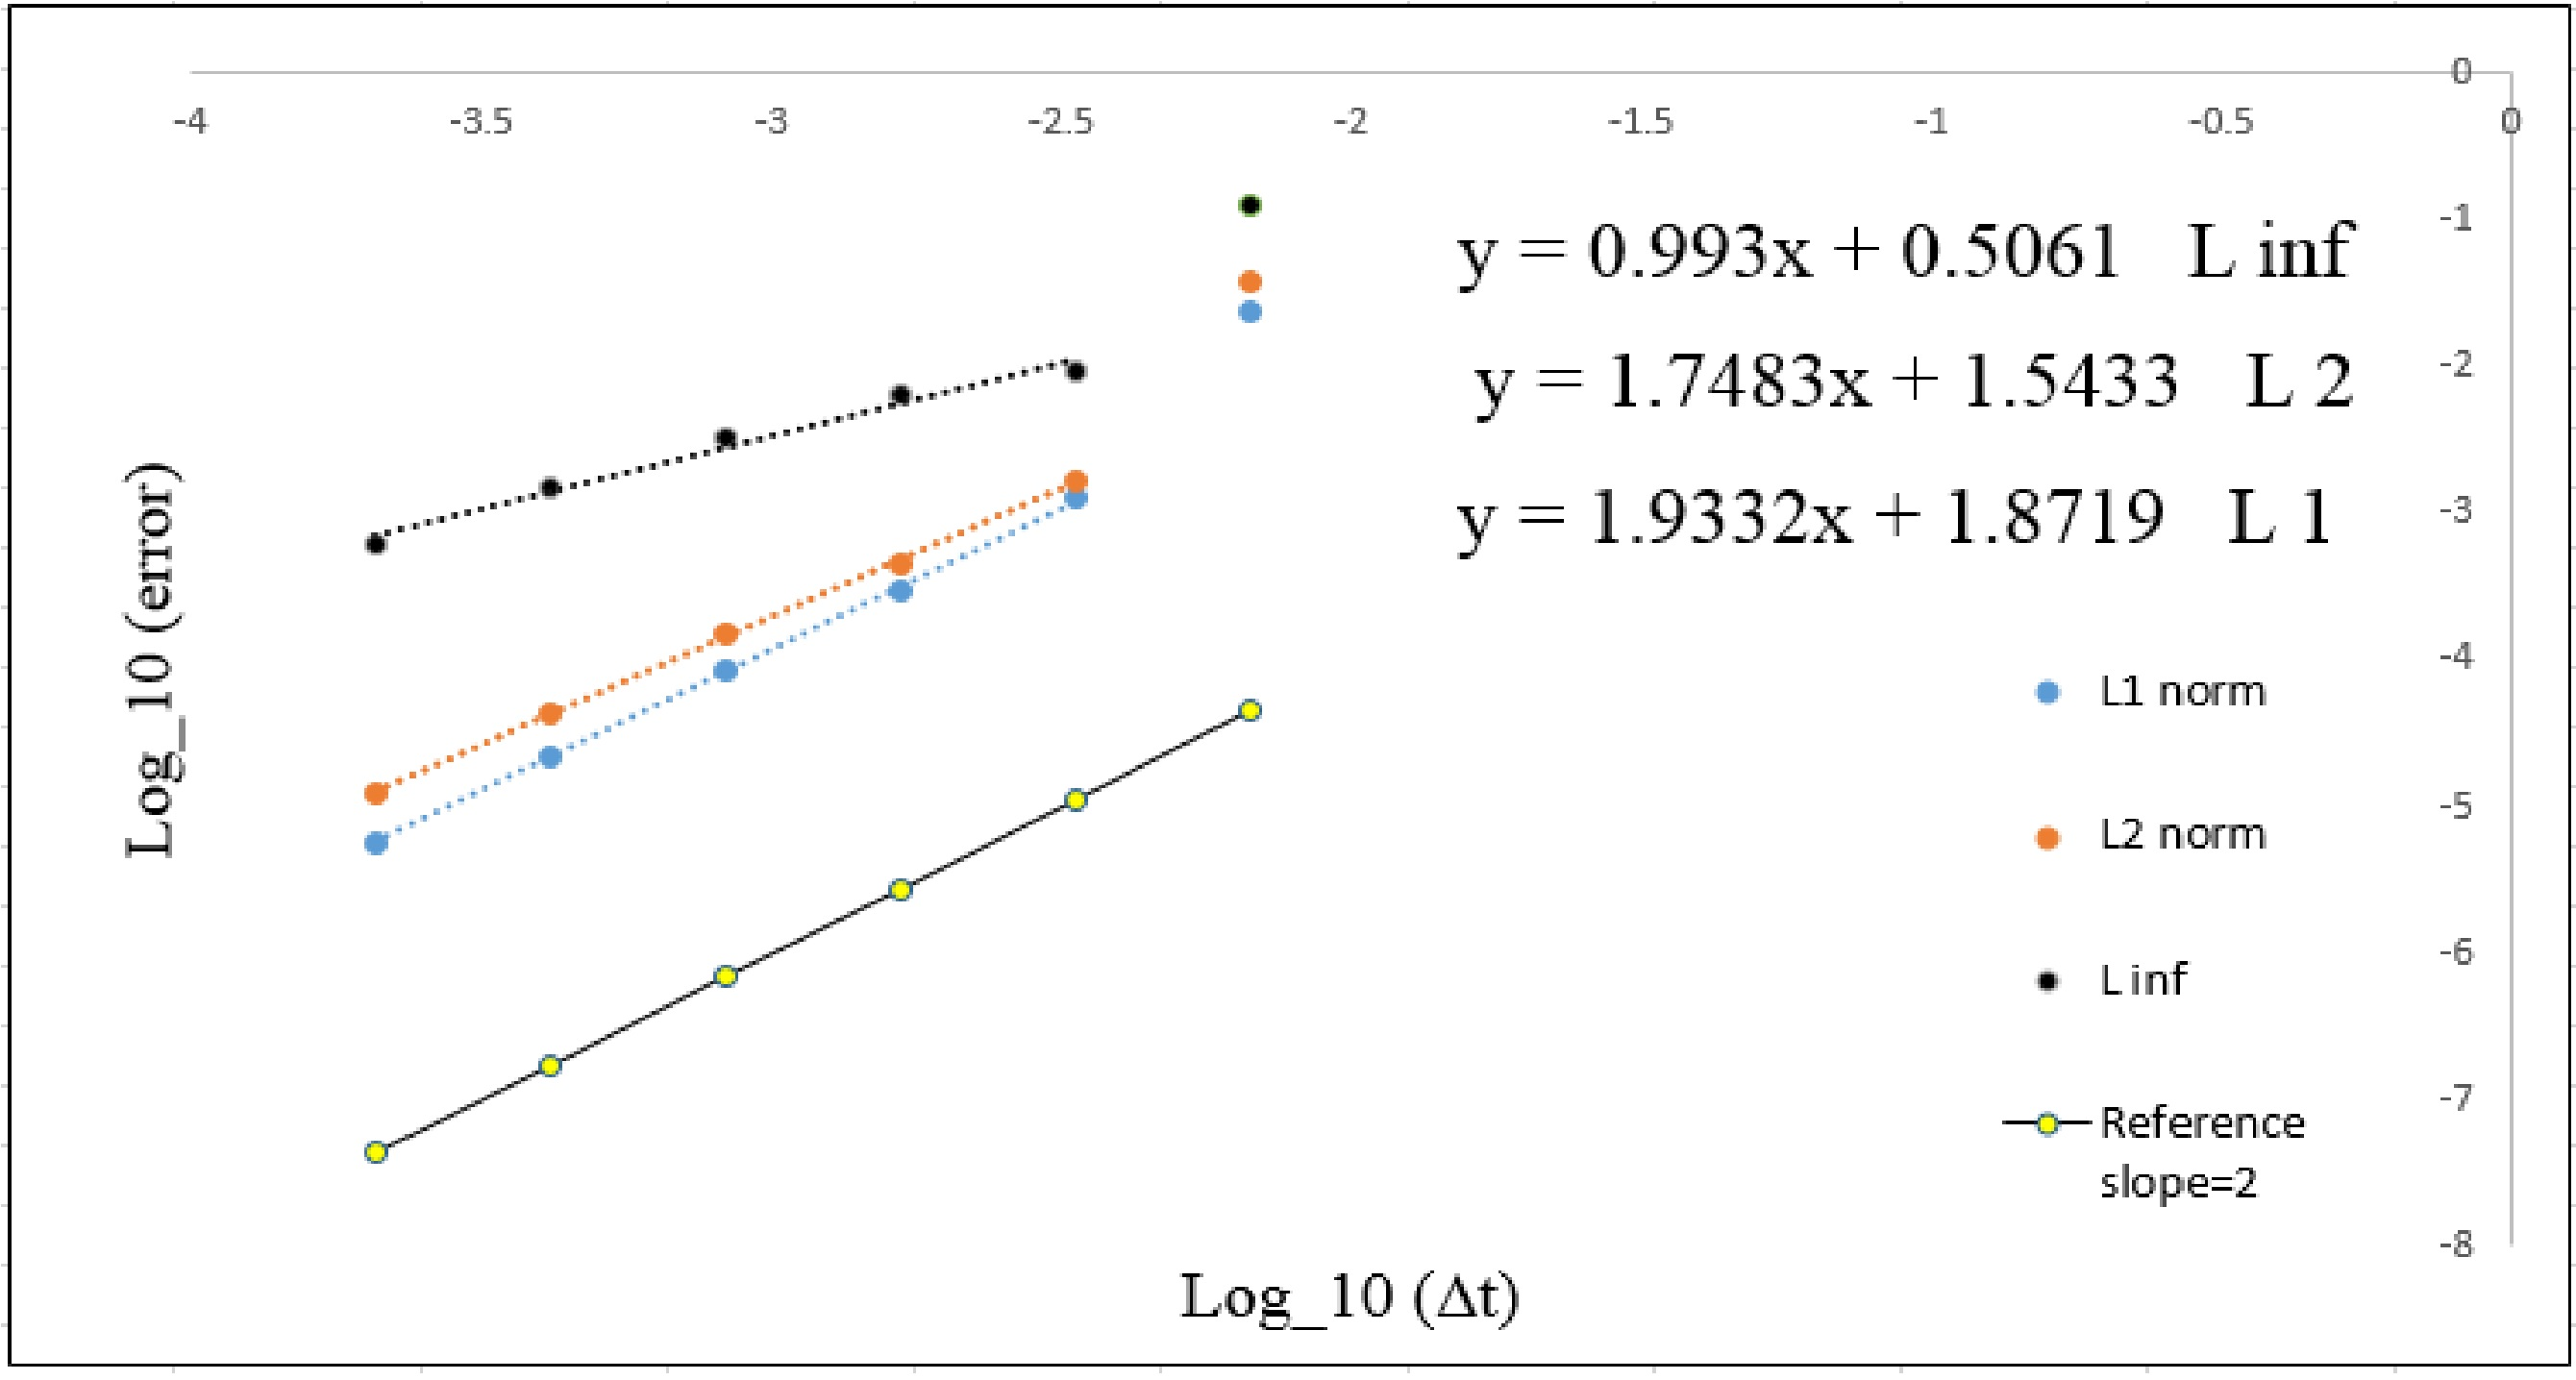
\includegraphics[width=4.5in]{figures/Pm1b_pf2_np_P_rate_c_0_5.jpg}}
		\caption{Log-Log plot of Convergence rate for Pressure}\label{fig:6.19a}		
	\end{subfigure}
	\quad
	\begin{subfigure}[t]{4.5in}
		\centering
		\scalebox{1.2}{
		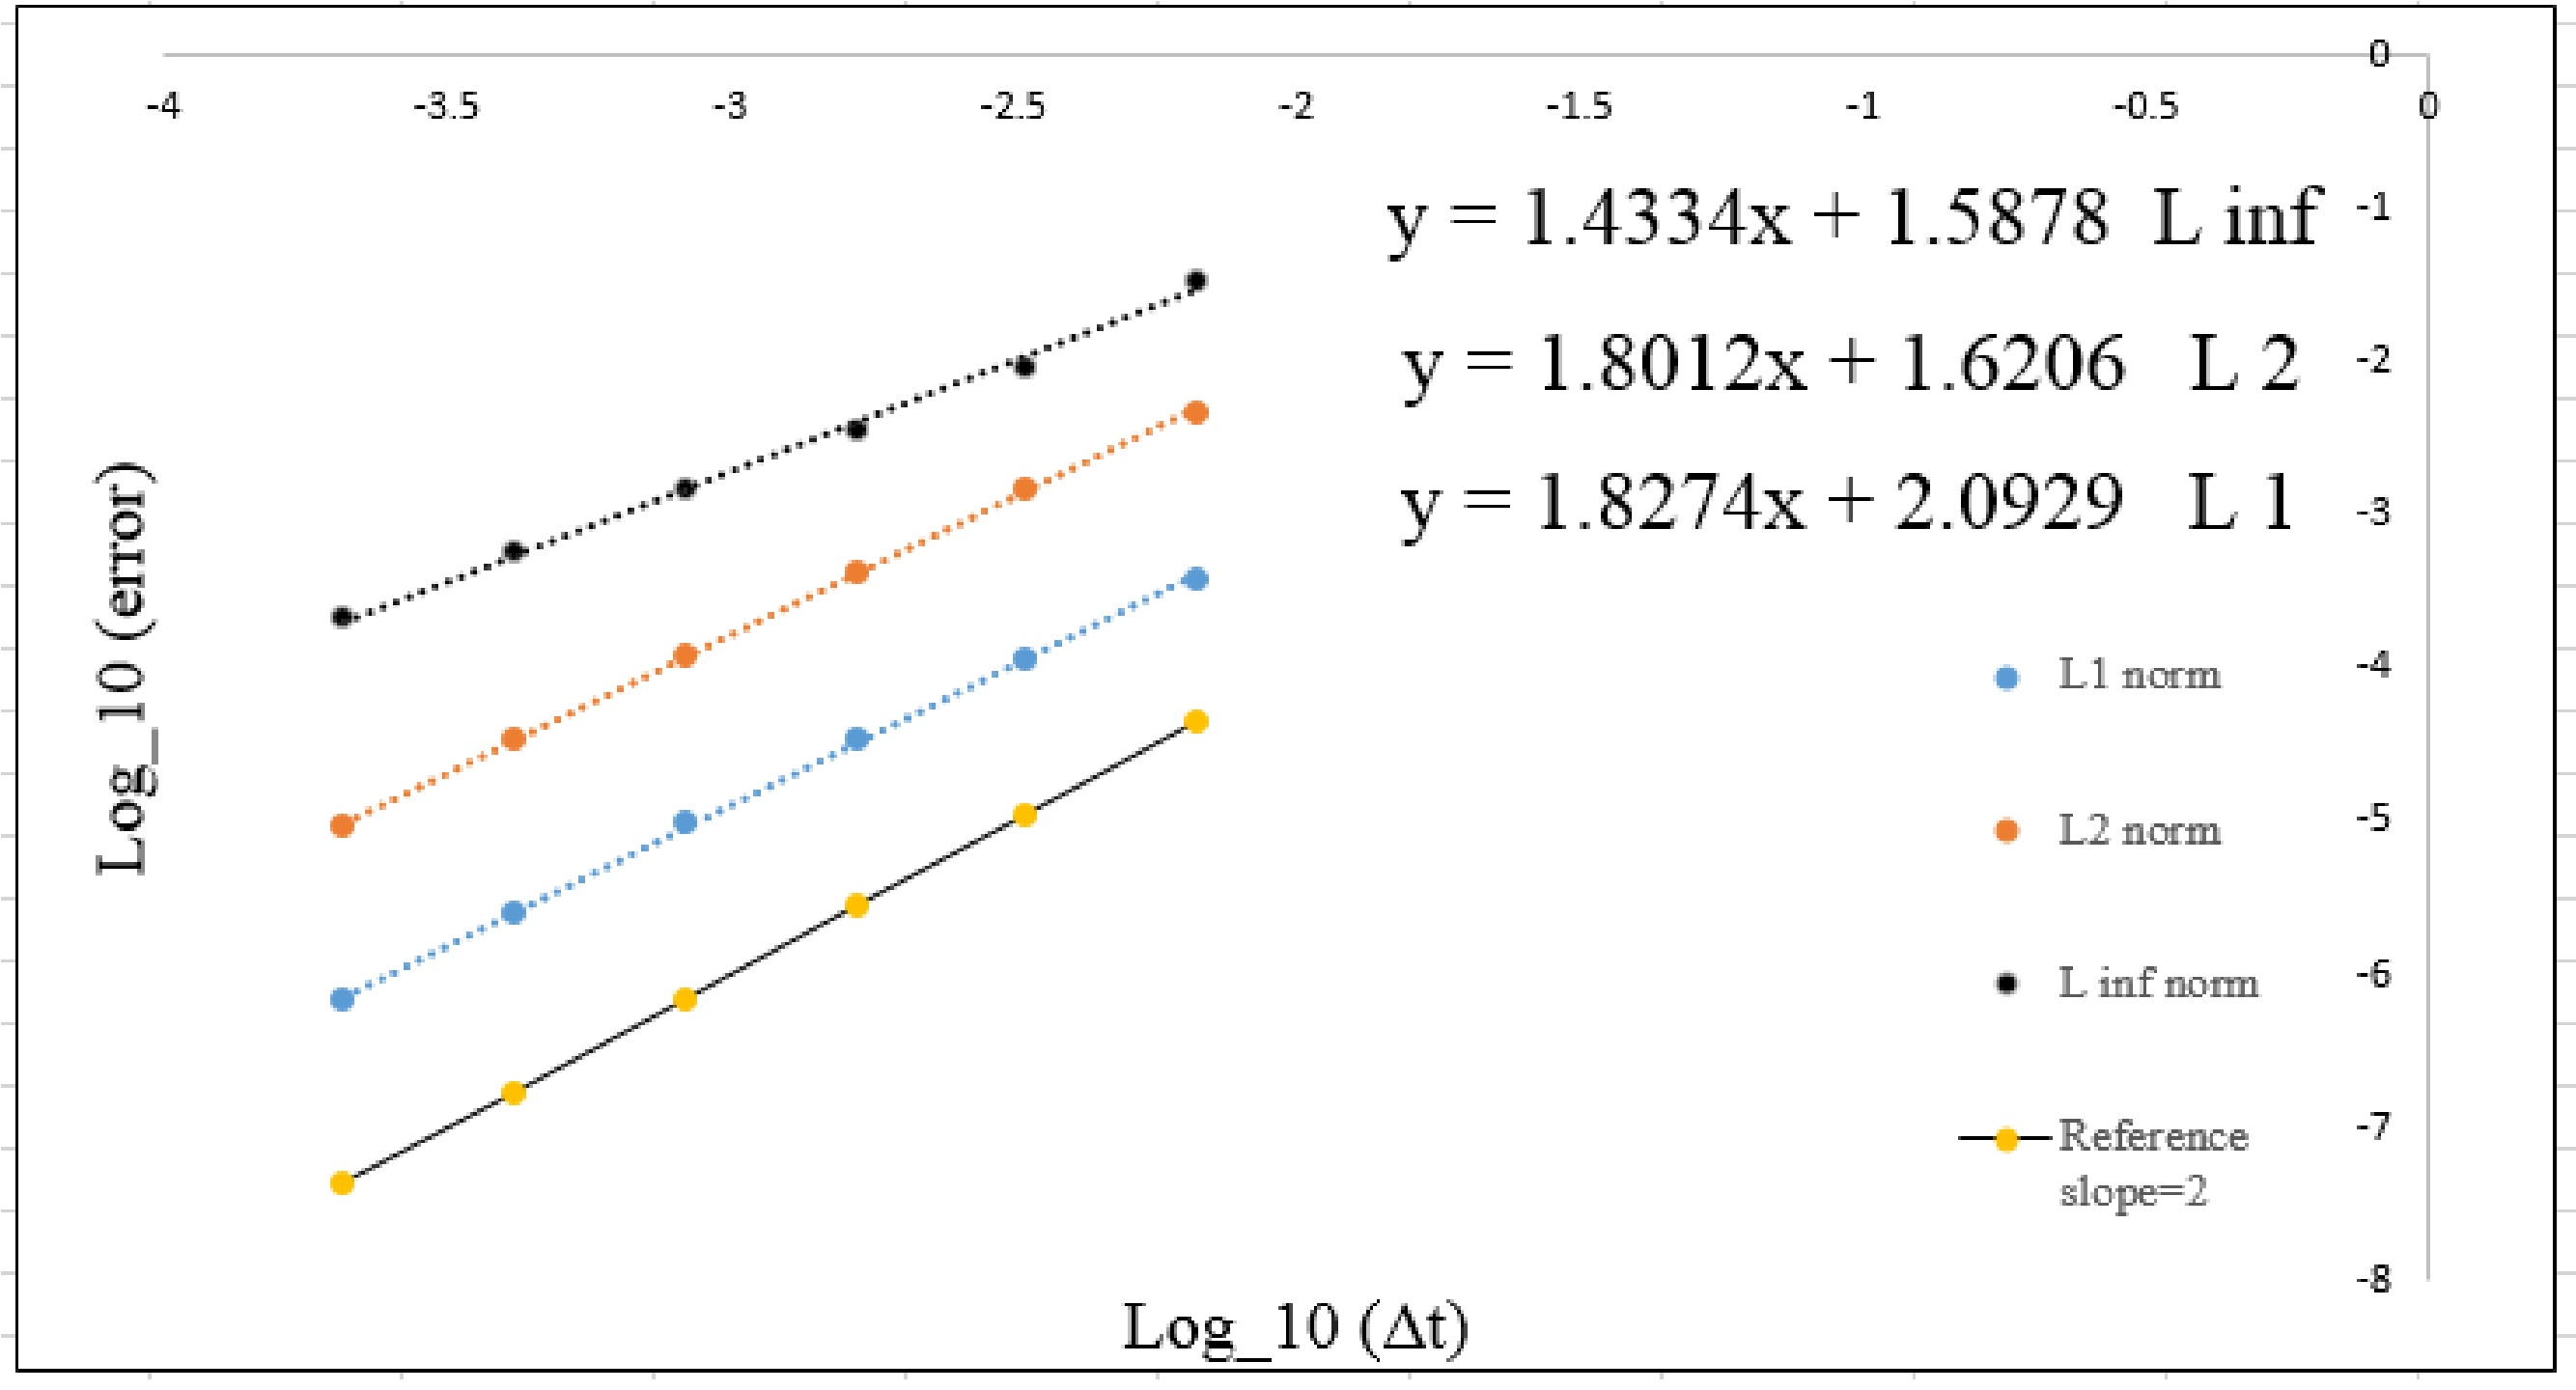
\includegraphics[width=4.5in]{figures/Pm1b_pf2_np_div_uv_rate_c_0_5.jpg}}
		\caption{Log-Log plot of Convergence rate for $\nabla \cdot \textbf{u}^*$. }\label{fig:6.19b}
	\end{subfigure}
	\caption{Plot of Convergence rates for Alg 2 with Normalised Pressure approach used. Domain: $[-1,1]^2$, time = 1 and CFL = 0.5. In each plot, the data points corresponding to grid sizes of 15, 30, 60, 120, 240, and 480. Subplot (b) shows the error in the divergence of intermediate velocity. The data points between different norms are close to each. Hence $L_1$ and $L_\infty$ norms were shifted up and down by 0.5 respectively to distinguish from $L_2$ norm data points.}\label{fig:6.16}
\end{figure}

\begin{figure}[H]
	\centering
	\begin{subfigure}[t]{4.5in}
		\centering
		\scalebox{1.2}{
		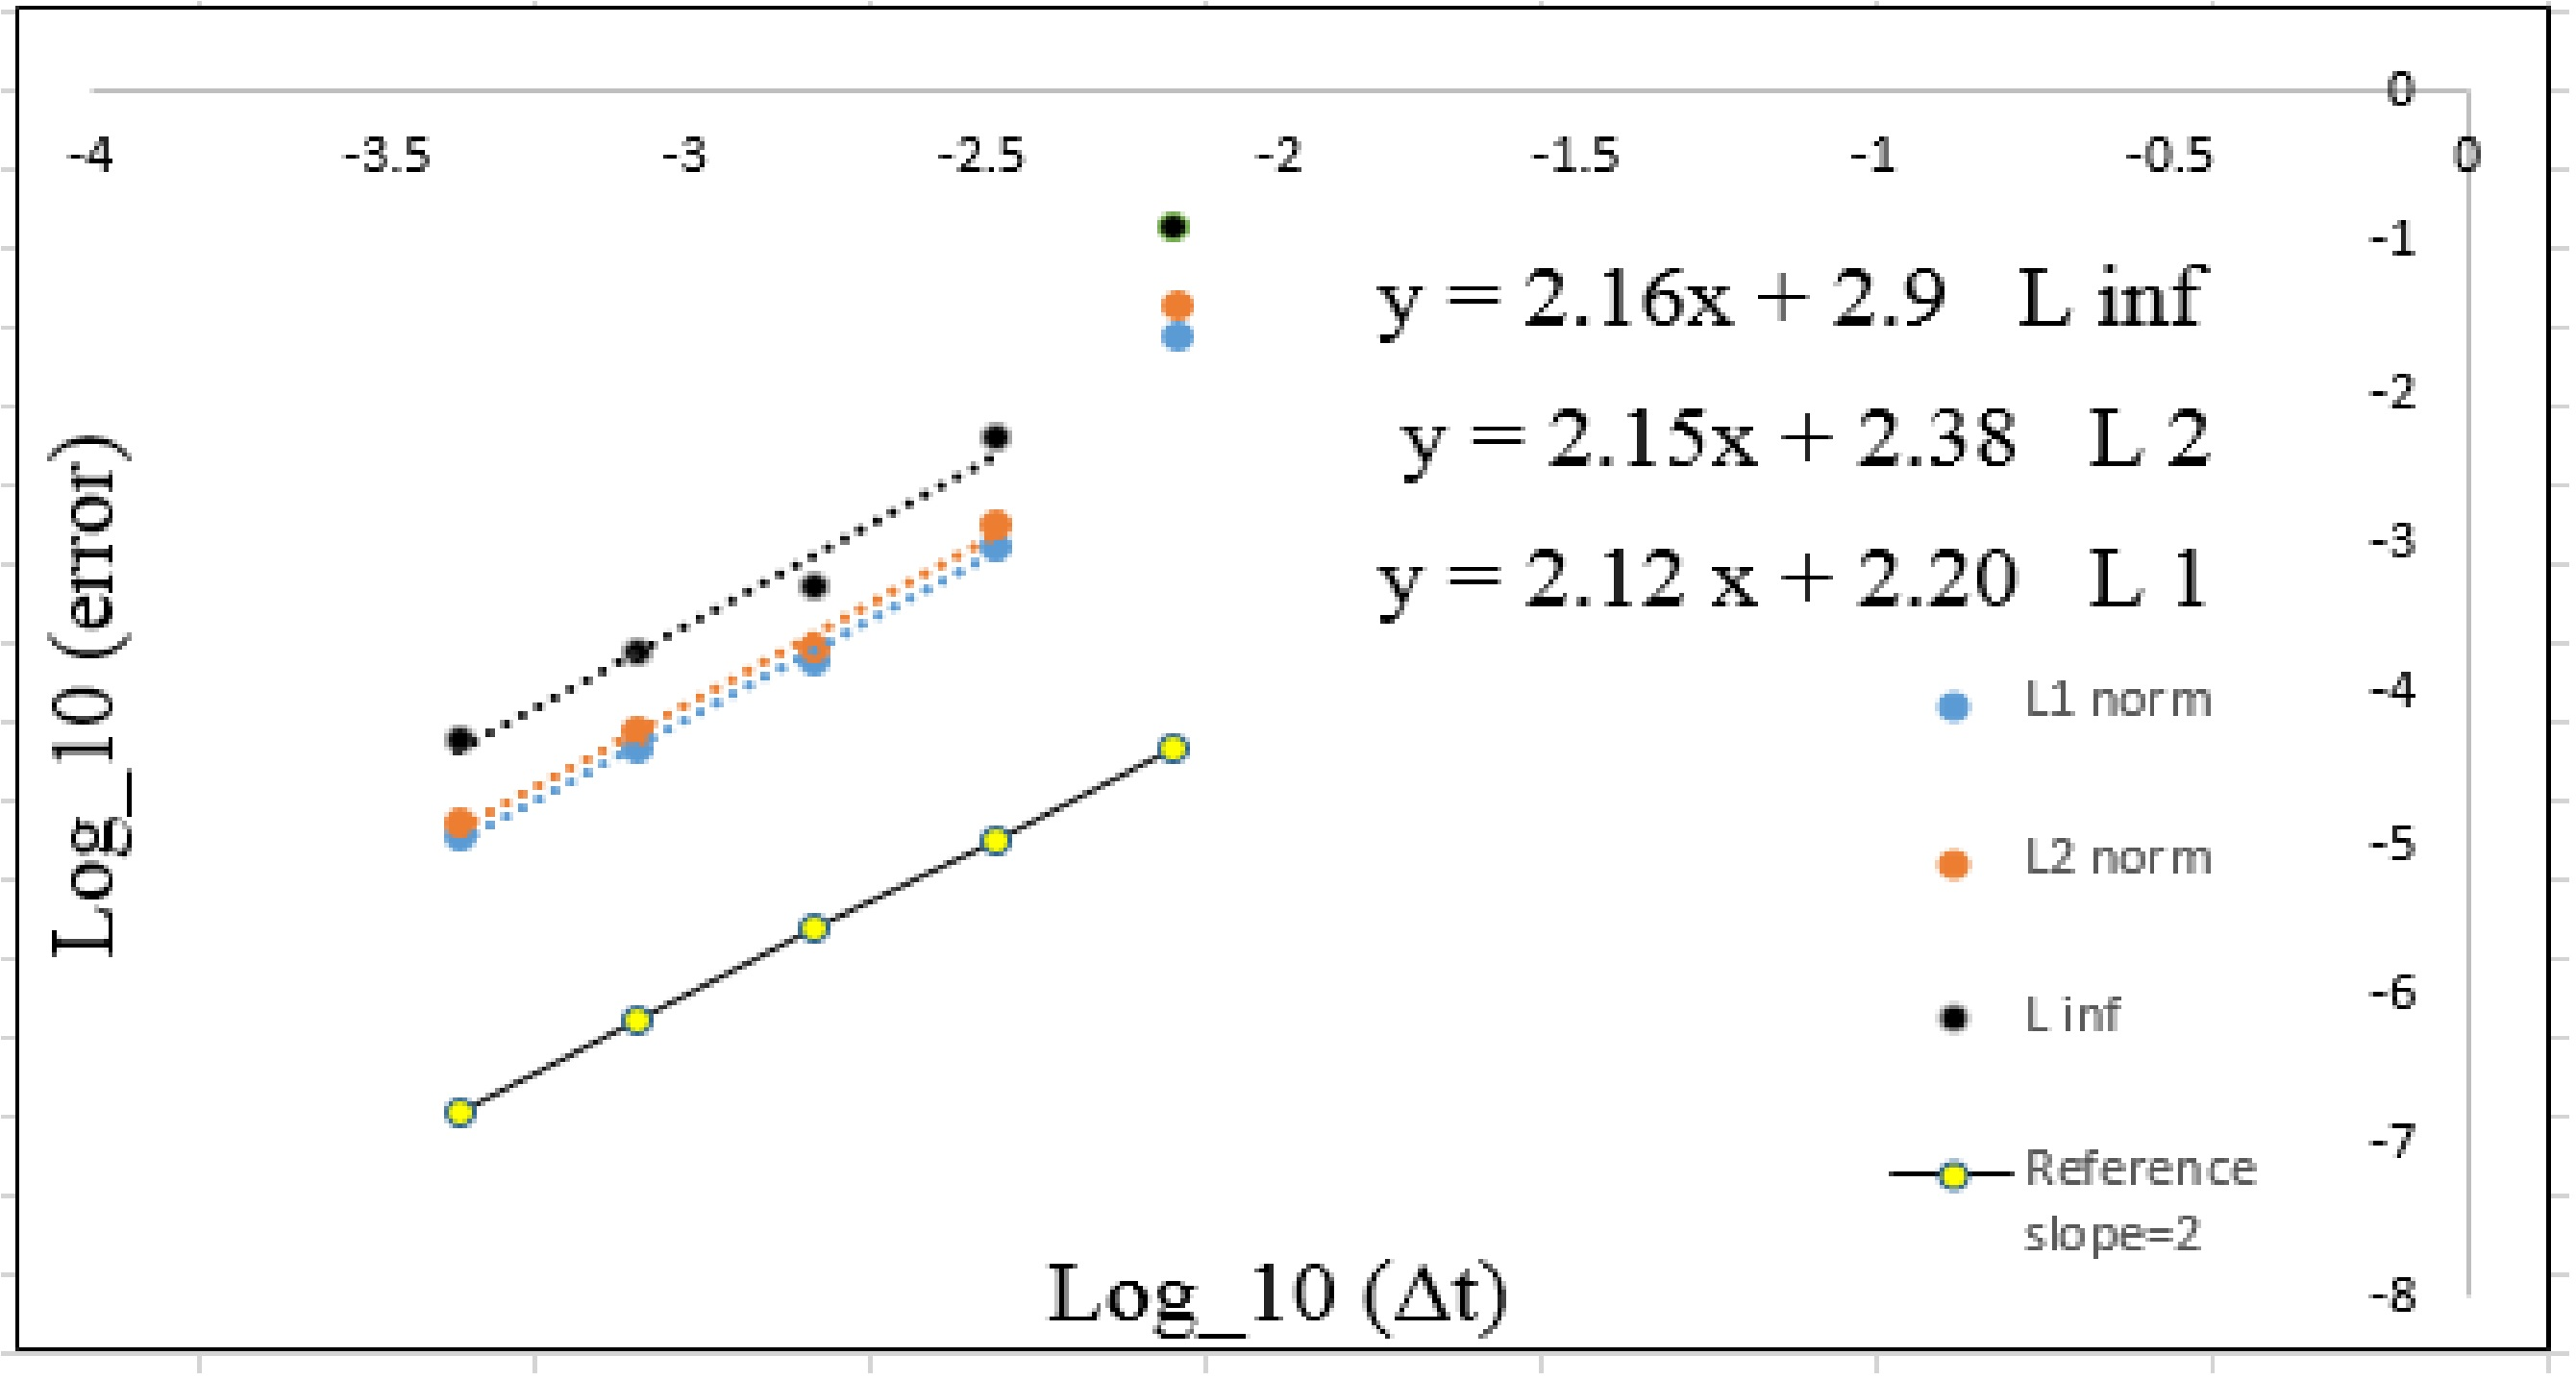
\includegraphics[width=4.5in]{figures/Pm2_pf2_np_P_rate_c_0_5.jpg}}
		\caption{Log-Log plot of Convergence rate for Pressure}\label{fig:6.19a}		
	\end{subfigure}
	\quad
	\begin{subfigure}[t]{4.5in}
		\centering
		\scalebox{1.2}{
		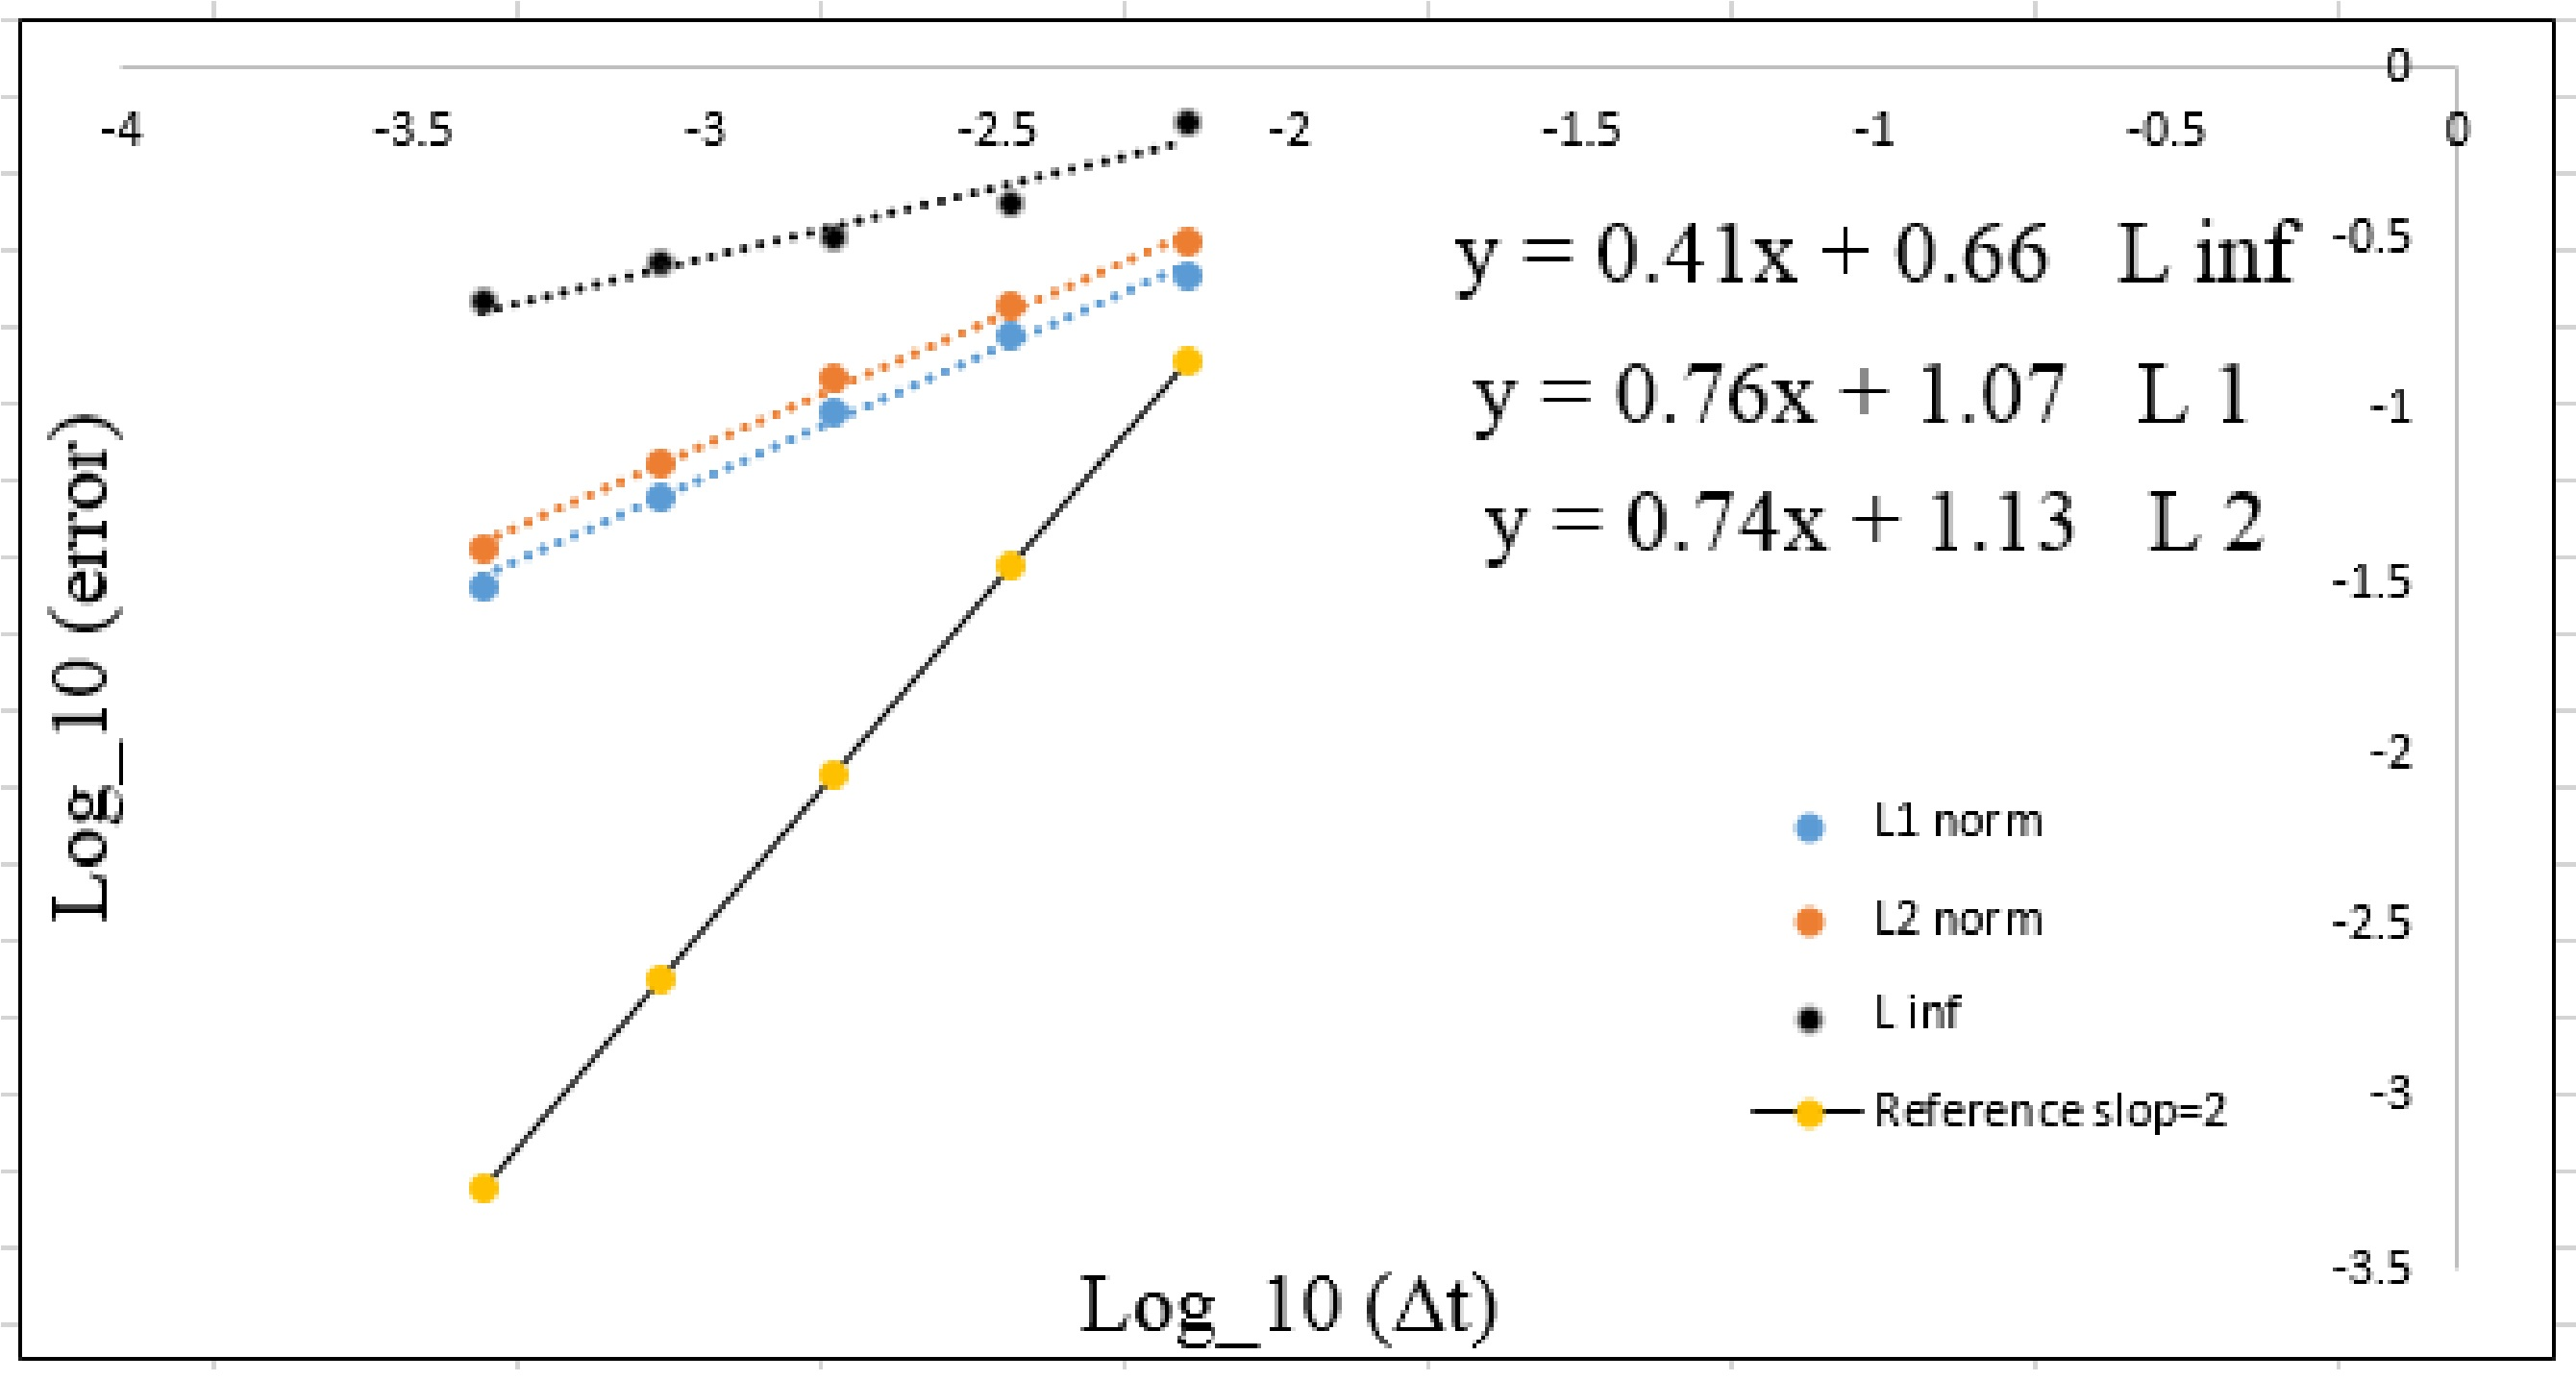
\includegraphics[width=4.5in]{figures/Pm2_pf2_np_div_uvstar_rate_c_0_5.jpg}}
		\caption{Log-Log plot of Convergence rate for $\nabla \cdot \textbf{u}^*$. }\label{fig:6.19b}
	\end{subfigure}
	\caption{Plot of Convergence rates for Alg 3 with Normalised Pressure approach used. Domain: $[-1,1]^2$, time = 1 and CFL = 0.5. In each plot, the data points corresponding to grid sizes of 15, 30, 60, 120, 240.}\label{fig:6.16}
\end{figure}

\begin{figure}[H]
	\centering
	\scalebox{1.2}{
	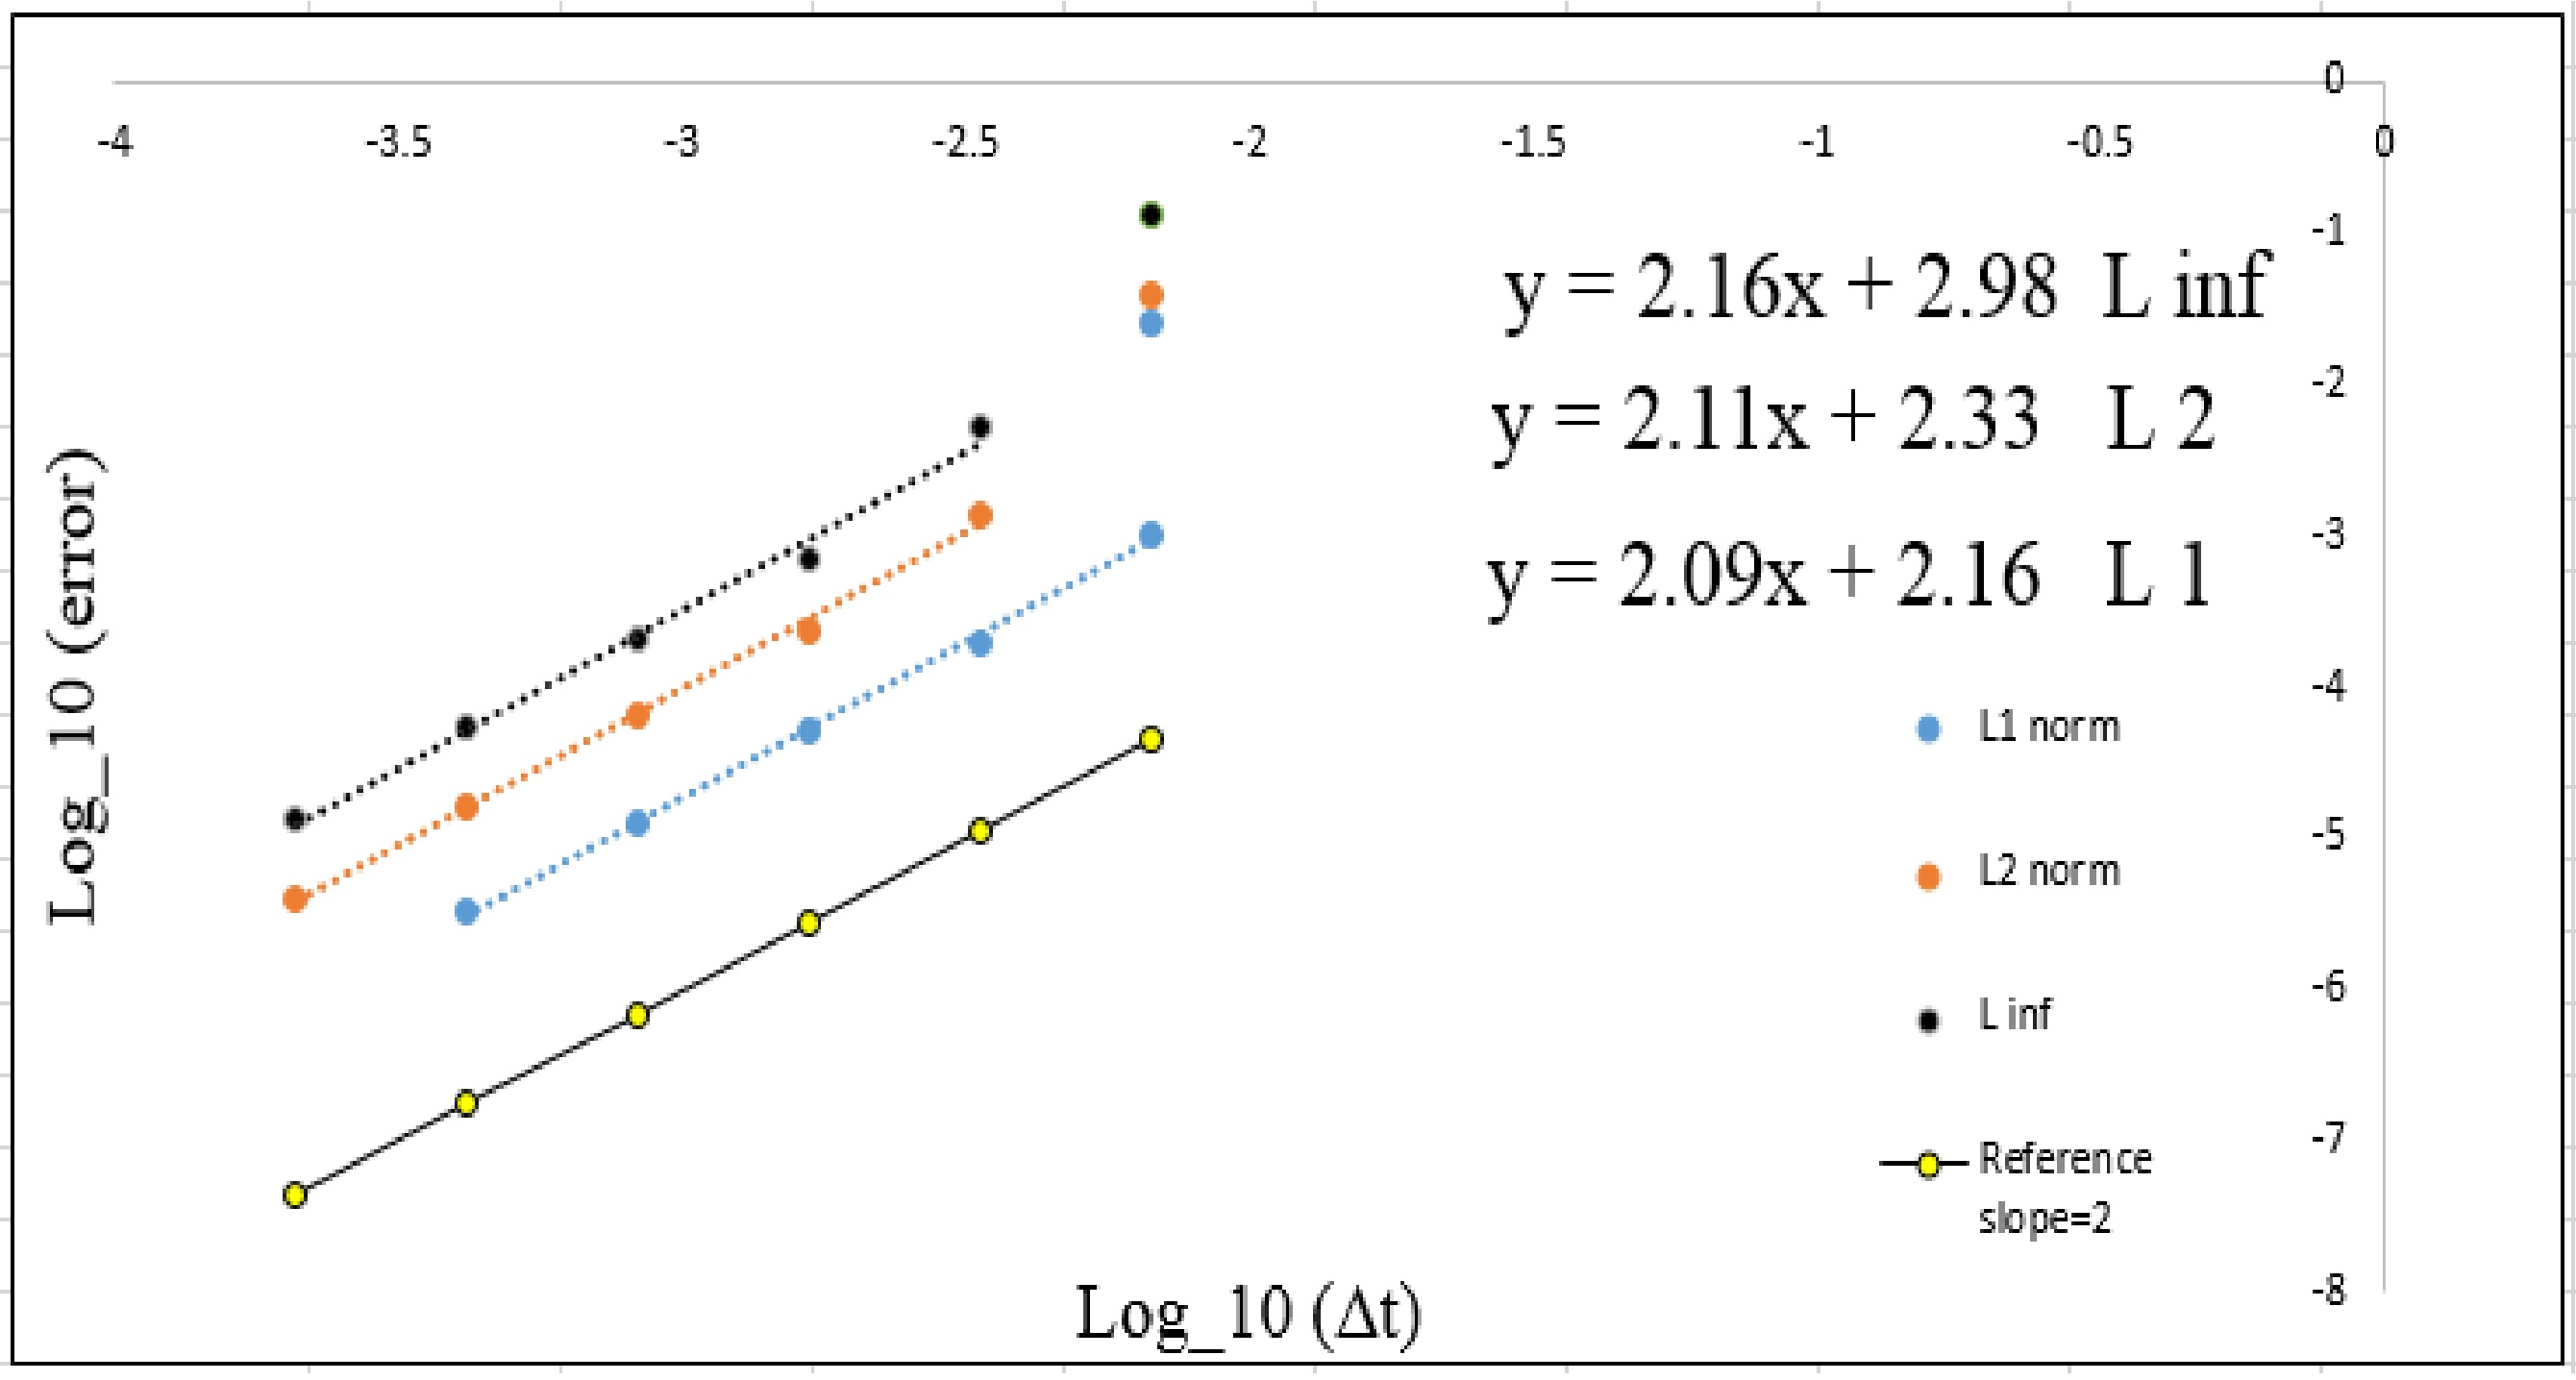
\includegraphics[width=4.5in]{figures/Gauge_pf2_np_P_rate_c_0_5.jpg}}
	\caption{Long-Log plot of Pressure Convergence rates for Gauge method with Normalised Pressure approach used. Domain: $[-1,1]^2$, time = 1 and CFL = 0.5. The data points corresponding to grid sizes of 15, 30, 60, 120, 240, and 480.}\label{fig:6.16}
\end{figure}

\begin{figure}[H]
	\centering
	\begin{subfigure}[t]{2.2in}
		\centering
		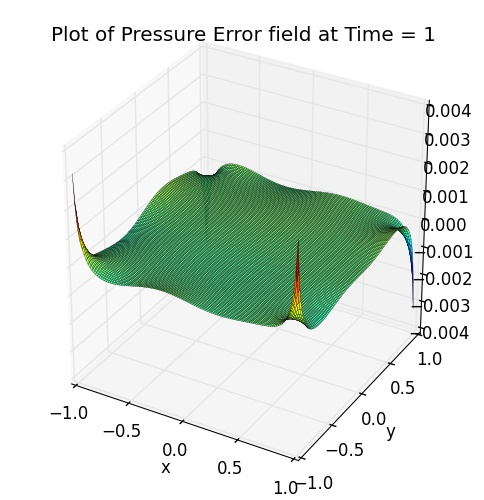
\includegraphics[width=2.2in]{figures/Pm1b_pf2_np_P_error_t_1_grid_120.jpg}
		\caption{Pressure error field for Alg 2 method}\label{fig:6.19a}		
	\end{subfigure}
	\quad
	\begin{subfigure}[t]{2.8in}
		\centering
		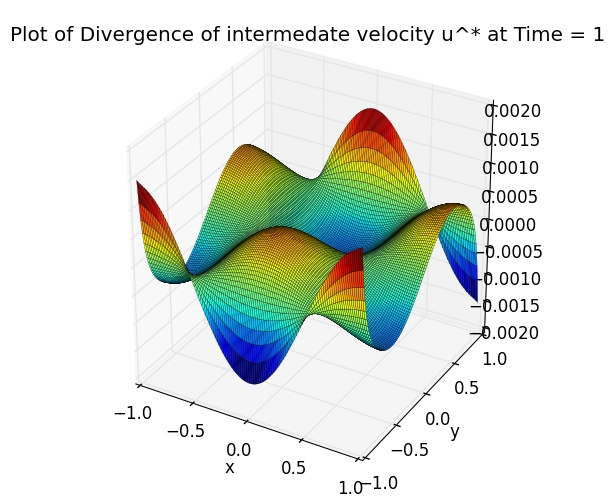
\includegraphics[width=2.8in]{figures/Pm1b_pf2_np_div_uvstar_t_1_grid_120.jpg}
		\caption{Divergence of intermediate velocity field for Alg 2 method. }\label{fig:6.19b}
	\end{subfigure}
	\quad
	\centering
	\begin{subfigure}[t]{2.2in}
		\centering
		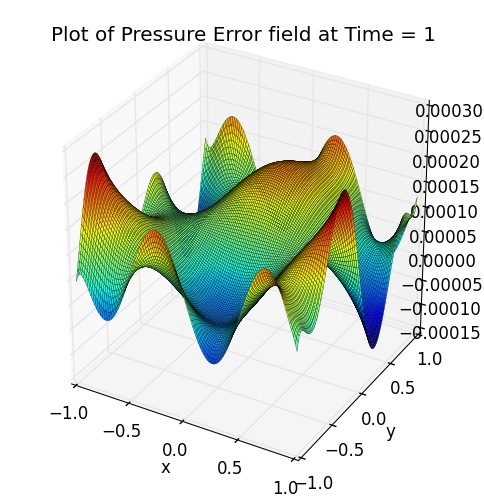
\includegraphics[width=2.2in]{figures/Pm2_pf2_cN_np_P_error_t_1_grid_120.jpg}
		\caption{Pressure error field for Alg 3 method}\label{fig:6.19c}		
	\end{subfigure}
	\quad
	\begin{subfigure}[t]{2.6in}
		\centering
		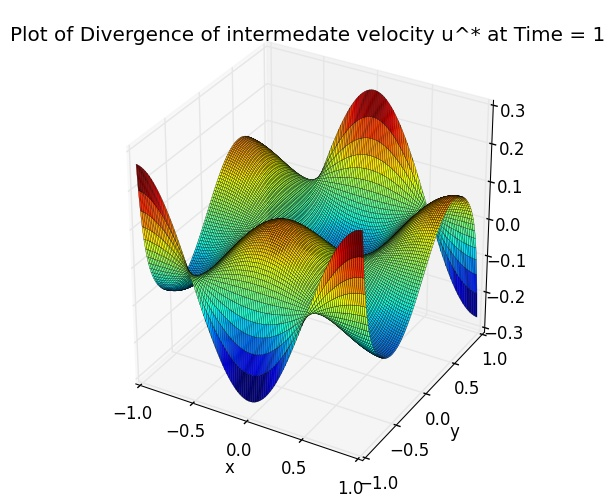
\includegraphics[width=2.6in]{figures/Pm2_pf2_cN_np_div_uvstar_t_1_grid_120.jpg}
		\caption{Divergence of intermediate velocity field for Alg 3 method.}\label{fig:6.19d}
	\end{subfigure}
	\quad
	\begin{subfigure}[t]{2.5in}
		\centering
		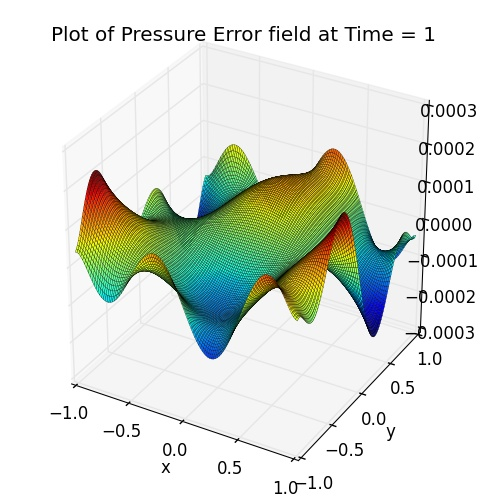
\includegraphics[width=2.5in]{figures/Gauge_pf2_P_error_t_1_grid_120.jpg}
		\caption{Pressure error field for Gauge method. }\label{fig:6.19d}
	\end{subfigure}
	\caption{Plots of Pressure error fields and divergence of intermediate velocity for Alg 2, Alg 3 and Gauge method at grid size of 120. Domain: $[-1,1]^2$, time = 1 and CFL = 0.5. }\label{fig:6.16}
\end{figure}

\subsection*{Periodic boundary}
To investigate the performance of projection methods in different boundary conditions, we have implemented a periodic boundary condition in y in order to mimic a periodic channel geometry. The same forced flow problem is considered, but in domain $[-\dfrac{1}{2},\dfrac{1}{2}]^2$. Periodic boundary is ensured by putting the ``ghost cell" values at one side of domain to be equal to the interior points just next to the opposite boundary. For instance, for $U$ velocity at the South boundary ($y = -\dfrac{1}{2}$) we impose the condition: $u_{i-1/2,0} = u_{i-1/2,m}$. This eliminates the spatial interpolation error occurred in calculating the ``ghost cell" values. The exact solutions are once again illustrated below in Figure 6.7. The convergence rates in pressure are also summarised.\\

Interestingly, this time we see all the methods including Alg 2 show second order error convergence in pressure! The $L_\infty$ in Alg 2 is improved to 1.90 (as compared to 1.01 in the previous domain). The pressure error fields and the plot of divergence of intermediate velocity fields for projection methods are also more smooth now. In fact the pressure error fields for Alg 2, Alg 3 and the Gauge method is very similar now, indicating that the periodic geometry recovers second order accuracy for projection methods. This is in agreement with our normal mode analysis done before in Chapter 4 and this also indicate the projection methods (in particular Alg 2) only show optimal pressure error convergence in special domains like the periodic boundary domain whereas the Gauge method shows optimal convergence in general domains too. This finding is in support of Shen et.al results \cite{guermond2004error, guermond2006overview} where they have also given an error bound of 1.5 for projection method (Alg 2 in particular). This shows a limitation in normal mode analysis too. The exact cause of this problem however still remains open in literature.\\

\begin{figure}[H]
	\centering
	\begin{subfigure}[t]{2.5in}
		\centering
		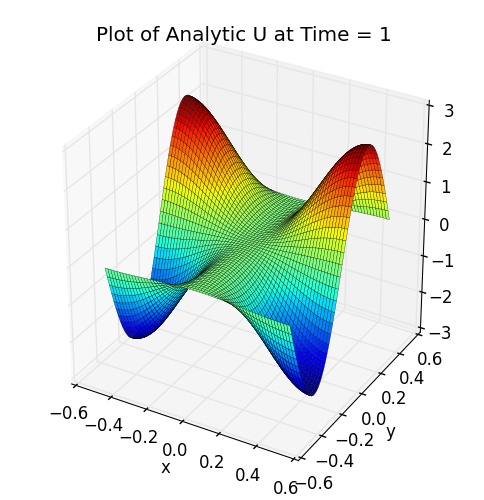
\includegraphics[width=2.5in]{figures/Pm1b_pf2b_U_exact_t_1_grid_60.jpg}
		\caption{Analytic $U$ velocity at $t=1$}\label{fig:7.1a}		
	\end{subfigure}
	\quad
	\begin{subfigure}[t]{2.5in}
		\centering
		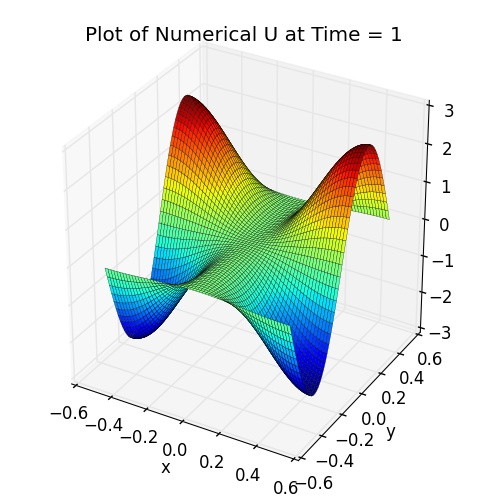
\includegraphics[width=2.5in]{figures/Pm1b_pf2b_uf_t_1_grid_60.jpg}
		\caption{Numerical $U$ velocity at $t=1$}\label{fig:7.1b}
	\end{subfigure}
	\quad
	\begin{subfigure}[t]{2.5in}
		\centering
		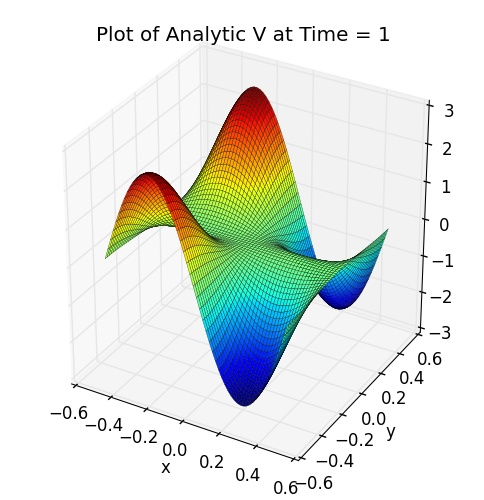
\includegraphics[width=2.5in]{figures/Pm1b_pf2b_V_exact_t_1_grid_60.jpg}
		\caption{Analytic $V$ velocity at $t=1$}\label{fig:7.1c}
	\end{subfigure}
	\quad
	\begin{subfigure}[t]{2.5in}
		\centering
		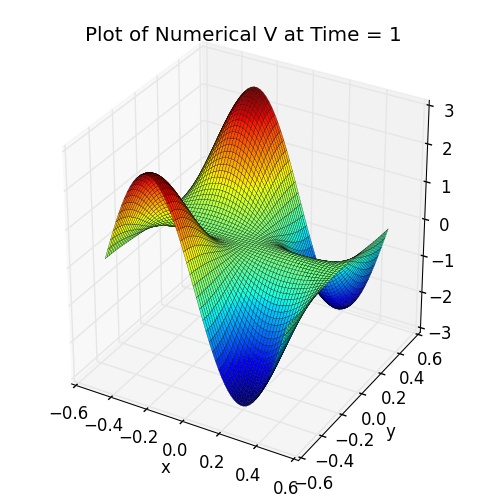
\includegraphics[width=2.5in]{figures/Pm1b_pf2b_vf_t_1_grid_60.jpg}
		\caption{Numerical $V$ velocity at $t=1$}\label{fig:7.1d}
	\end{subfigure}
	\quad	
	\begin{subfigure}[t]{2.5in}
		\centering
		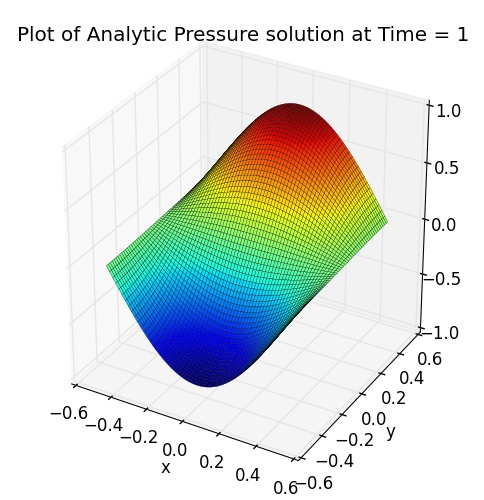
\includegraphics[width=2.5in]{figures/Pm1b_pf2b_P_exact_t_1_grid_60.jpg}
		\caption{Analytic pressure ($P$) at $t=1$}\label{fig:7.1e}
	\end{subfigure}
	\quad	
	\begin{subfigure}[t]{2.5in}
		\centering
		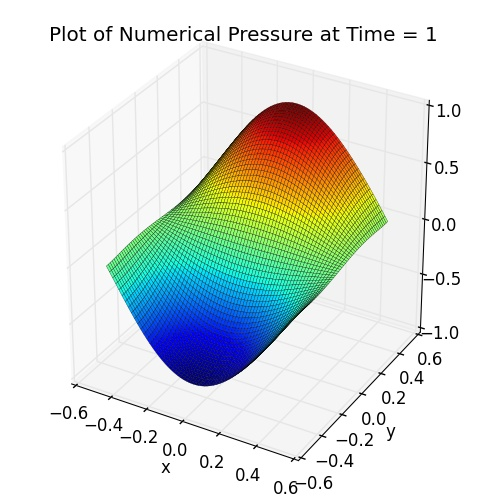
\includegraphics[width=2.5in]{figures/Pm1b_pf2b_pf_t_1_grid_60.jpg}
		\caption{Numerical pressure ($P$) at $t=1$}\label{fig:7.1f}
	\end{subfigure}
	\caption{Plot of exact and numerical solutions ($U,V,P$) at time $t=1$ on the spatial domain of $[-\dfrac{1}{2},\dfrac{1}{2}]^2$ with grid size $60 \times 60$. Alg 2 method is used to compute the numerical solutions with $CFL=0.5$}\label{fig:7.1}
\end{figure}

\begin{figure}[H]
	\centering
	\begin{subfigure}[t]{4.5in}
		\centering
		\scalebox{1.2}{
		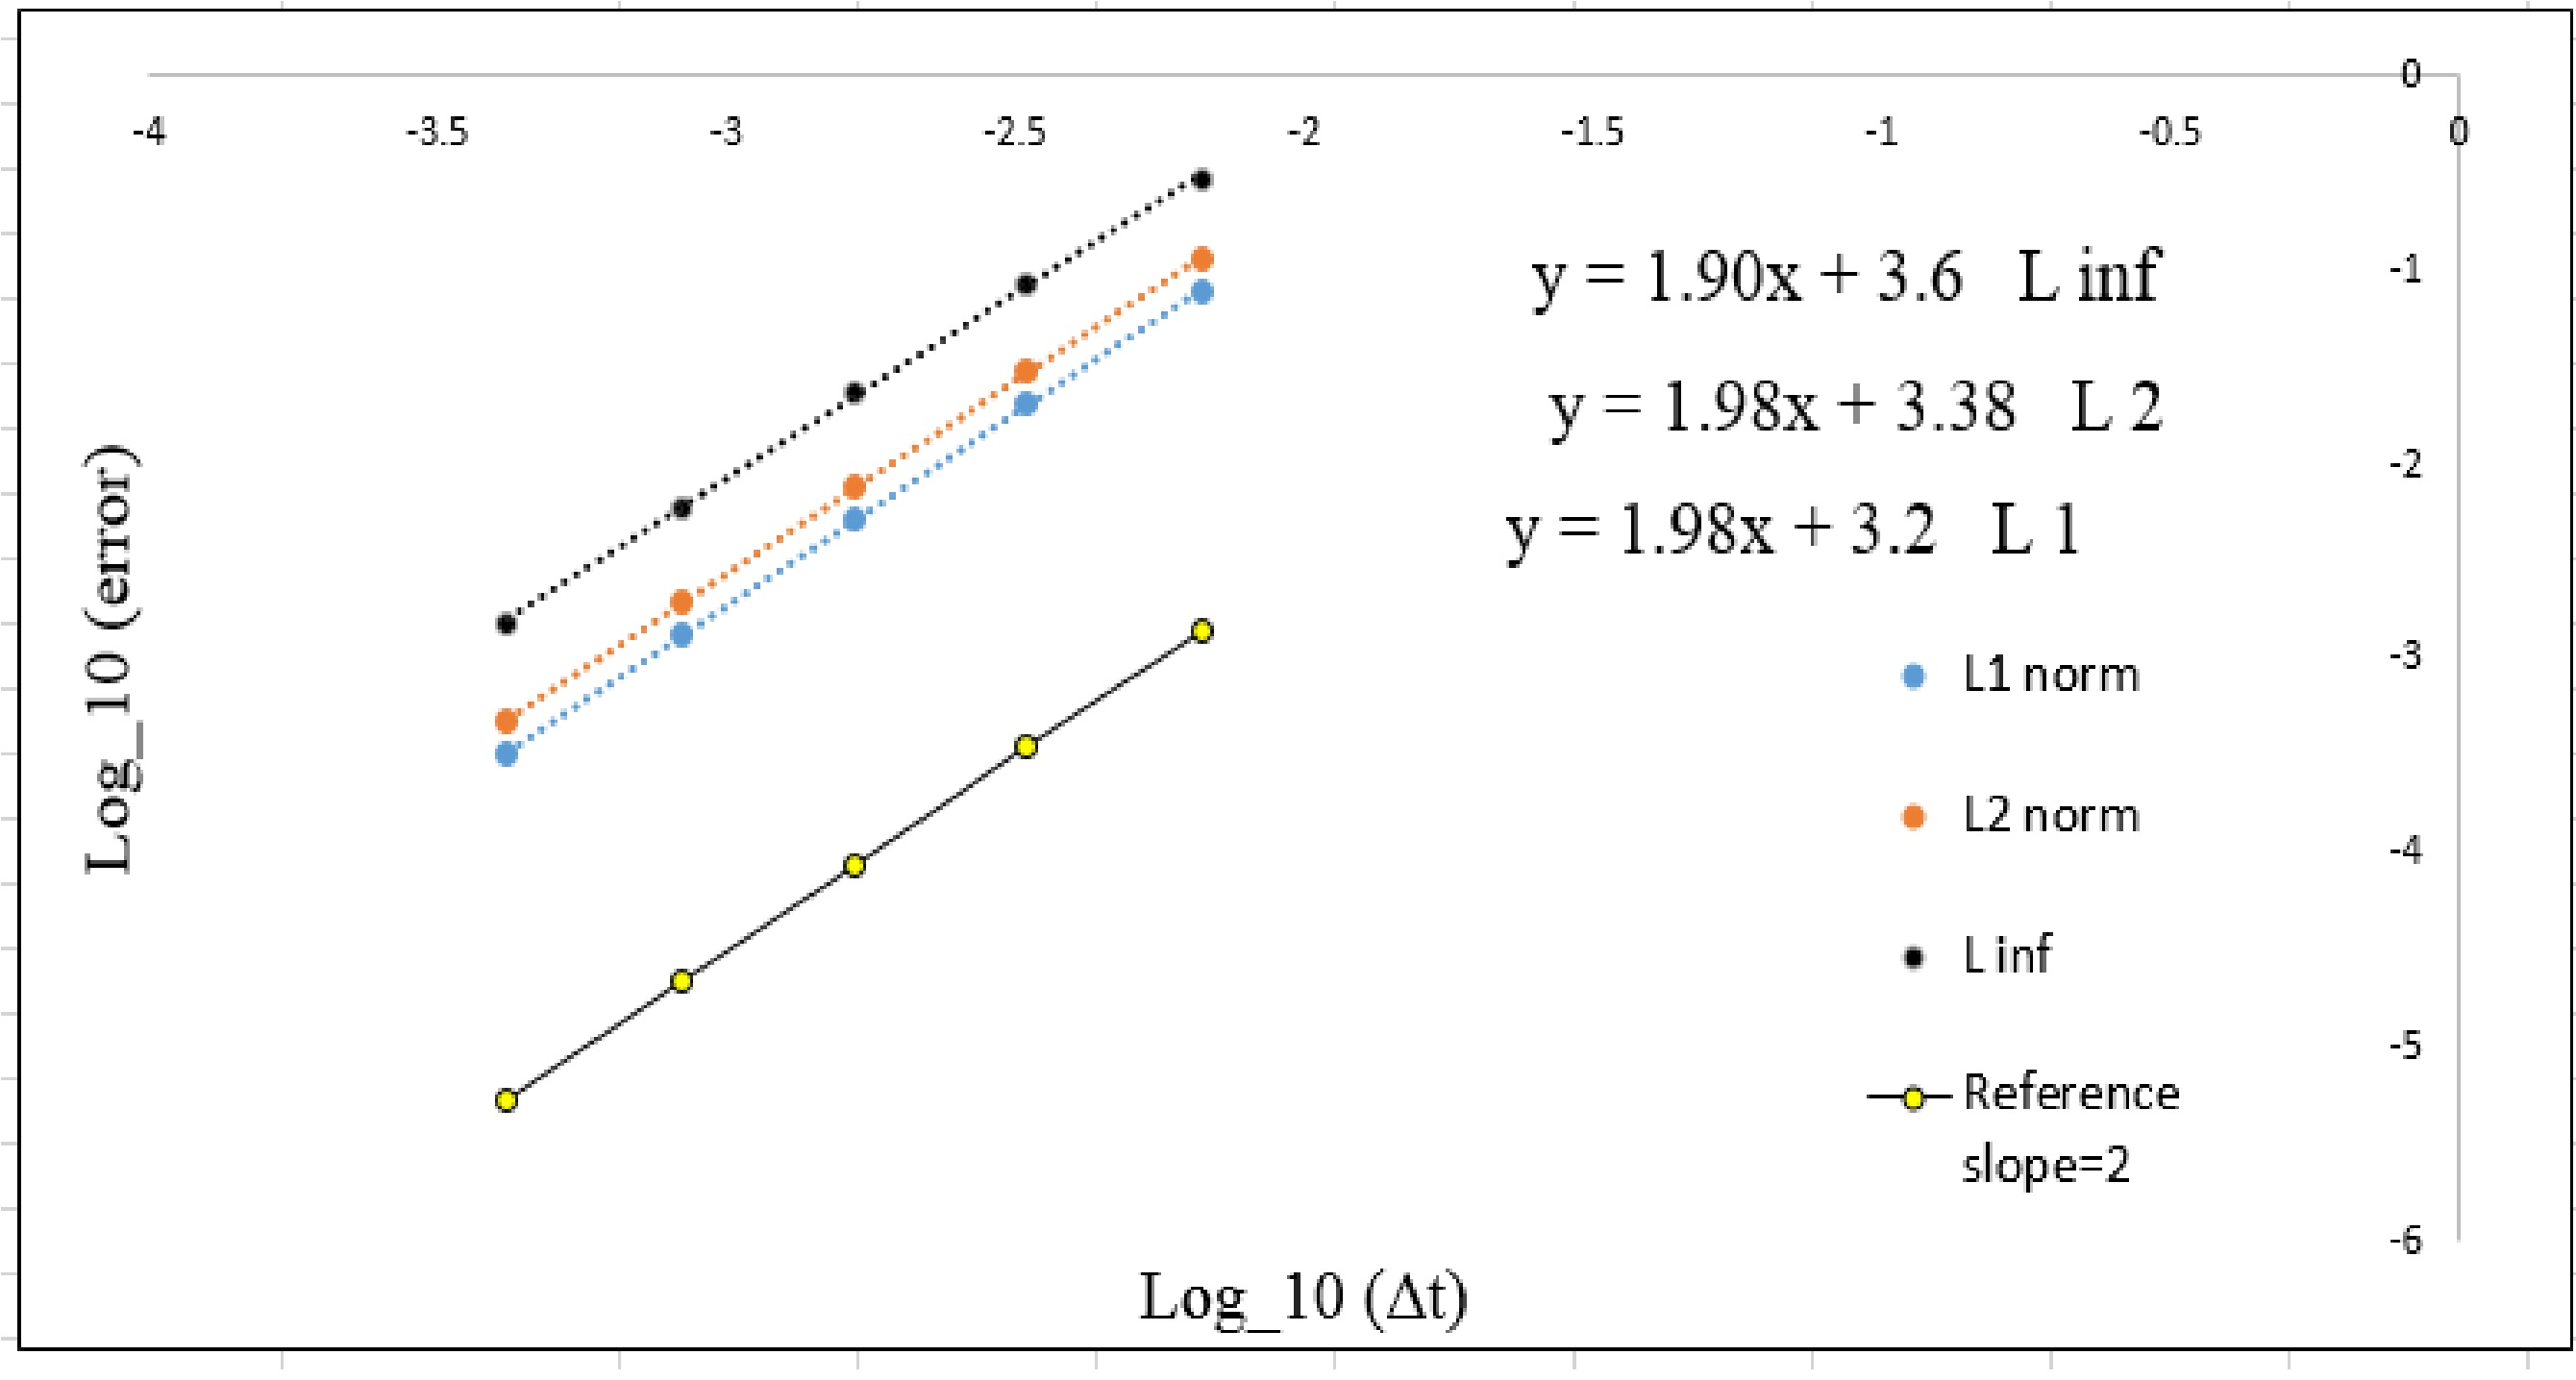
\includegraphics[width=4.5in]{figures/Pm1b_pf2b_np_P_rate_c_0_5.jpg}}
		\caption{Log-Log plot of Convergence rate for Pressure}\label{fig:6.19a}		
	\end{subfigure}
	\quad
	\begin{subfigure}[t]{4.5in}
		\centering
		\scalebox{1.2}{
		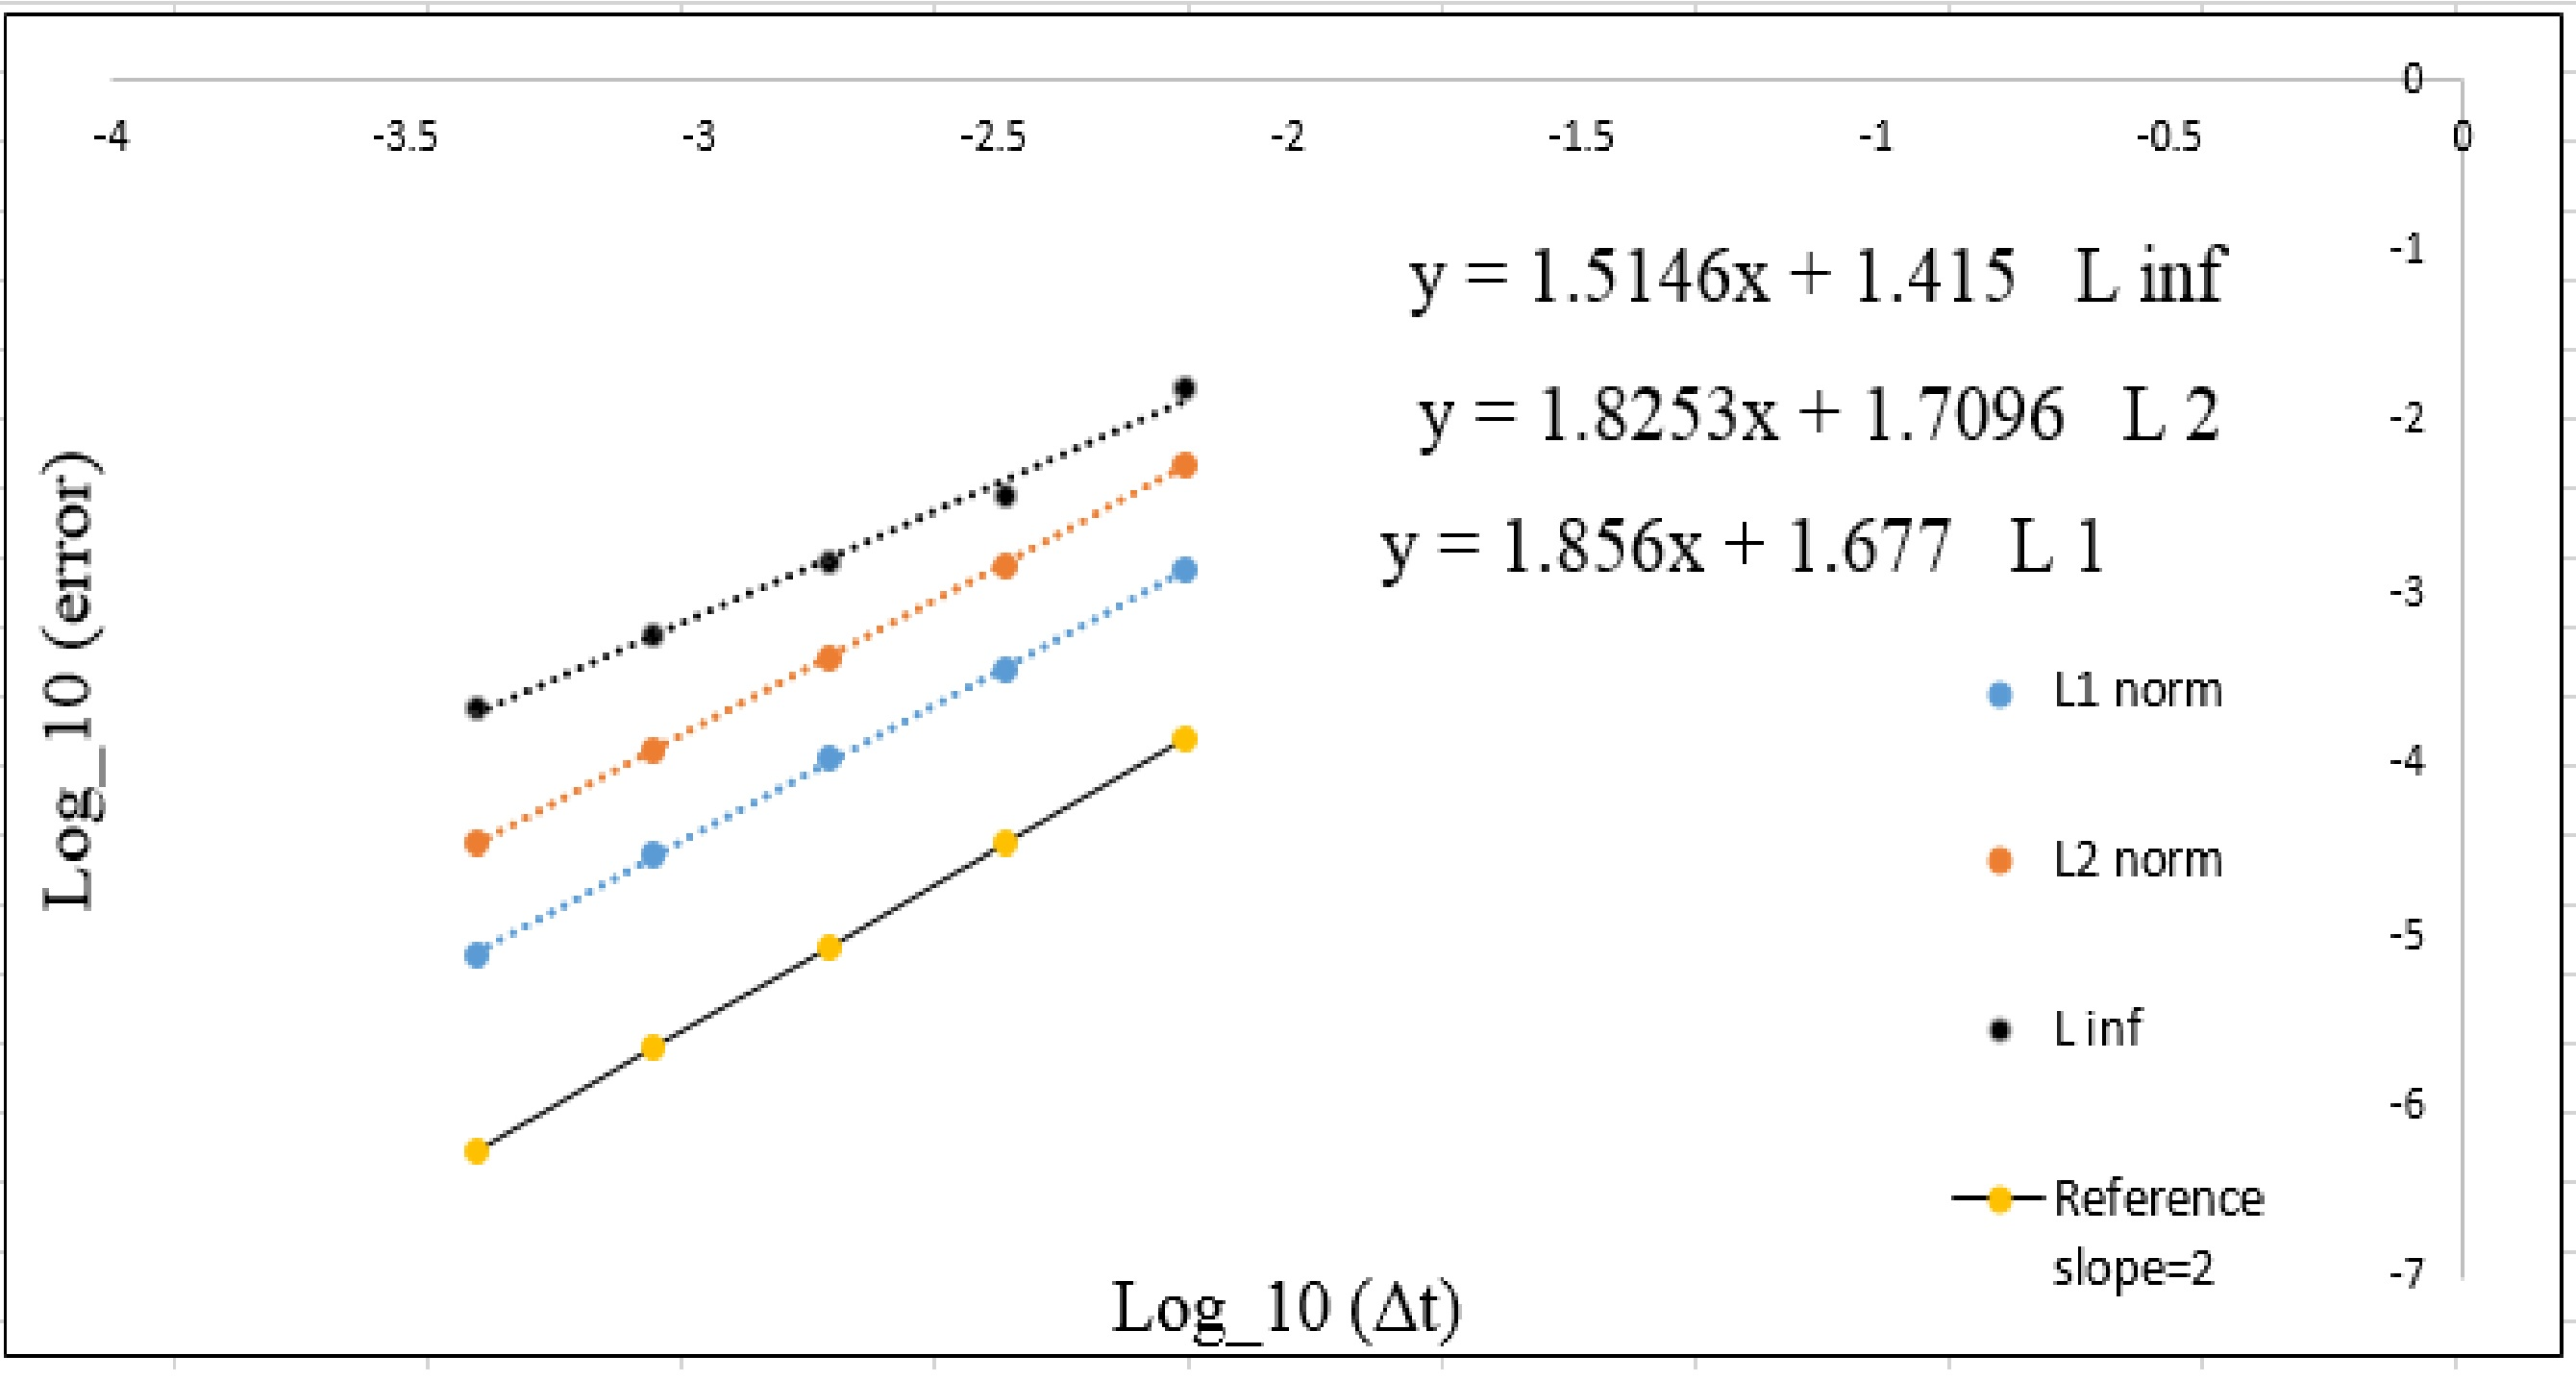
\includegraphics[width=4.5in]{figures/Pm1b_pf2b_np_div_uvstar_rate_c_0_5.jpg}}
		\caption{Log-Log plot of Convergence rate for $\nabla \cdot \textbf{u}^*$. }\label{fig:6.19b}
	\end{subfigure}
	\caption{Plot of Convergence rates for Alg 2. Domain:  $[-\dfrac{1}{2}, \dfrac{1}{2}]^2$, time = 1 and CFL = 0.5. In each plot, the data points corresponding to grid sizes of 15, 30, 60, 120, 240.}\label{fig:6.16}
\end{figure}

\begin{figure}[H]
	\centering
	\begin{subfigure}[t]{4.5in}
		\centering
		\scalebox{1.2}{
		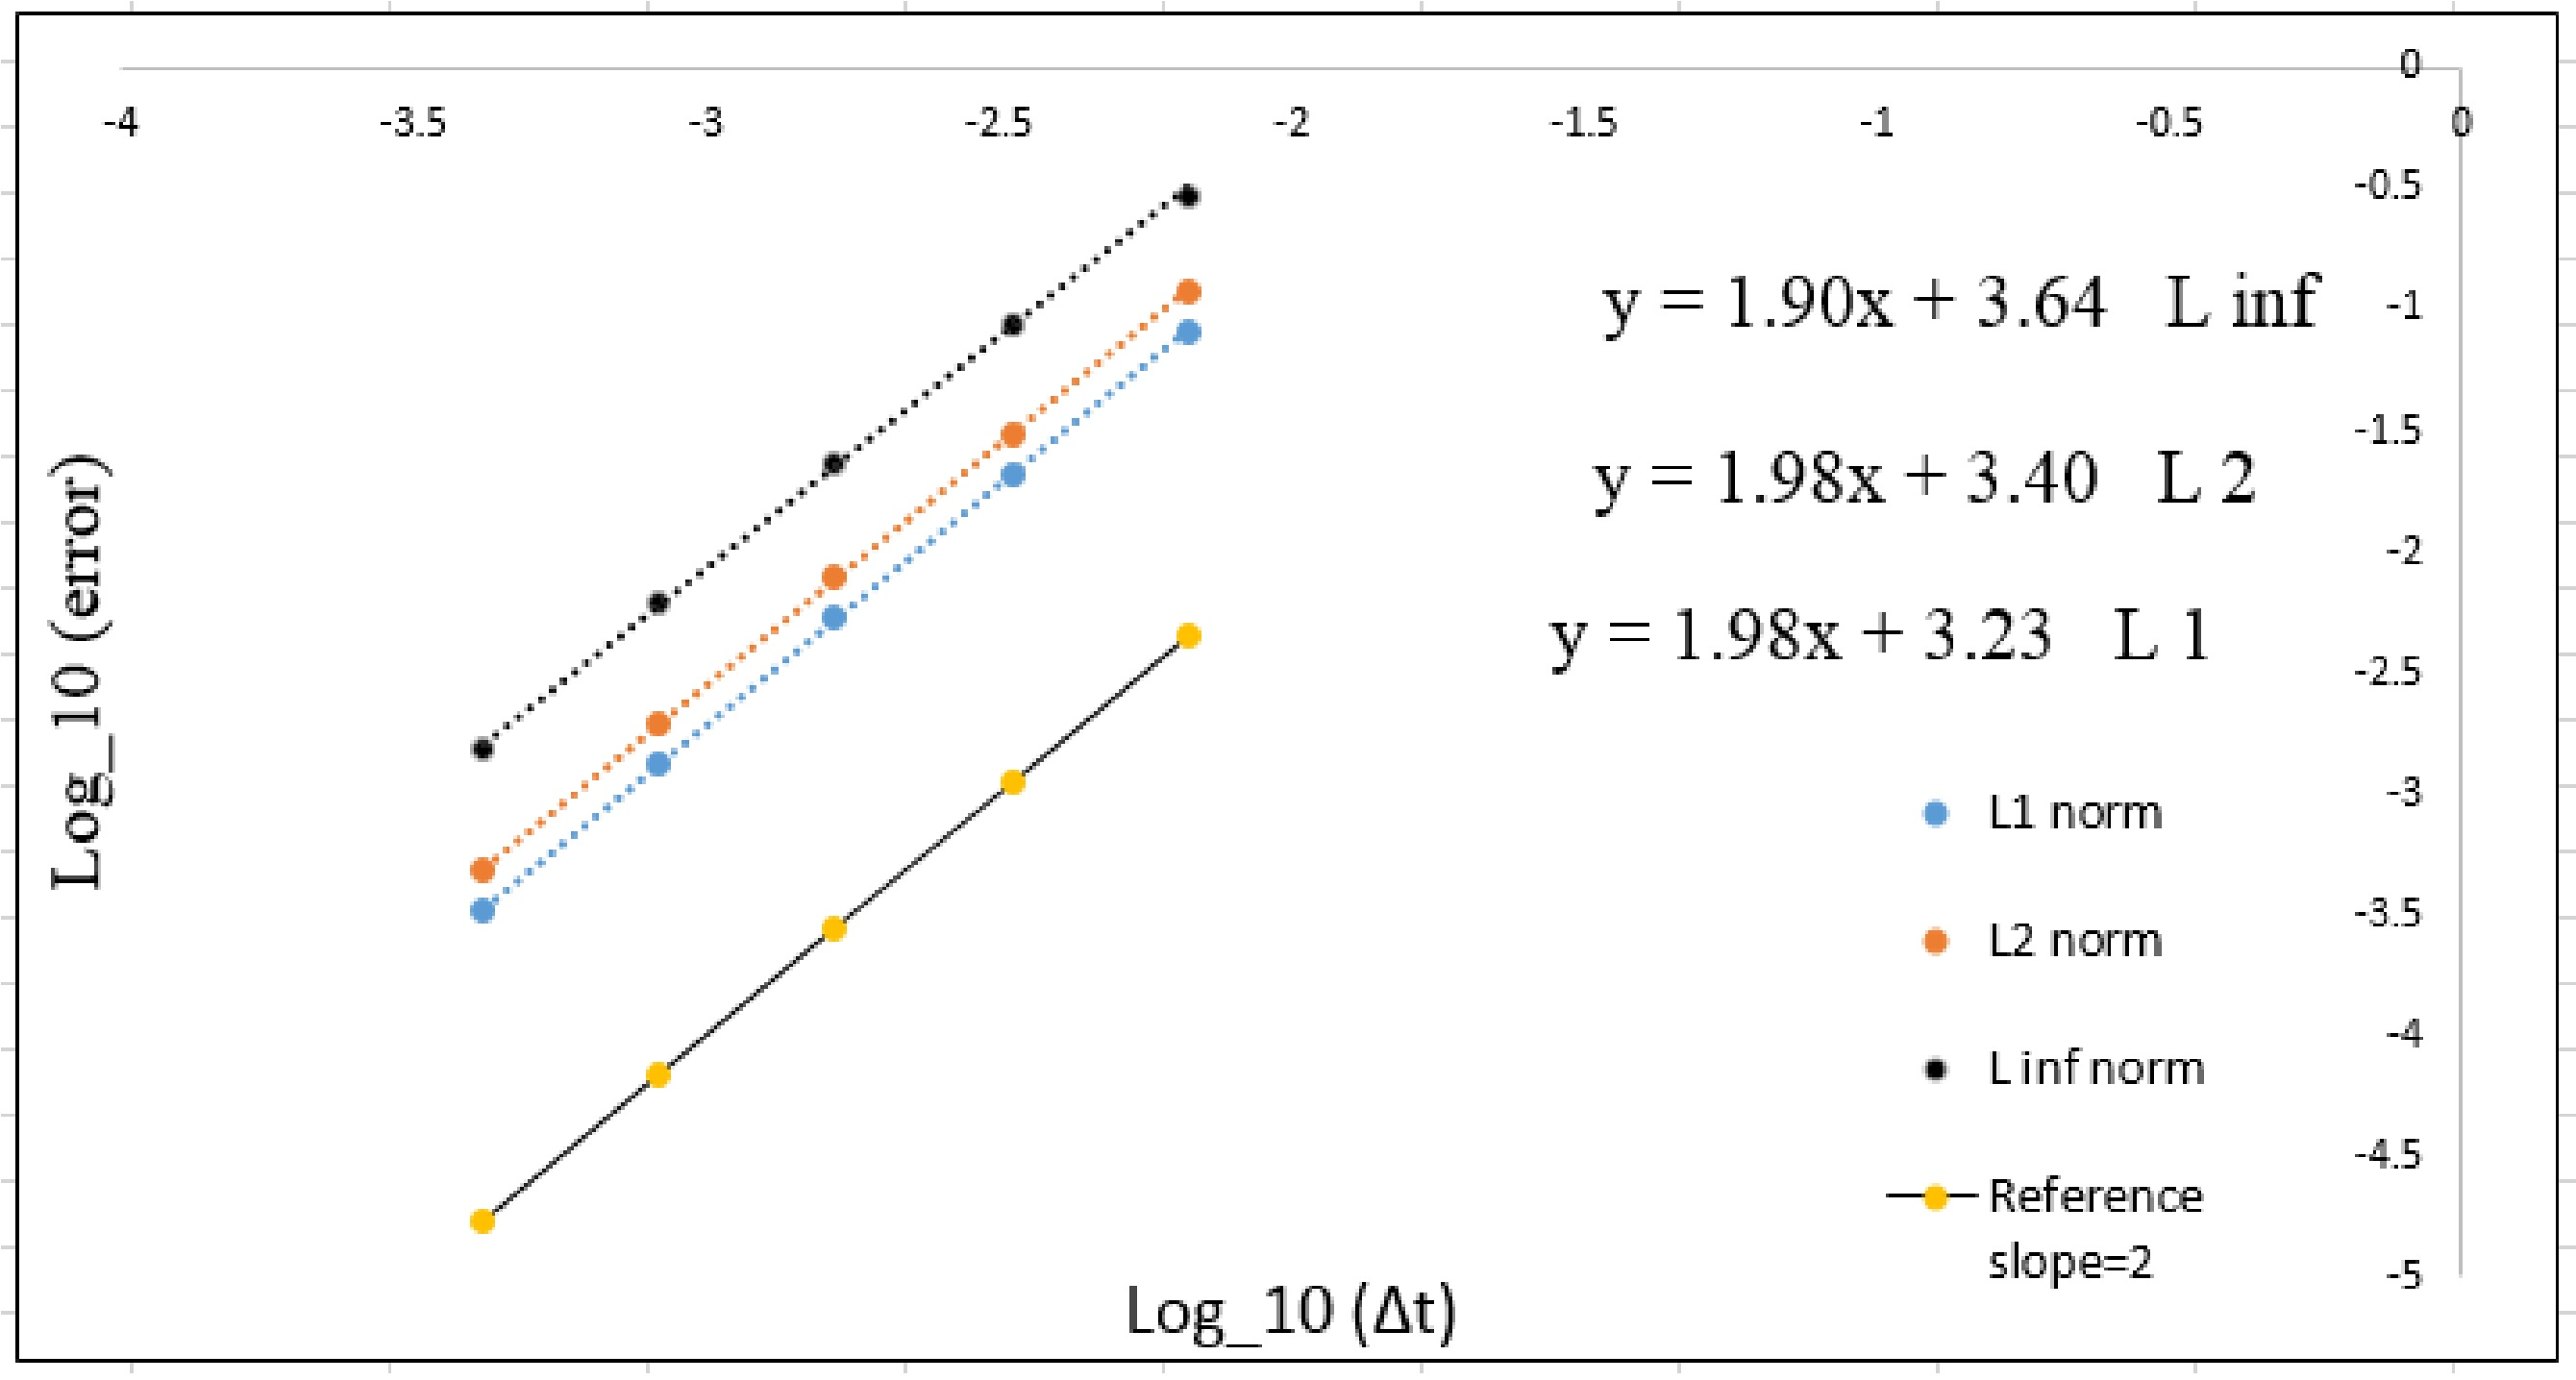
\includegraphics[width=4.5in]{figures/Pm2_pf2b_np_P_rate_c_0_5.jpg}}
		\caption{Log-Log plot of Convergence rate for Pressure}\label{fig:6.19a}		
	\end{subfigure}
	\quad
	\begin{subfigure}[t]{4.5in}
		\centering
		\scalebox{1.2}{
		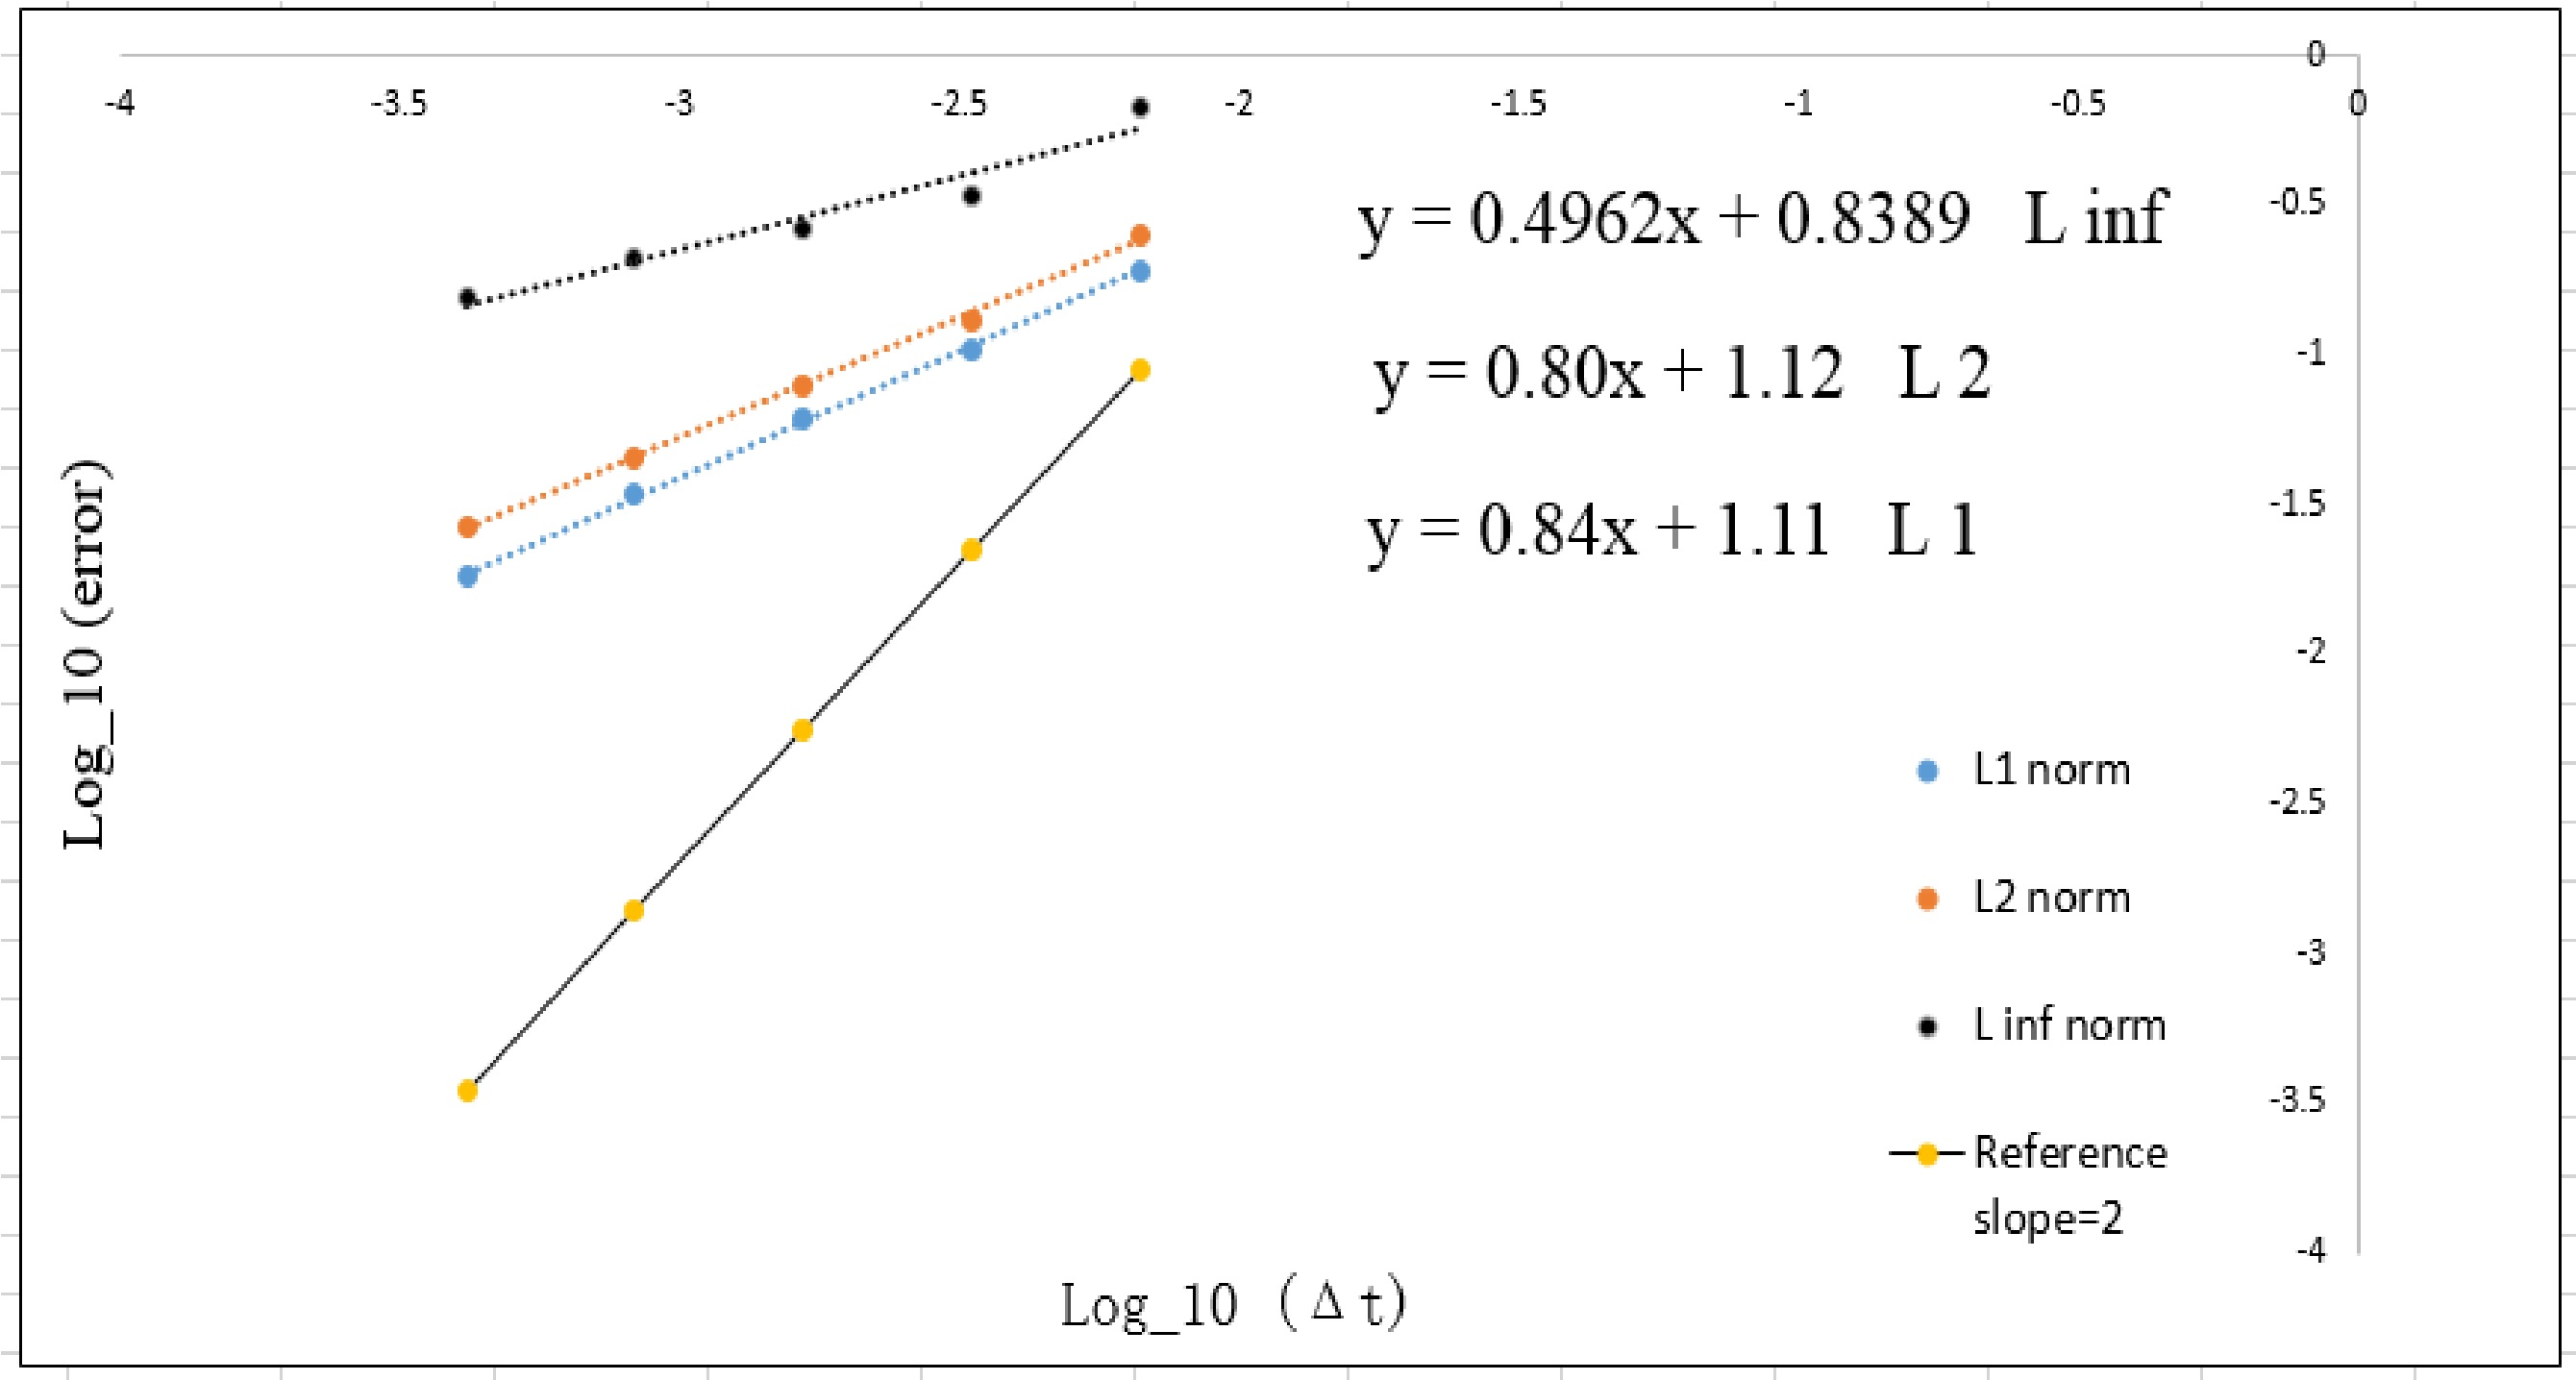
\includegraphics[width=4.5in]{figures/Pm2_pf2b_np_div_uvstar_rate_c_0_5.jpg}}
		\caption{Log-Log plot of Convergence rate for $\nabla \cdot \textbf{u}^*$. }\label{fig:6.19b}
	\end{subfigure}
	\caption{Plot of Convergence rates for Alg 3. Domain: $[-\dfrac{1}{2}, \dfrac{1}{2}]^2$, time = 1 and CFL = 0.5. In each plot, the data points corresponding to grid sizes of 15, 30, 60, 120, 240.}\label{fig:6.16}
\end{figure}

\begin{figure}[H]
	\centering
	\scalebox{1.2}{
	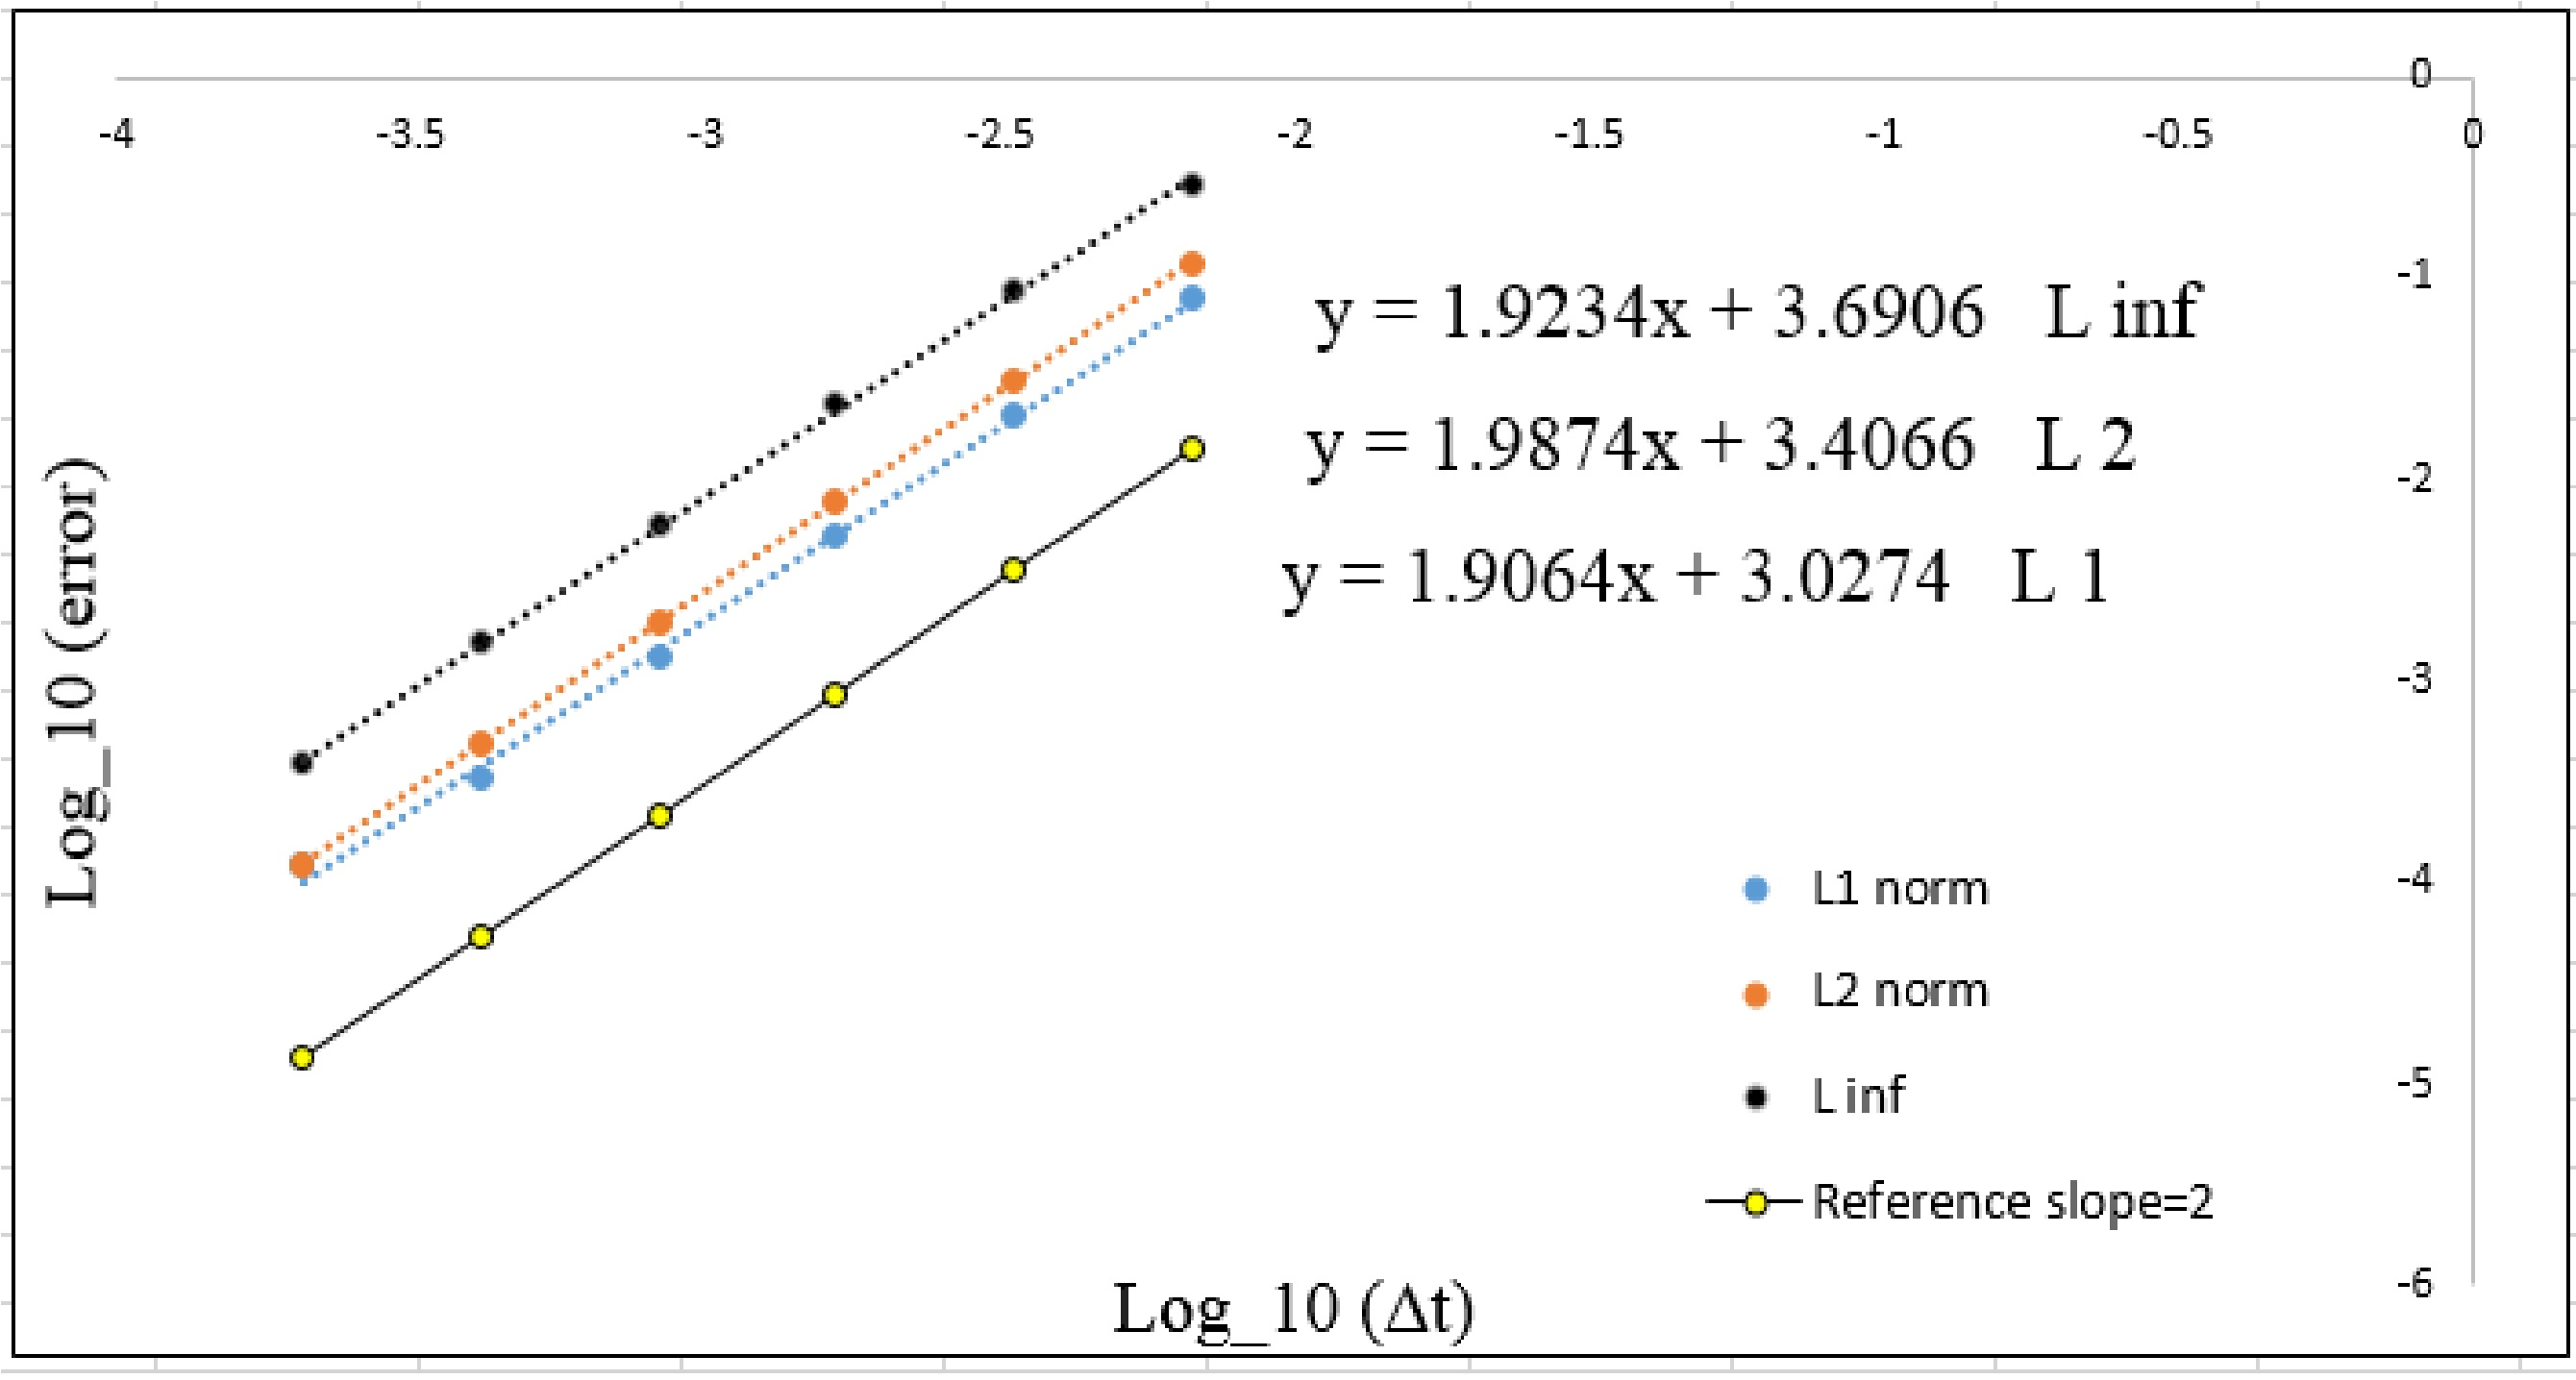
\includegraphics[width=4.5in]{figures/Gauge_pf2b_np_P_rate_c_0_5.jpg}}
	\caption{Long-Log plot of Pressure Convergence rates for Gauge method. Domain: $[-\dfrac{1}{2},\dfrac{1}{2}]^2$, time = 1 and CFL = 0.5. The data points corresponding to grid sizes of 15, 30, 60, 120, 240, and 480.}\label{fig:6.16}
\end{figure}

\begin{figure}[H]
	\centering
	\begin{subfigure}[t]{2.2in}
		\centering
		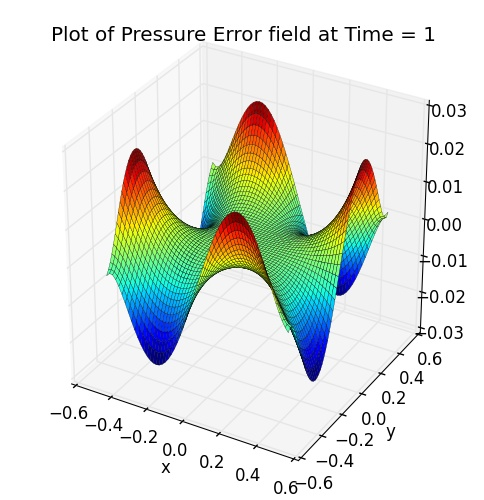
\includegraphics[width=2.2in]{figures/Pm1b_pf2b_P_error_t_1_grid_60.jpg}
		\caption{Pressure error field for Alg 2 method}\label{fig:6.19a}		
	\end{subfigure}
	\quad
	\begin{subfigure}[t]{2.6in}
		\centering
		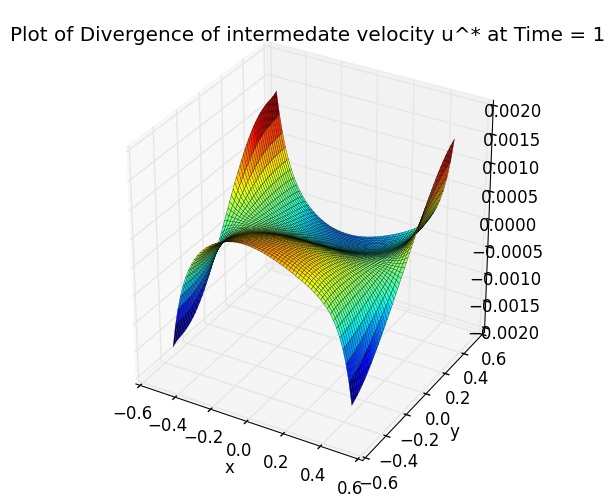
\includegraphics[width=2.6in]{figures/Pm1b_pf2b_div_uvstar_t_1_grid_60.jpg}
		\caption{Divergence of intermediate velocity field for Alg 2 method. }\label{fig:6.19b}
	\end{subfigure}
	\quad
	\centering
	\begin{subfigure}[t]{2.2in}
		\centering
		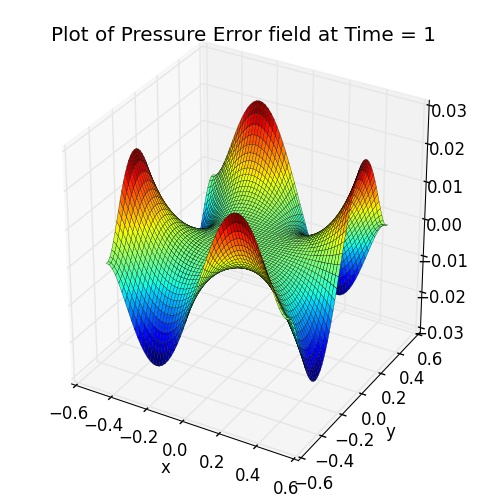
\includegraphics[width=2.2in]{figures/Pm2_pf2b_np_P_error_t_1_grid_60.jpg}
		\caption{Pressure error field for Alg 3 method}\label{fig:6.19c}		
	\end{subfigure}
	\quad
	\begin{subfigure}[t]{2.6in}
		\centering
		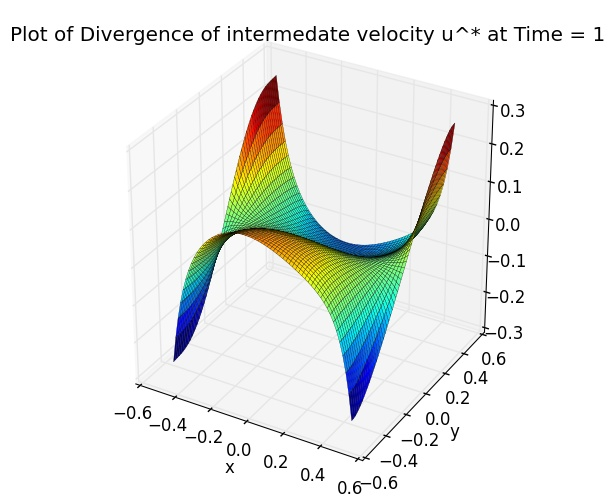
\includegraphics[width=2.6in]{figures/Pm2_pf2b_np_div_uvstar_t_1_grid_60.jpg}
		\caption{Divergence of intermediate velocity field for Alg 3 method.}\label{fig:6.19d}
	\end{subfigure}
	\quad
	\begin{subfigure}[t]{2.5in}
		\centering
		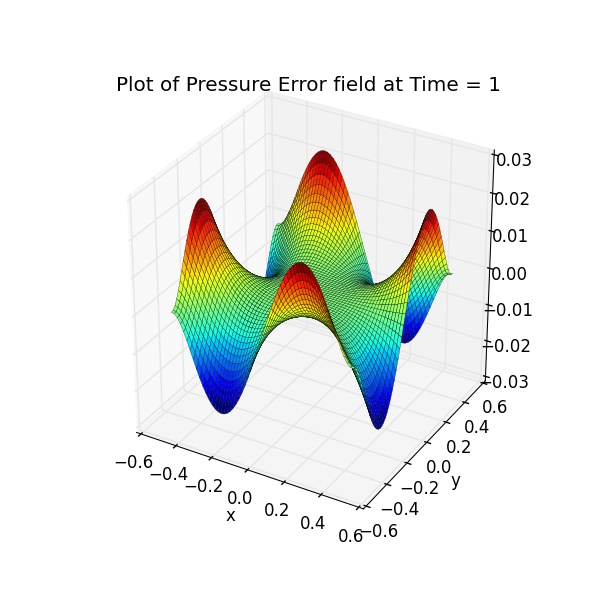
\includegraphics[width=2.5in]{figures/Gauge_pf2b_P_error_t_1_grid_60_corrected.jpg}
		\caption{Pressure error field for Gauge method. }\label{fig:6.19d}
	\end{subfigure}
	\caption{Pressure error fields and divergence of intermediate velocity (if applicable) for Alg 2, Alg 3 and Gauge method at grid size of 120. Domain: $[-\dfrac{1}{2},\dfrac{1}{2}]^2$, time = 1 and CFL = 0.5. }\label{fig:6.16}
\end{figure}

\subsection*{Necessity for accurate approximation to $\phi^{n+1}$ along the tangential boundary of the intermediate velocity field.}
We investigate the importance of boundary condition choice for the intermediate velocity field and this might also help to understand why Alg 3 behaves better than Alg 2 in pressure convergence rates. We took two extrema here in choosing the tangential boundary condition for $\textbf{u}^*$: one is use second order approximation to $\phi^{n+1}$ so we have $\textbf{$\tau$} \cdot \textbf{u}^* \,|_{\partial \Omega} = \textbf{$\tau$} \cdot (\textbf{u}^{n+1} + \nabla (2\phi^n - \phi^{n-1})\,|_{\partial \Omega}$ (as of what we have done before for Alg 3); the other is to use no approximation to $\phi^{n+1}$. We now rerun Alg 3 with the less accurate boundary where $\textbf{$\tau$} \cdot \textbf{u}^* = \textbf{$\tau$} \cdot \textbf{u}^{n+1}$ (this is the same as Alg 2). The convergence rates in pressure are again summarised in Figure below. It is observed that the rates are much reduced to about 0.7 order. The plot of pressure error field also shows four spikes at corners as in Alg 2. Hence this indicate the choice of tangential boundary condition to $\textbf{u}^*$ does indeed affect the performance of numerical boundary layer elimination. This finding indicates that for Alg 3 accurate approximation to $\phi^{n+1}$ must be implemented when computing the intermediate velocity field along the boundary points. This is consistent with the predications of our normal mode analysis. It is also consistent with the findings of others \cite{brown2001accurate}. We infer that the same result might also work for Alg 2. However we did not have enough time to implement the different condition for Alg 2.

\begin{figure}[H]
	\centering
	\scalebox{1.5}{
	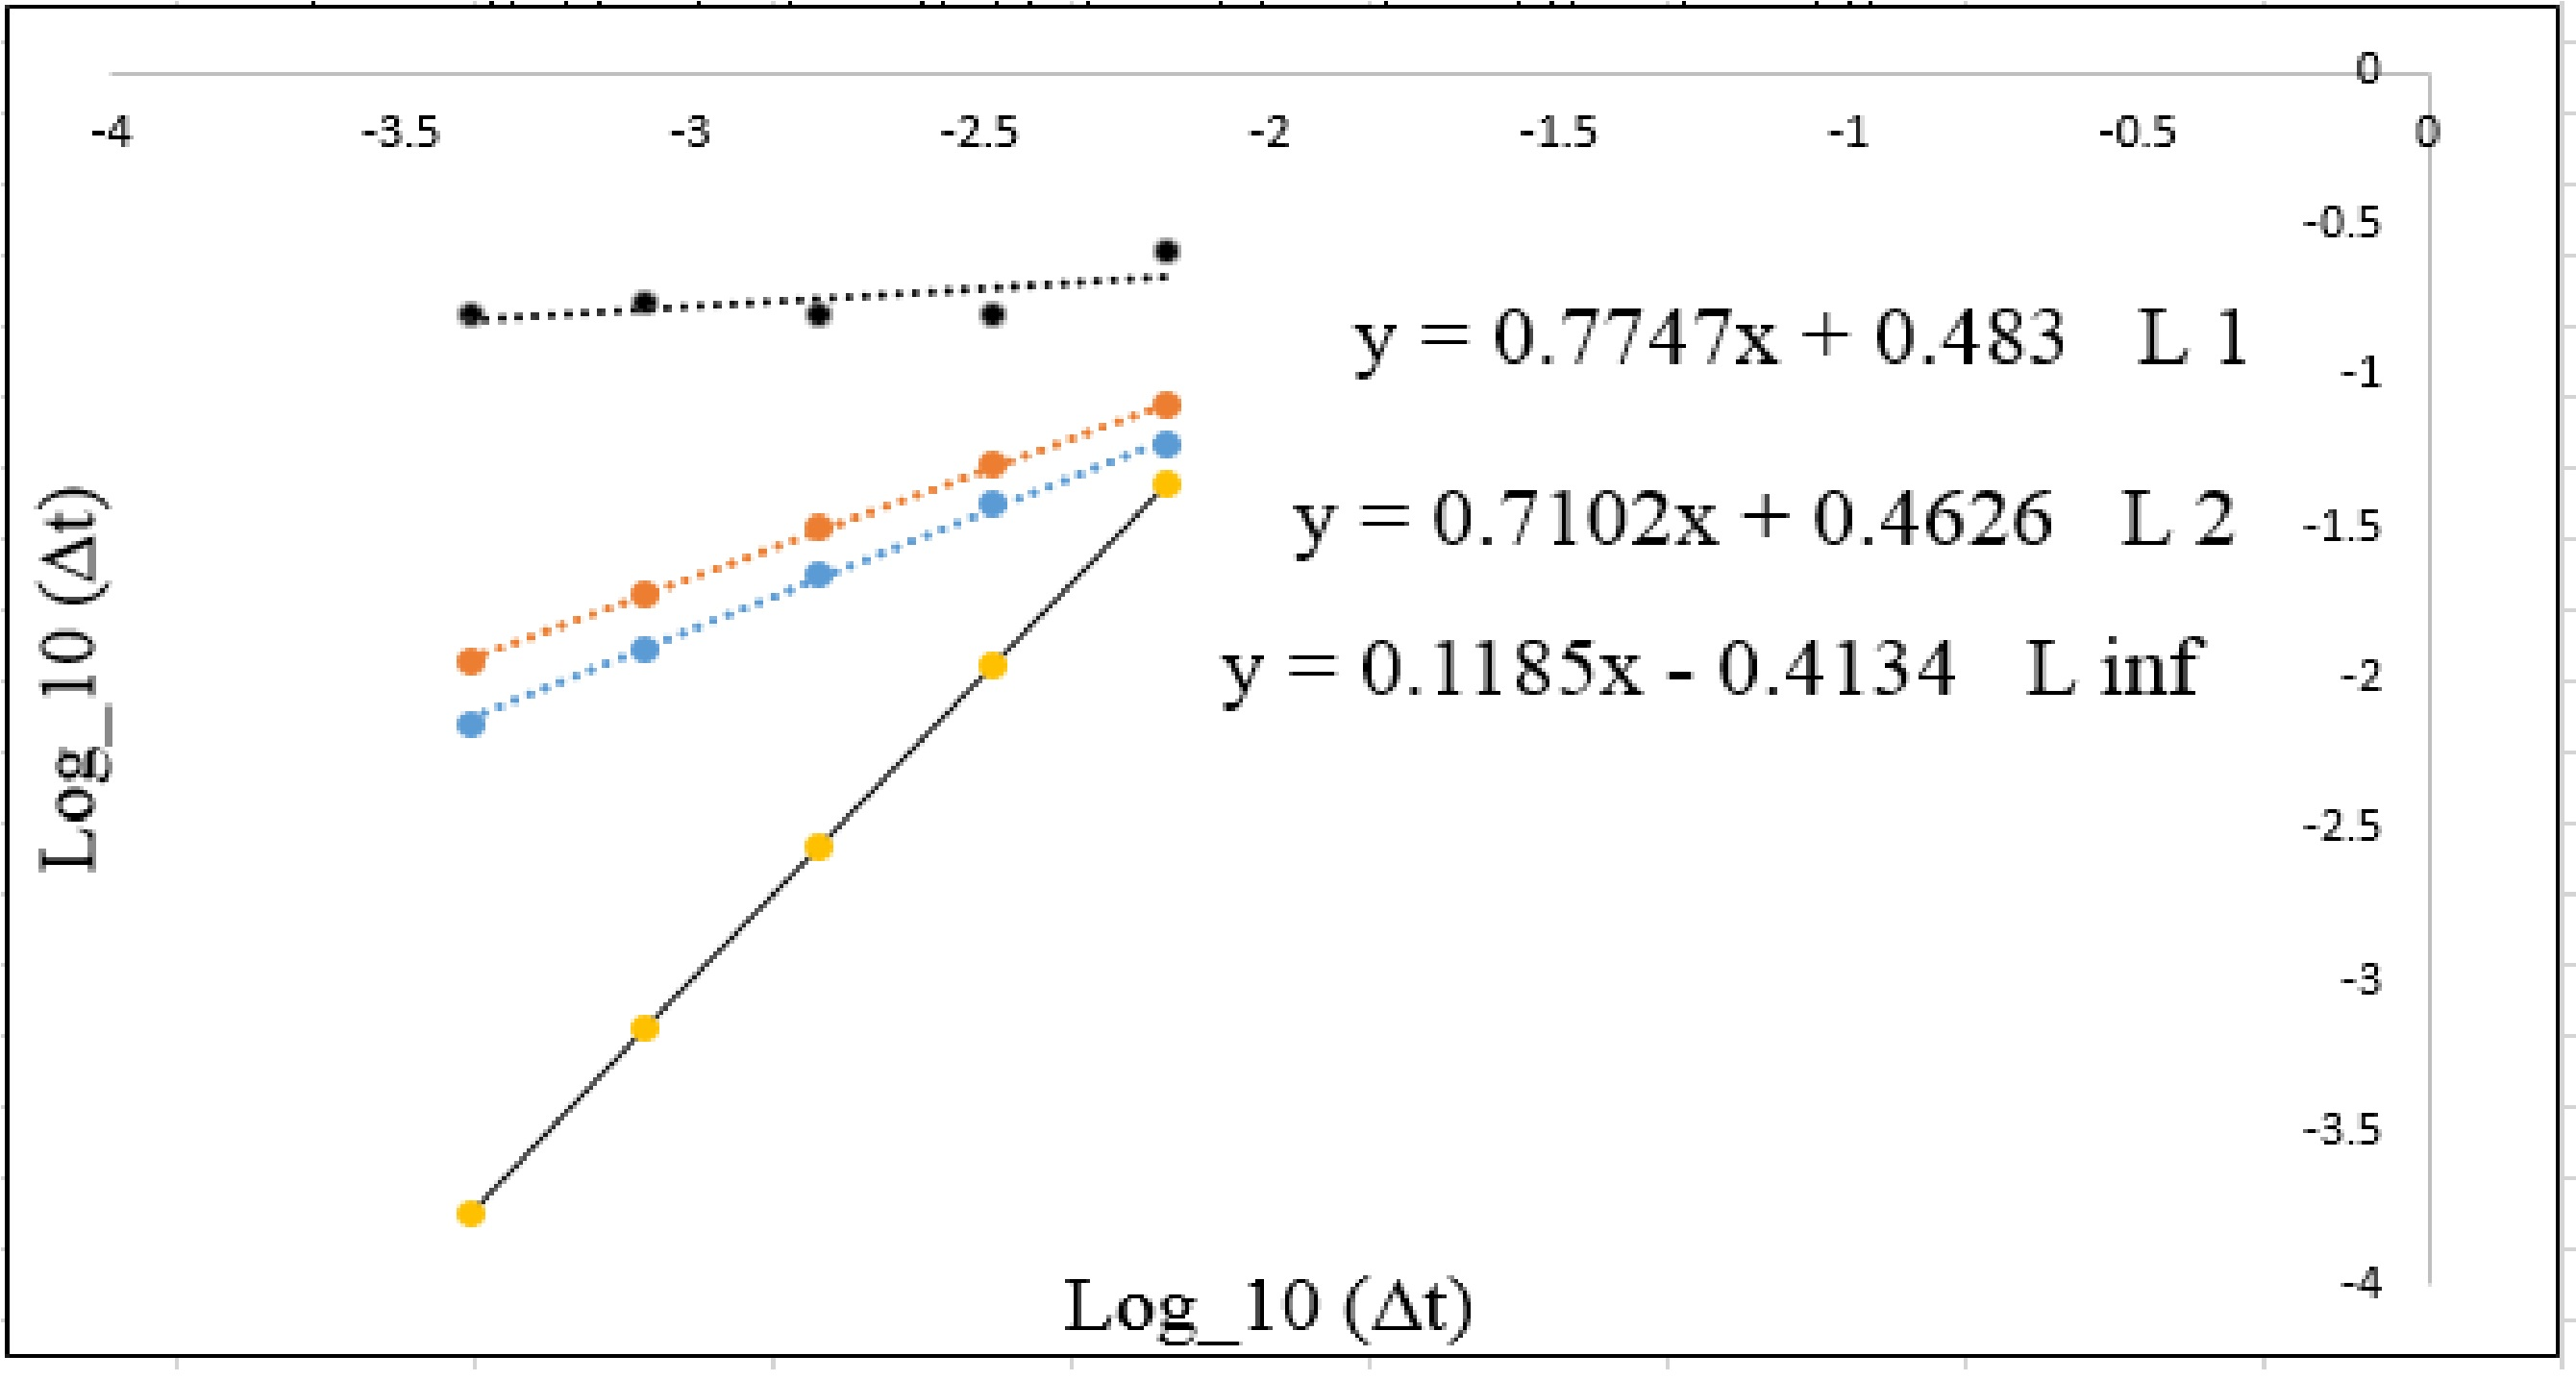
\includegraphics[width=3.5in]{figures/Pm2D_pf2_p_rate_cfl_0_5.jpg}}
	\caption{Log log plot of pressure error convergence rate for Alg 3 with less accurate boundary condition for $\nabla \cdot \textbf{u}^*$. }\label{fig:6.20}
\end{figure}
	
\begin{figure}[H]
	\begin{subfigure}[t]{2.6in}
		\centering
		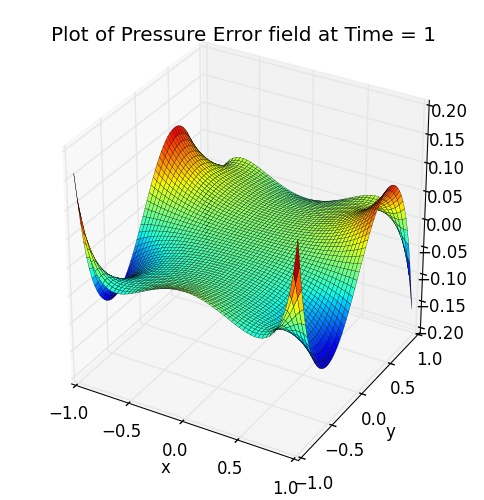
\includegraphics[width=2.6in]{figures/Pm2D_pf2_np_P_error_t_1_grid_60.jpg}
		\caption{Pressure error field for Alg 3 with grid size 60 at time 1. }\label{fig:6.19b}
	\end{subfigure}
	\begin{subfigure}[t]{3.0in}
		\centering
		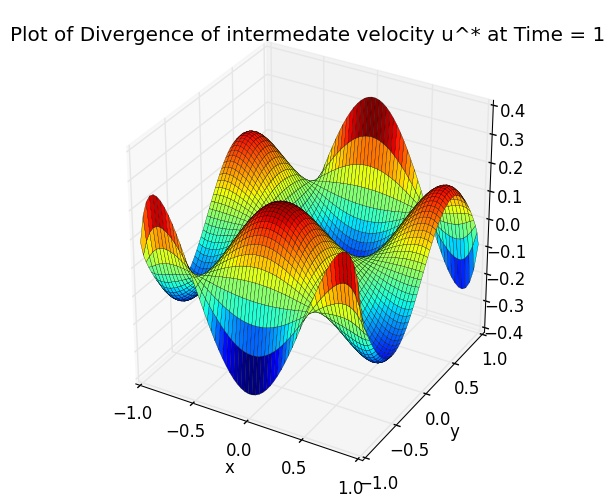
\includegraphics[width=3.0in]{figures/Pm2D_pf2_np_div_uvstar_t_1_grid_60.jpg}
		\caption{Plot of $\nabla \cdot \textbf{u}^*$ for Alg 3 with grid size 60 at time 1. }\label{fig:6.19b}
	\end{subfigure}
	\caption{Long-Log plot of Pressure Convergence rates and $3D$ surface plot of pressure error field for Alg 3 where the less accurate tangential boundary is used. Domain: $[-1,1]^2$, time = 1 and CFL = 0.5. The data points corresponding to grid sizes of 15, 30, 60, 120, 240.}\label{fig:6.19c}
\end{figure}

\newpage
\subsection{Unforced flow problem}

To test the effect of smoothness of domain to the accuracy of projection methods. Another unforced flow problem is also considered. It is the well-known 2-D Taylor solution to the Navier Stokes equations. The analytic solutions are:

\begin{dgroup}
\begin{dmath}
u = -\cos(x)\sin(y)e^{-2t}
\end{dmath}
\begin{dmath}
v = \sin(x)\cos(y)e^{-2t}
\end{dmath}
\begin{dmath}
p = -\dfrac{1}{4\,R}(\cos(2x)+\cos(2y))e^{-4t}
\end{dmath}
\end{dgroup}

This test problem has non-zero boundary conditions for velocities and non-zero pressure gradients, unlike the forced flow exampled we have considered before where 2 of its boundaries are zero for velocities and pressure. Hence this should reveal more information on how the projection methods depends on the structure of domain and boundary conditions. For simplicity let's consider the domain: $[-\dfrac{\pi}{4}, \dfrac{\pi}{4}]^2$. Then the pressure value at these 4 corners ($x = \pm \dfrac{\pi}{4}$ and $y = \pm \dfrac{\pi}{4}$) would then be zero for all times which makes our pressure normalisation process easier.\\

In addition, this Taylor solutions are derived from the full Navier Stokes equations and hence it is also good to test our convective term solvers too.\\

We have again run the Projection methods and Gauge for 5 grid sizes from $15 \times 15$ to $240 \times 240$. The spatial stepping is halved each time. The solutions are calculated at time 1s and with Reynolds number equals to 1. A CFL number of 0.5 is used in all methods to obtain better error estimates.\\

The convergence rates in pressure are summarised in Figure. Interestingly all the methods show fully second order convergence except for Alg 2 where only first order convergence is observed. This time all the norms show degraded accuracy. Take a look at the Pressure error field we observe very large spikes located at the 4 corners of the domain. This indicates the Presence of numerical boundary layers which are manifested better in the plot of Divergence of intermediate velocity field. Interestingly the magnitude of divergence of numerical boundary in intermediate velocity field is even larger for Alg 3 yet resulting in small Pressure error field. This result shows that the numerical boundary layers in $\phi$ and $\nabla \cdot \textbf{u}^*$ cannot be fully filtered out in the projection methods unless accurate boundary condition for $\textbf{$\tau$} \cdot \textbf{u}^*$ is implemented, same finding that supports the necessity for accurate tangential boundary condition for the intermediate velocity field. This is illustrated by the surface plots in Alg 2 where the thick boundary layer in $\nabla \cdot \textbf{u}^*$ is eliminated in Pressure but the 4 spikes still present. This finding is also consistent with that obtained in David's paper \cite{brown2001accurate}.\\

\begin{figure}[H]
	\centering
	\begin{subfigure}[t]{4.5in}
		\centering
		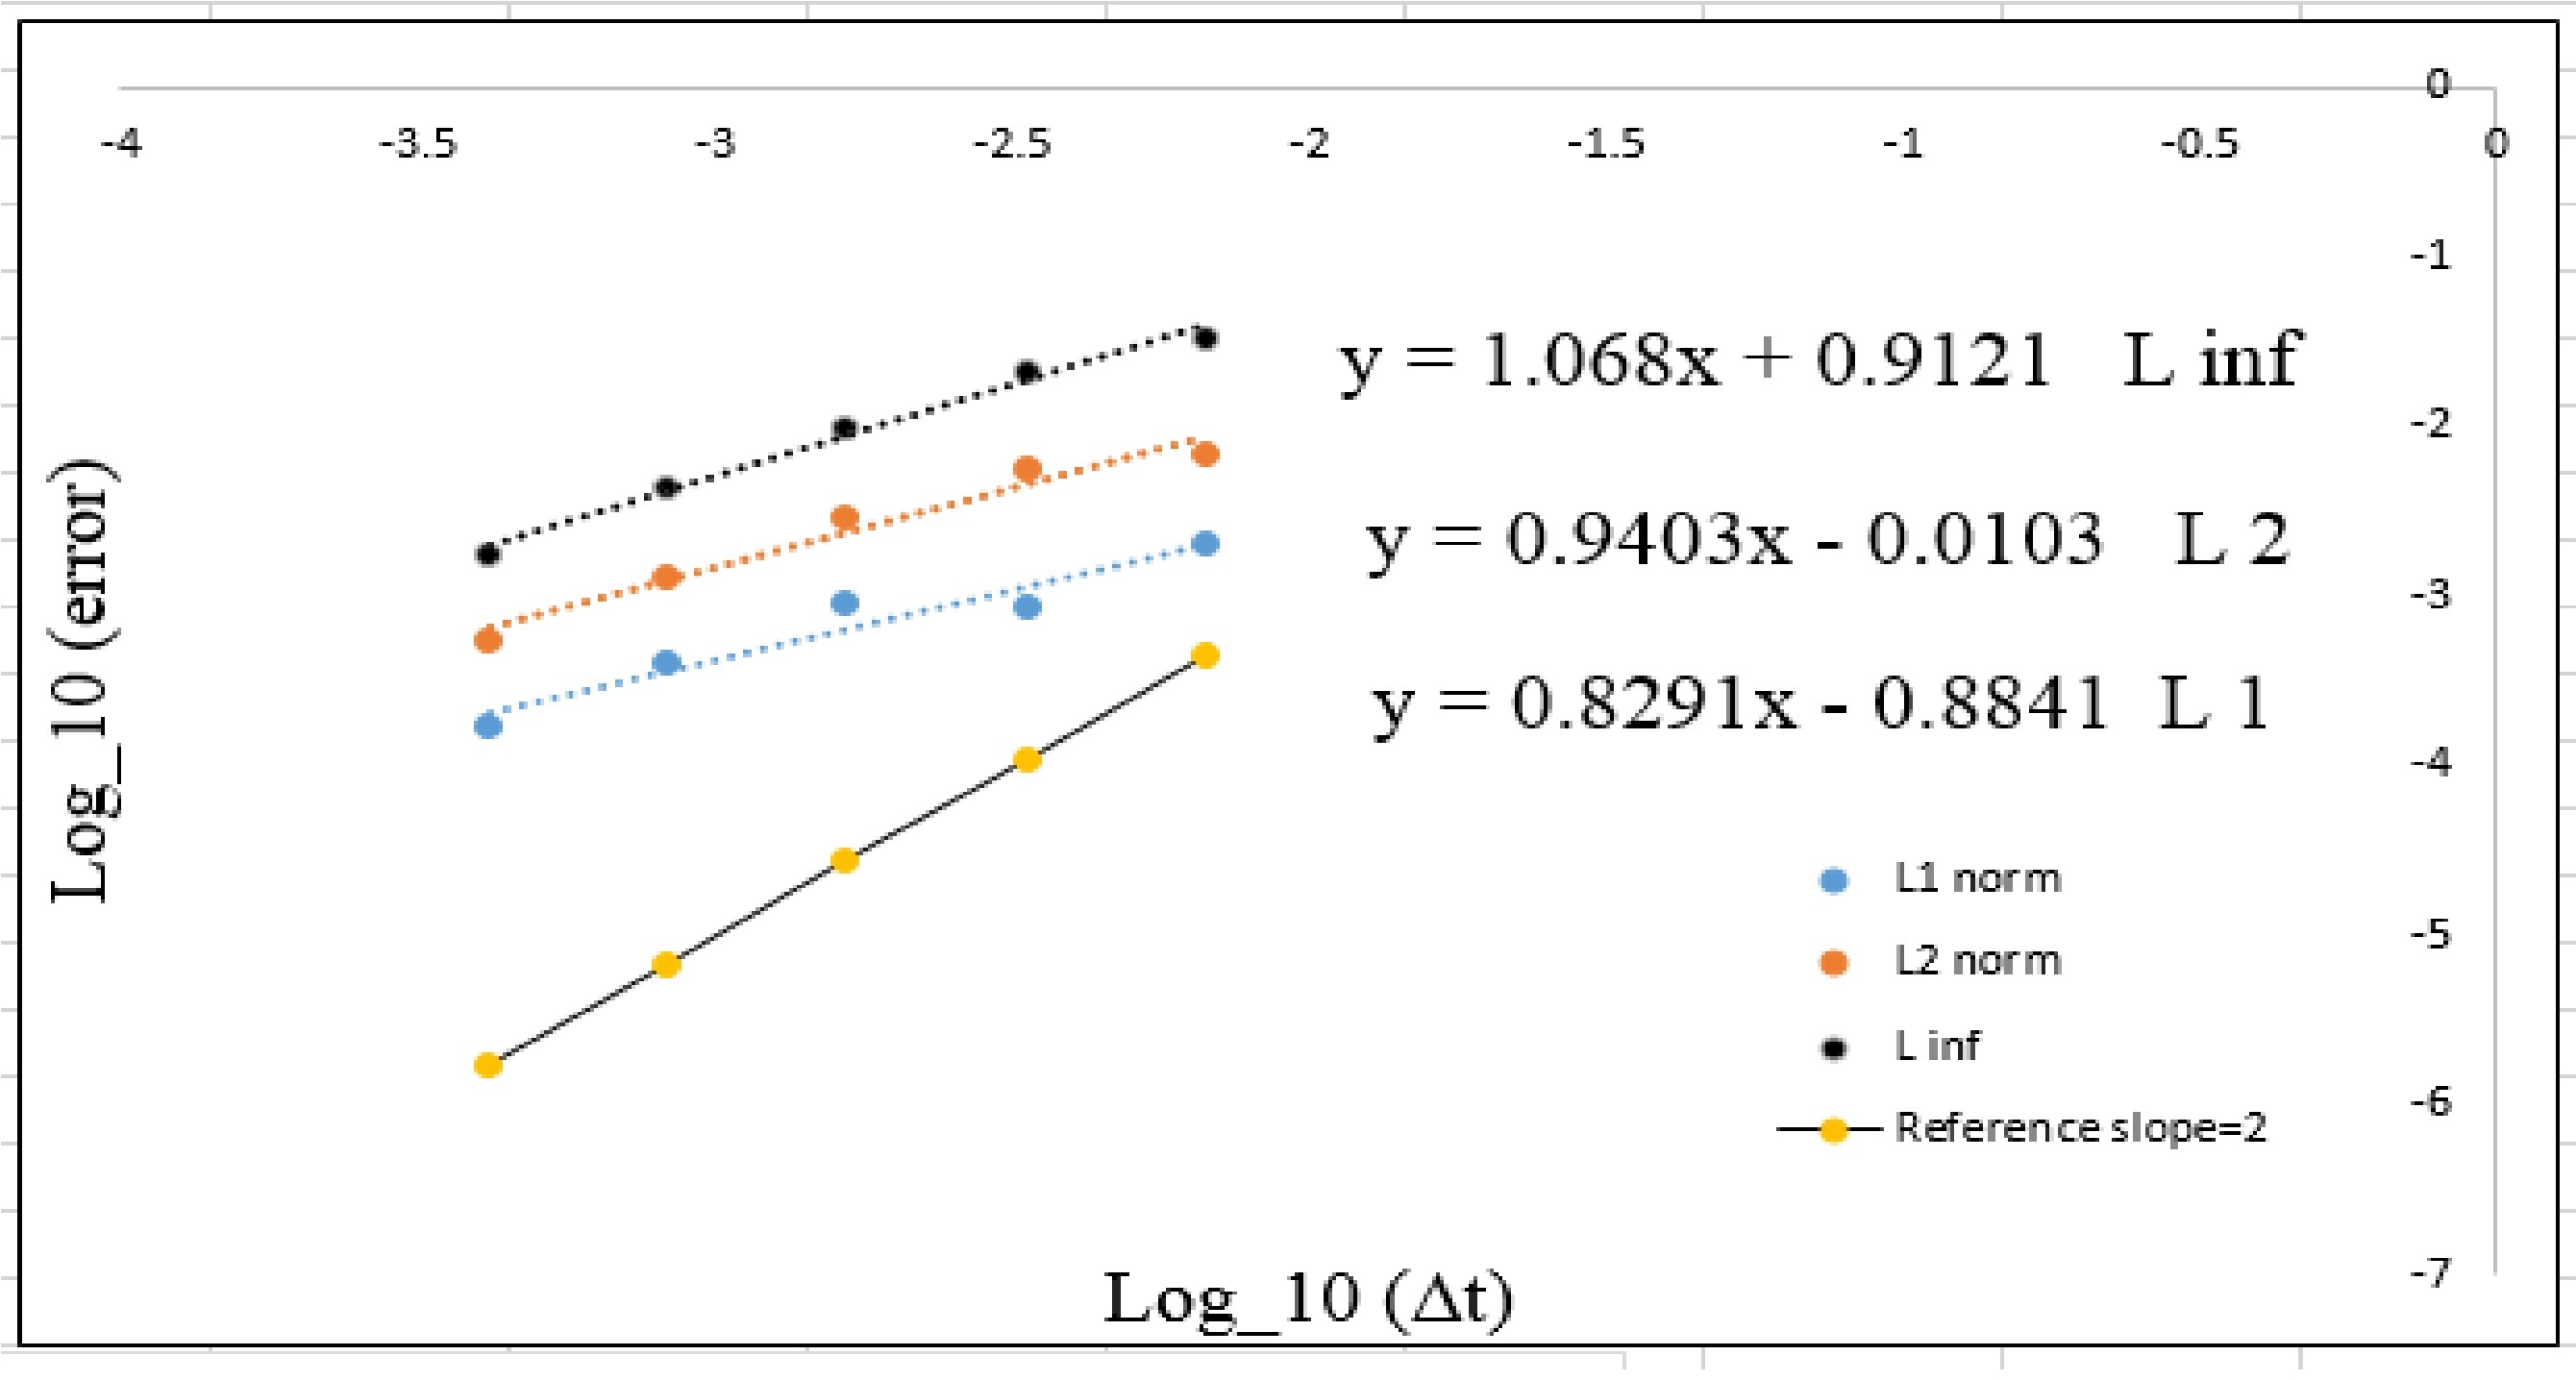
\includegraphics[width=4.5in]{figures/Pm1b_unf1_np_P_rate.jpg}
		\caption{Log-Log plot of Convergence rate for Pressure Alg 2 method}\label{fig:6.19a}		
	\end{subfigure}
	\quad
	\begin{subfigure}[t]{4.5in}
		\centering
		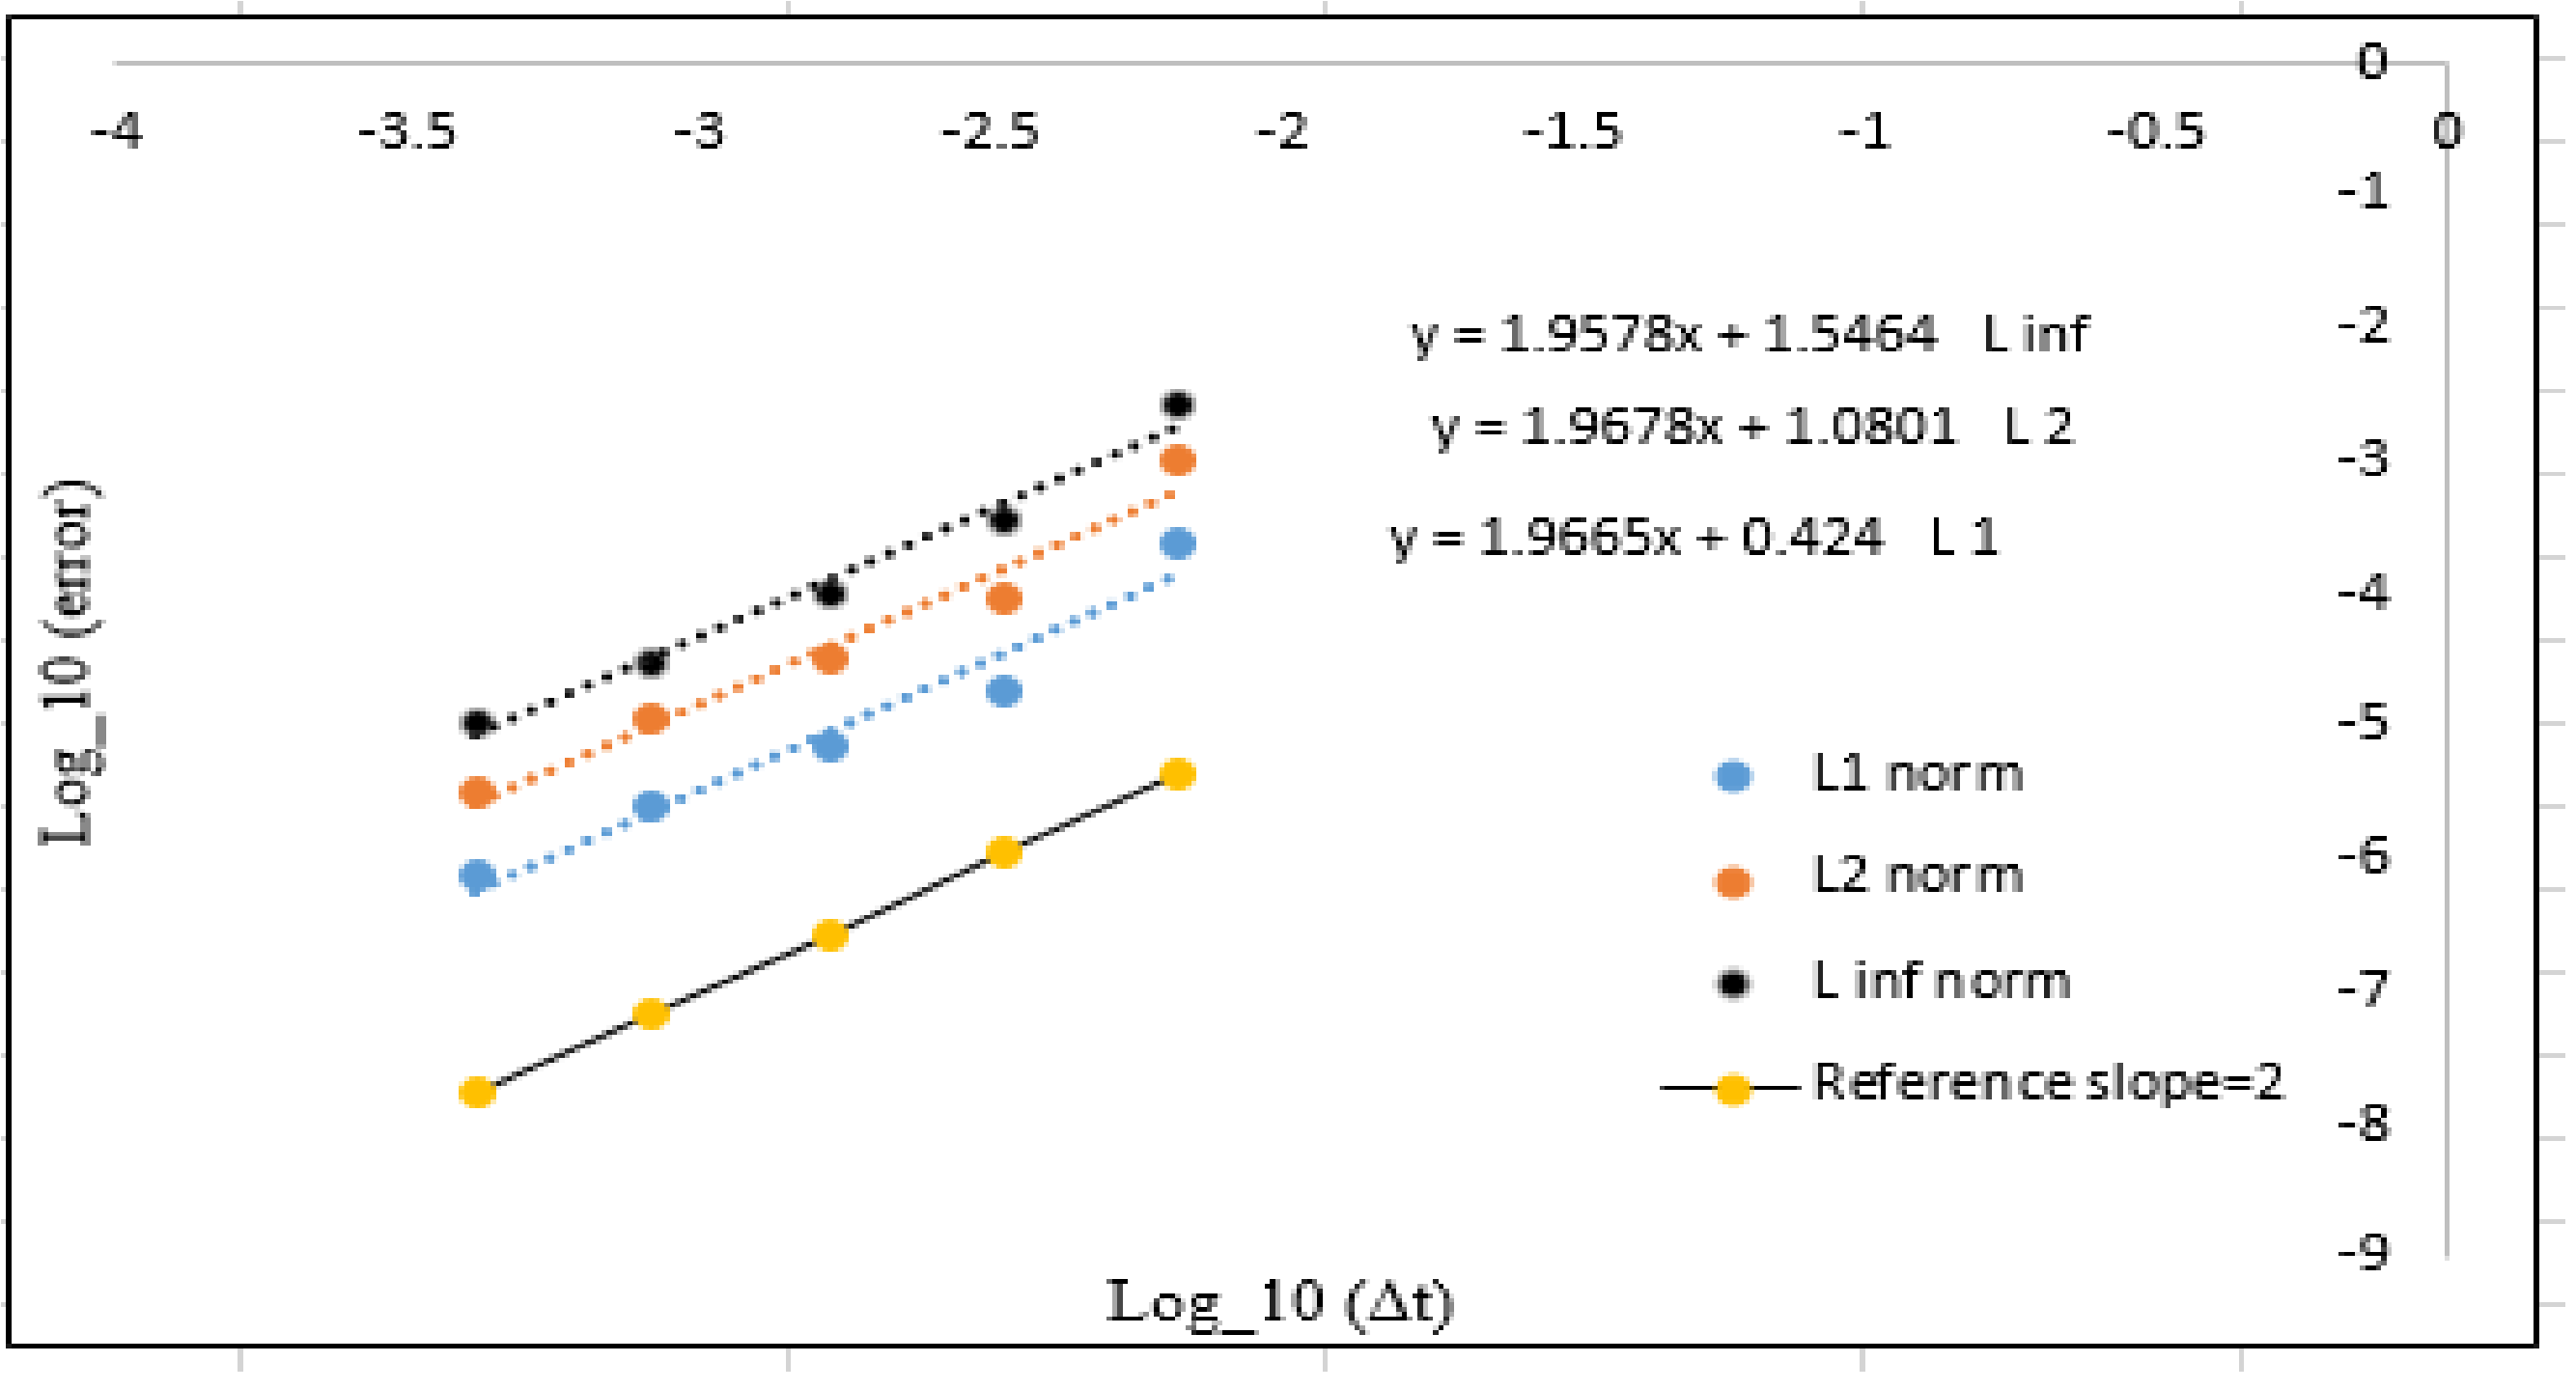
\includegraphics[width=4.5in]{figures/Pm2_unf1_np_P_rate.jpg}
		\caption{Log-Log plot of Convergence rate for Pressure Alg 3. }\label{fig:6.19b}
	\end{subfigure}
	\quad
	\begin{subfigure}[t]{4.5in}
		\centering
		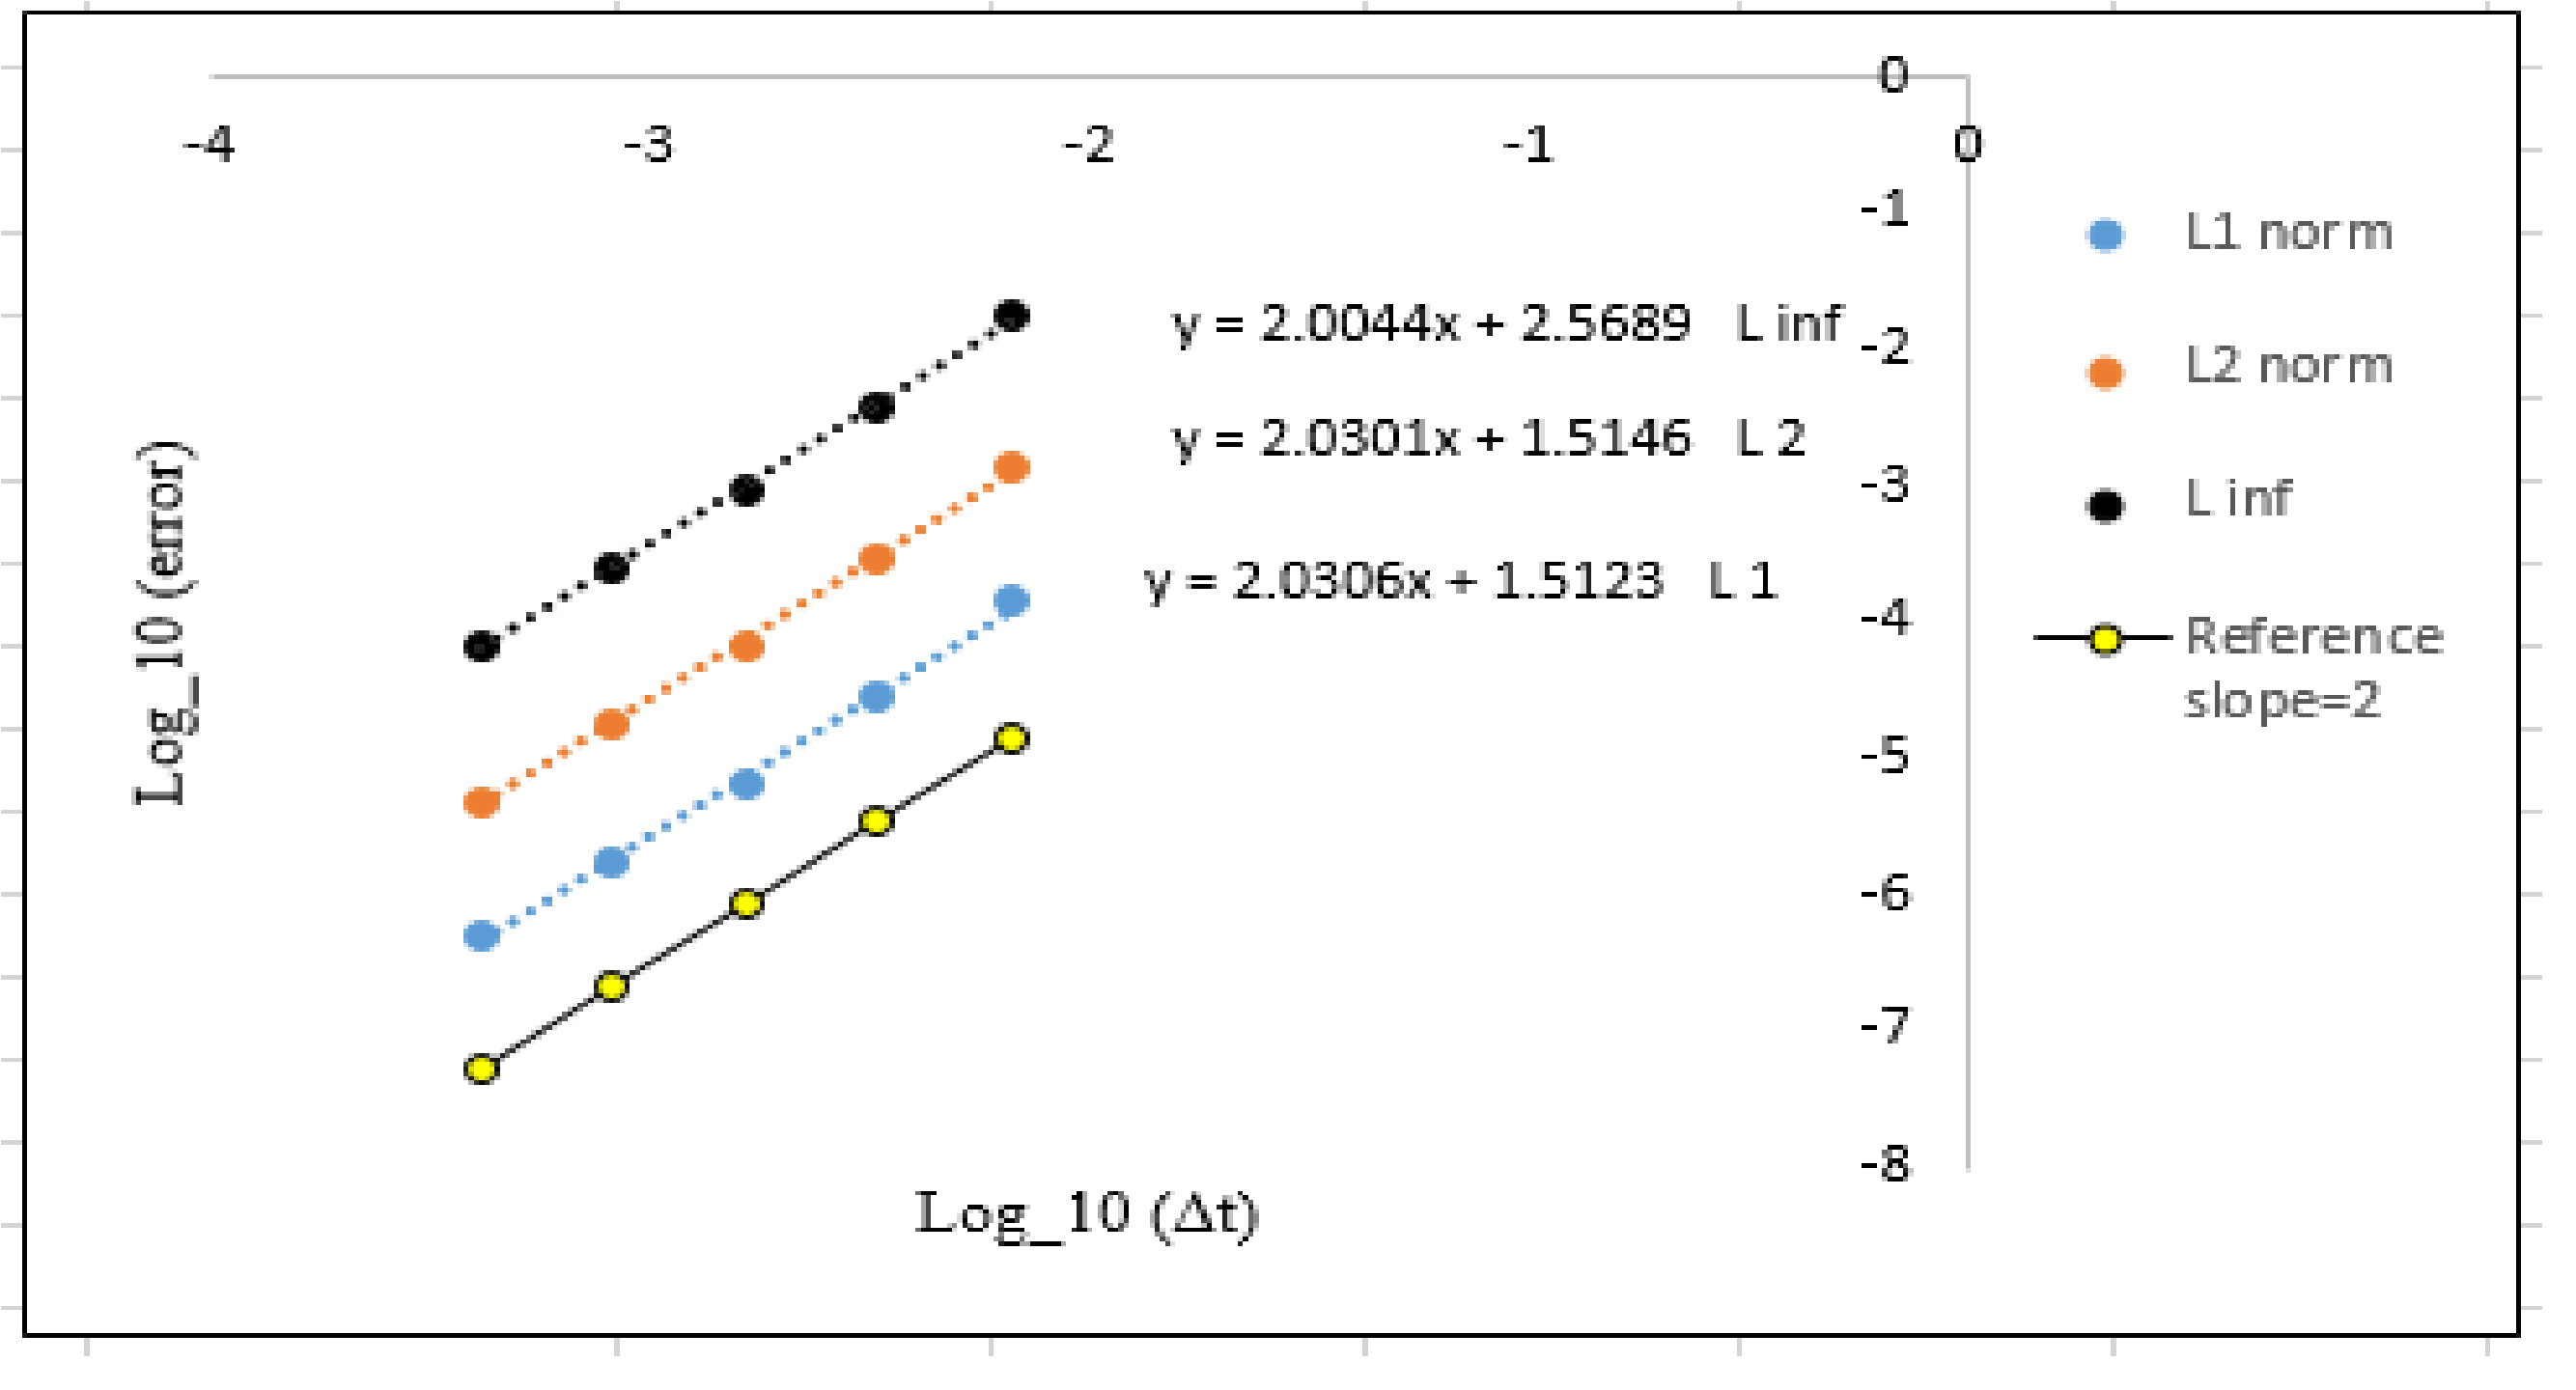
\includegraphics[width=4.5in]{figures/Gauge_unf1_np_P_rate.jpg}
		\caption{Log-Log plot of Convergence rate for Pressure Gauge method }\label{fig:6.19b}
	\end{subfigure}
	\caption{Plot of Convergence rates for the Unforced flow problem with Normalised Pressure approach used. Domain: $[-\dfrac{\pi}{4}, \dfrac{\pi}{4}]^2$, time = 1 and CFL = 0.5. In each plot, the data points corresponding to grid sizes of 15, 30, 60, 120, 240.}\label{fig:6.16}
\end{figure}

\begin{figure}[H]
	\centering
	\begin{subfigure}[t]{2.2in}
		\centering
		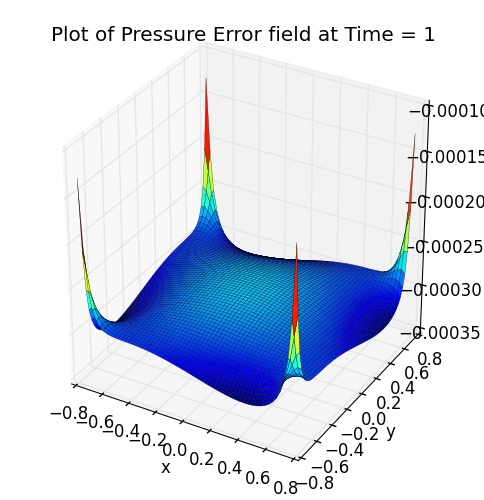
\includegraphics[width=2.2in]{figures/Pm1b_unf1_np_P_error_t_1_grid_60.jpg}
		\caption{Pressure error field for Alg 2 method}\label{fig:6.19a}		
	\end{subfigure}
	\quad
	\begin{subfigure}[t]{2.6in}
		\centering
		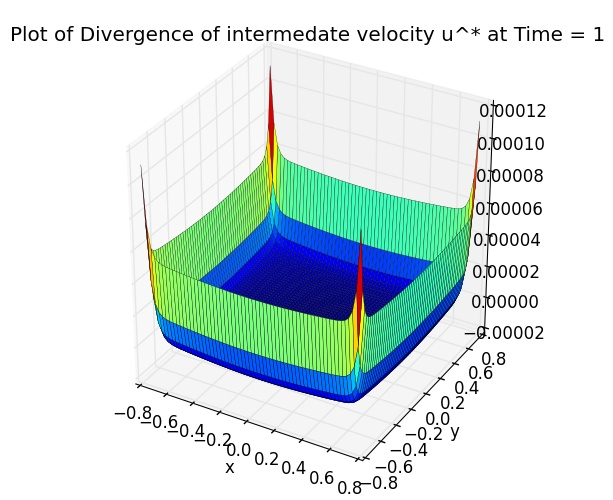
\includegraphics[width=2.6in]{figures/Pm1b_unf1_np_div_uvstar_t_1_grid_60.jpg}
		\caption{Divergence of intermediate velocity field Alg 2}\label{fig:6.19b}
	\end{subfigure}
	\quad
	\centering
	\begin{subfigure}[t]{2.2in}
		\centering
		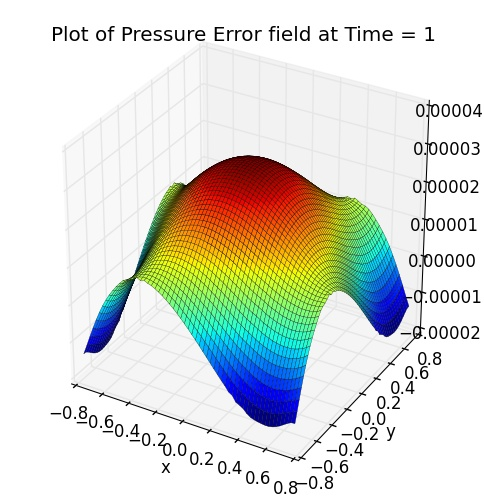
\includegraphics[width=2.2in]{figures/Pm2_unf1_np_P_error_t_1_grid_60.jpg}
		\caption{Pressure error field for Alg 3 method}\label{fig:6.19a}		
	\end{subfigure}
	\quad
	\begin{subfigure}[t]{2.5in}
		\centering
		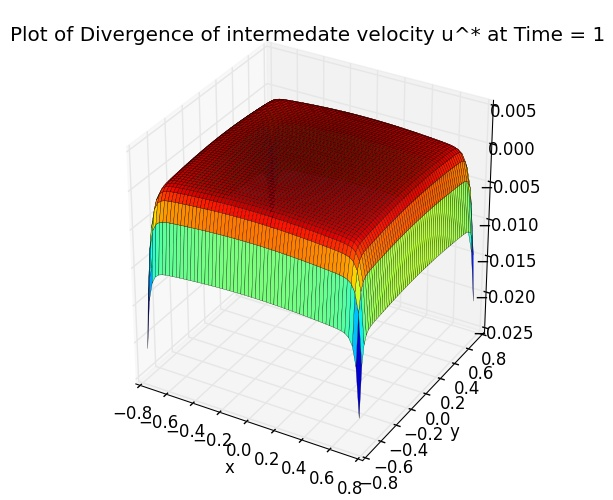
\includegraphics[width=2.5in]{figures/Pm2_unf1_np_div_uvstar_t_1_grid_60.jpg}
		\caption{Divergence of intermediate velocity field Alg 3}\label{fig:6.19b}
	\end{subfigure}
	\quad
	\begin{subfigure}[t]{2.5in}
		\centering
		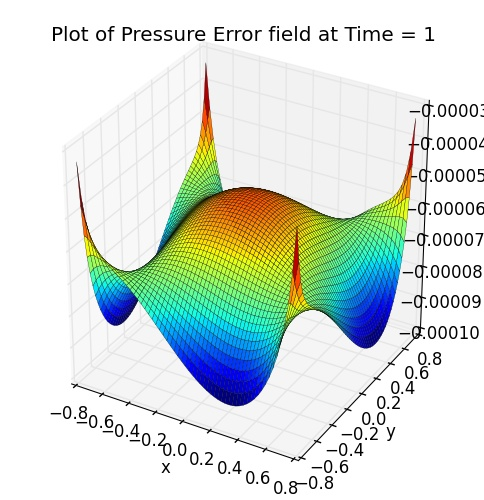
\includegraphics[width=2.5in]{figures/Gauge_unf1_P_error_t_1_grid_60.jpg}
		\caption{Pressure error field Gauge method }\label{fig:6.19b}
	\end{subfigure}
	\caption{Plot of Pressure error fields for the Unforced flow problem with Normalised Pressure approach used. Domain: $[-\dfrac{\pi}{4}, \dfrac{\pi}{4}]^2$, time = 1 and CFL = 0.5.}\label{fig:6.16}
\end{figure}

To further investigate the cause of degradation in accuracy in Alg 2, recall in normal mode analysis, we showed that the choice of pressure approximation $q = p^{n-1/2}$ results contradicting normal pressure gradient along the boundary especially if the normal analytic pressure gradient is not zero. This is the case in this unforced flow problem. For instance, the normal pressure gradient at west boundary ($x=\dfrac{\pi}{4}$ at any time is: $\dfrac{1}{2}\left(-\sin(\dfrac{\pi}{4}\right)$ which is obviously not zero. Hence this means this choice of $q$ does not work properly at the boundary.\\

It is supported by the plot of normal pressure gradient at West boundary. The plot of numerical solution is different to that of the analytical solution. This is amplified at the 4 corners of the domain where large spikes occur. We therefore infer that it is the non-smoothness caused by the inconsistent pressure approximation which degrades the global convergence of Alg 2.\\

We now propose a simplified modification to solve the problem by defining $q$ to be $q = 2\phi^{n-1/2} - \phi^{n-3/2}$. This results in a second order accurate pressure approximation to $p^{n+1/2}$. This can be shown using a simple Taylor series argument. With this modified pressure approximation $q$, the numerical normal pressure gradient now approximates the analytic one better. It is converging to the analytic pressure gradient at higher than second order rate too. The non-smooth spikes are now eliminated which reduces the error and also lifts up the global pressure error convergence to 2.5 order.

\begin{figure}[H]
	\centering
	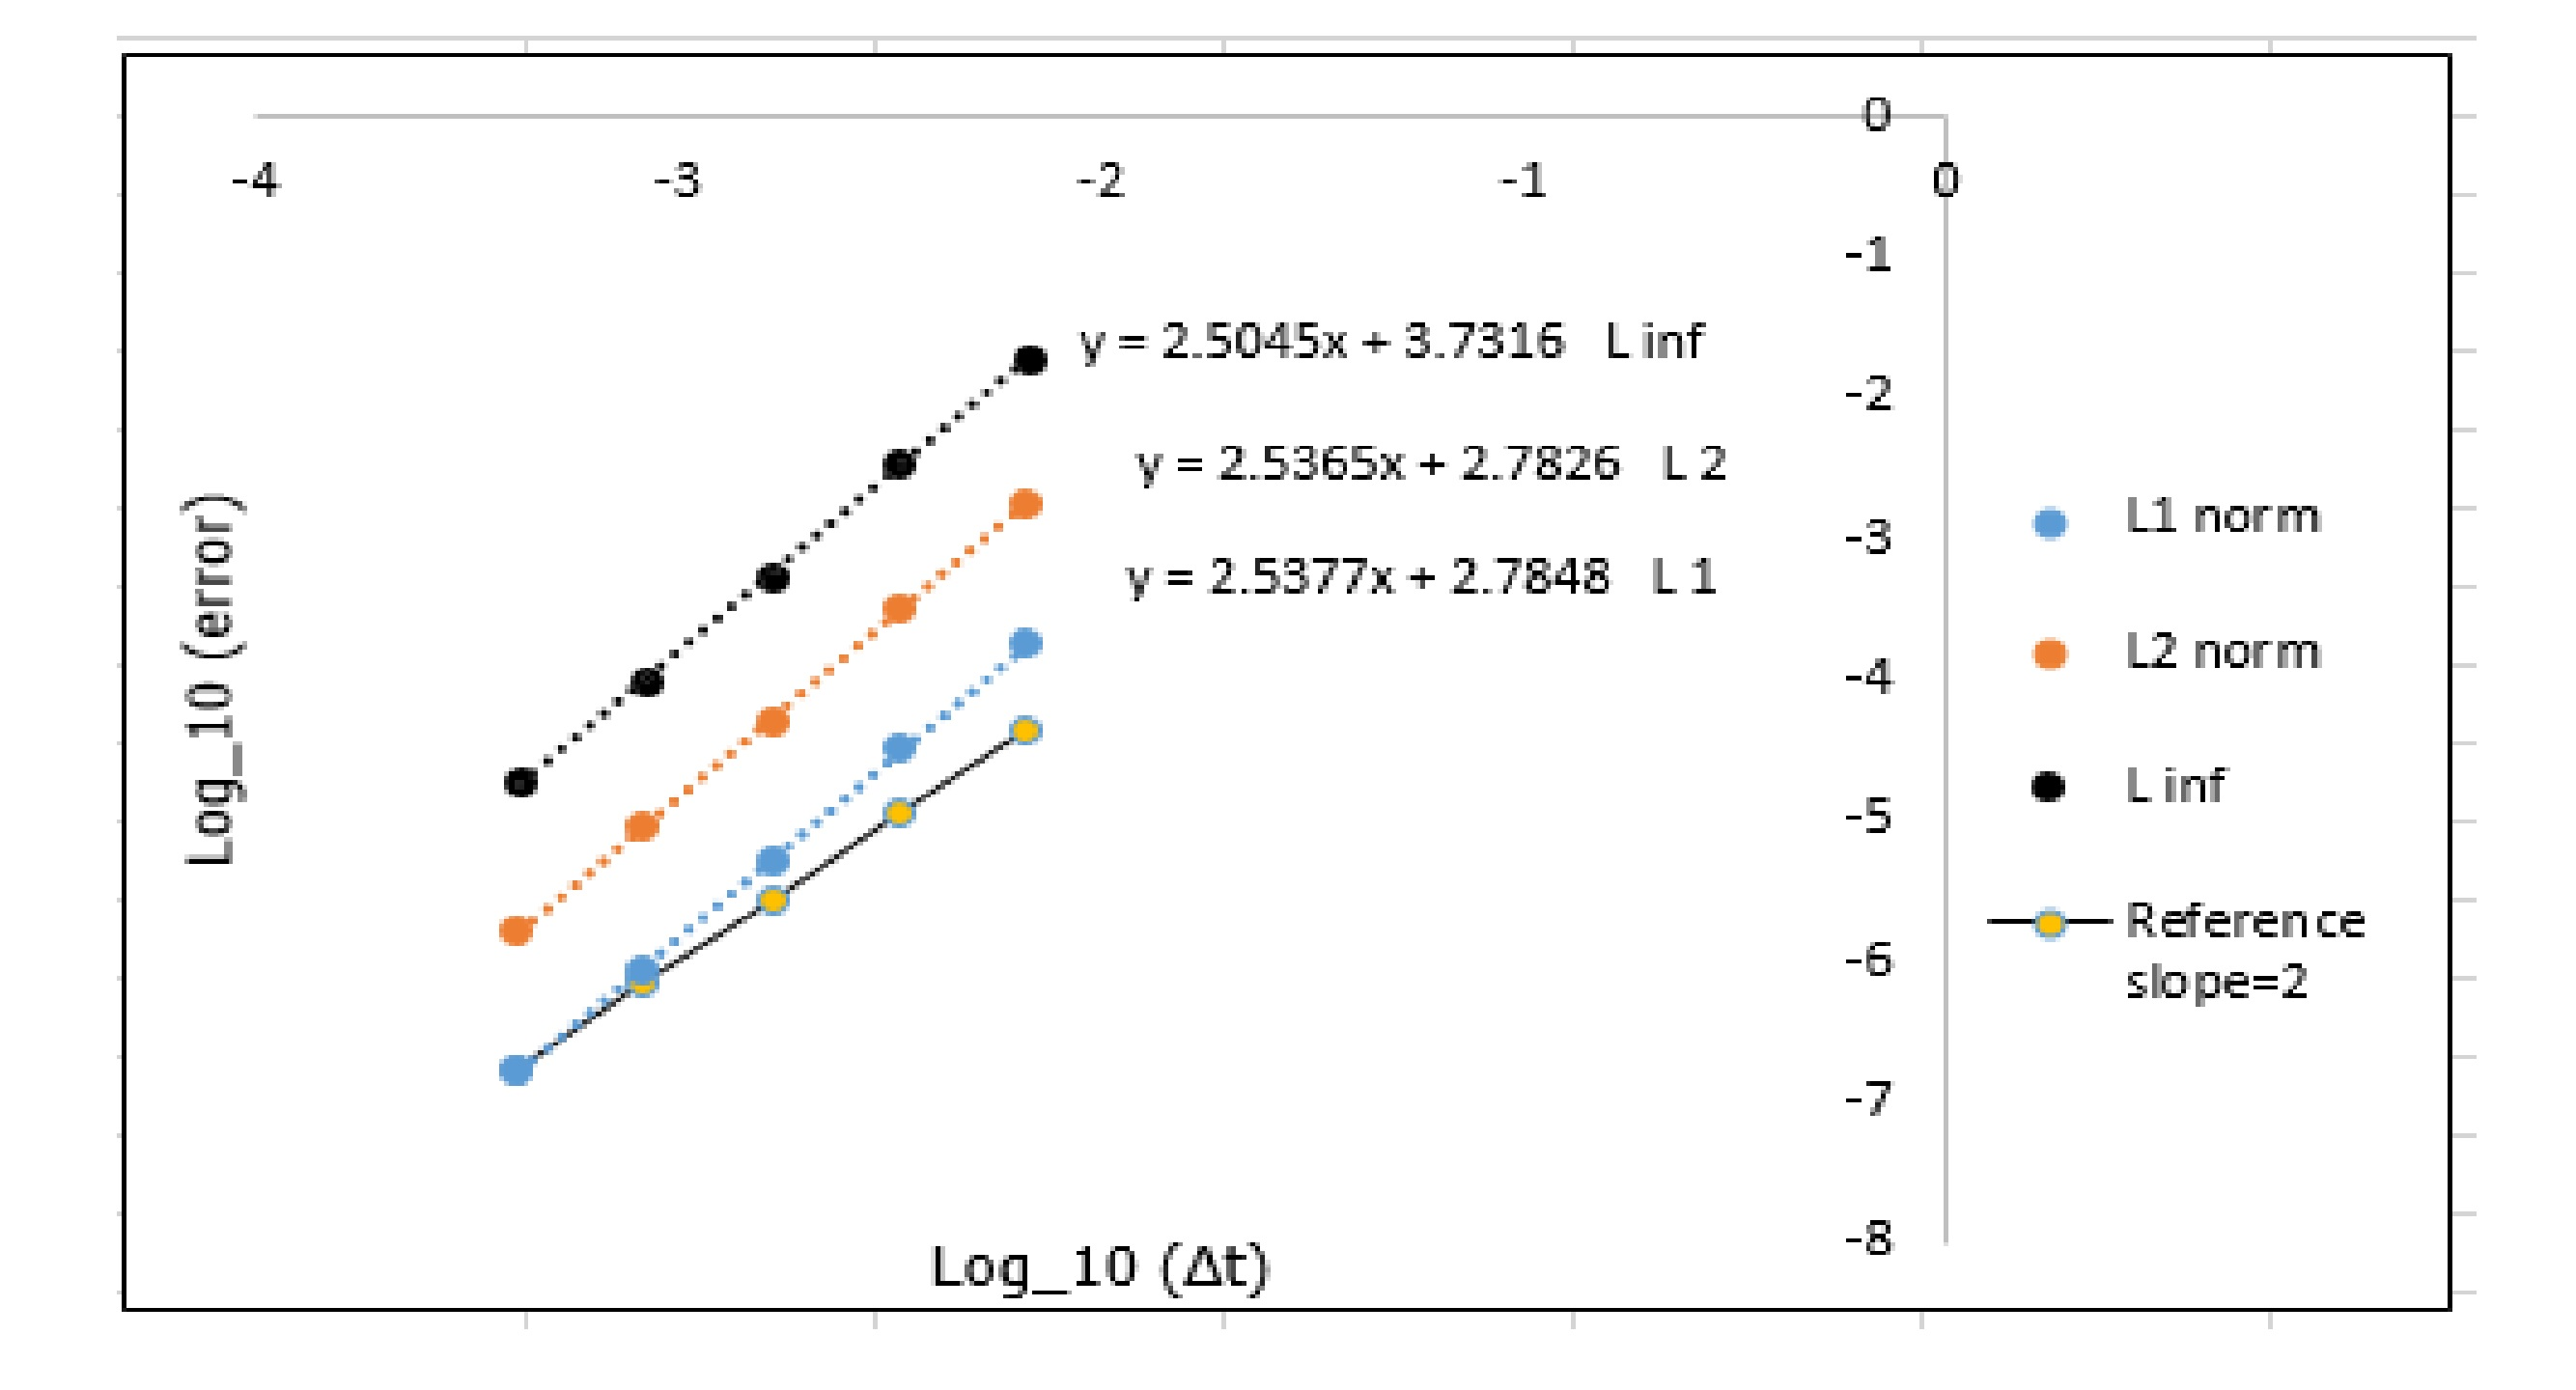
\includegraphics[width=4.5in]{figures/Pm1b2_unf1_np_P_rate.jpg}
	\caption{Log - log plot of the pressure error convergence rate with the modified $q = 2\phi^{n-1/2} - \phi^{n-3/2}$ used }\label{fig:6.23}
\end{figure}

\begin{figure}[H]
	\centering
	\begin{subfigure}[t]{2.6in}
		\centering
		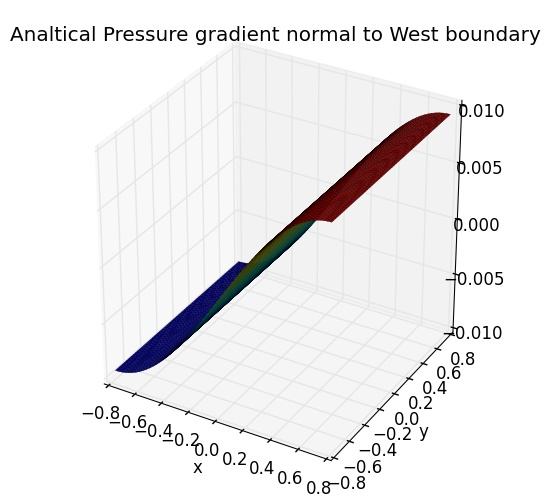
\includegraphics[width=2.6in]{figures/Pm1b2_unf1_np_W_NPexgrad_t_1_grid_60.jpg}
		\caption{Plot of analytic pressure gradient normal to west boundary}\label{fig:6.19a}		
	\end{subfigure}
	\quad
	\begin{subfigure}[t]{2.2in}
		\centering
		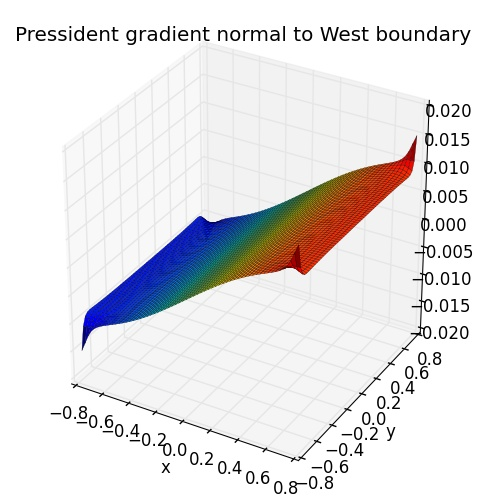
\includegraphics[width=2.2in]{figures/Pm1b_unf1_np_W_Npf_t_1_grid_60.jpg}
		\caption{Plot of numerical pressure gradient normal to west boundary with $q = p^{n-1/2}$ is used}\label{fig:6.19b}
	\end{subfigure}
	\quad
	\centering
	\begin{subfigure}[t]{2.5in}
		\centering
		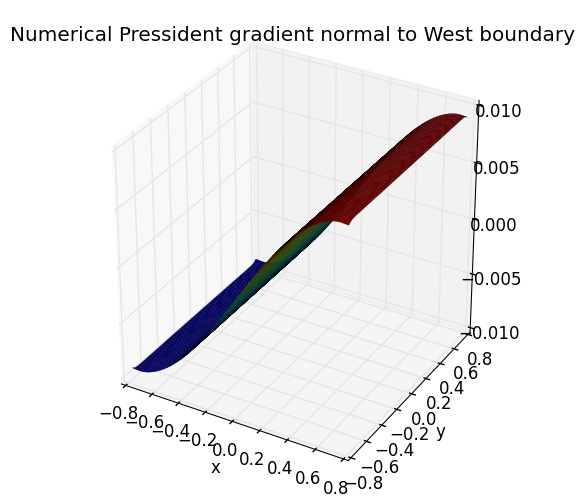
\includegraphics[width=2.5in]{figures/Pm1b2_unf1_np_W_Npf_t_1_grid_60.jpg}
		\caption{Plot of numerical pressure gradient normal to west boundary with the modified $q = 2\phi^{n-1/2} - \phi^{n-3/2}$ used}\label{fig:6.19a}		
	\end{subfigure}
	\caption{Plot of normal pressure gradients and convergence rates for Alg 2 with modified $q = 2\phi^{n-1/2} - \phi^{n-3/2}$ used. Domain: $[-\dfrac{\pi}{4}, \dfrac{\pi}{4}]^2$, time = 1 and CFL = 0.5.}\label{fig:6.16}
\end{figure}


\newpage
\section{Driven cavity flow}
In this section, we consider a very interesting flow problem: the Lid-Driven cavity. Driven cavity flow has been well studied in the literature. It is a simple example to show the effect of Reynolds number and turbulent and unsteady flows. We mainly illustrate the qualitative findings here through numerical simulations. There are however benchmark results for $3D$ and $2D$ Lid-driven cavity problems for the purpose of comparing accuracy of numerical solvers.\\ (\textbf{citation, Goda, Shen...})\\

Although the problem set up could vary, however the essential idea is the same. We have a fluid initially at rest except at one boundary where either horizontal or vertical component has a constant non-zero velocity (i.e. 1). The flow in the interior is then driven by the non-zero velocity at the boundary. This is like opening the lid along the non-zero boundary and sliding it at a constant velocity. The flow pattern depend on the value of Reynolds numbers and with low to moderate Reynolds number (often below 10000) the flow can reach to steady state whereas for higher Reynolds numbers, turbulence will occur in which no steady state solutions can be obtained. In fact, turbulence only occur in 3-dimensional type of flows and hence our $2D$ numerical solver would not show the pattern completely. Nevertheless, as our result presents, as Reynolds number increases, the flow does become unsteady which is aligned with the turbulence behaviour in $3D$ simulations.

\subsection{Problem set up}
We consider a fluid confined in the square domain: $[0,1]^2$. The fluid velocities are initially zero except for $v$ at the East boundary ($x=1$) which it is equal to 1 (i.e. $v(x=1,y,0)=1$). The problem set up is illustrated in the diagram below. The full Navier Stokes equations of incompressible flow is used. We consider the flow at different Reynolds numbers ($R = 1000, 10000$). The Gauge method was used to compute the solutions with grid size $100 \times 100$ and $CFL = 0.5$. \\

\begin{figure}[H]
	\centering
	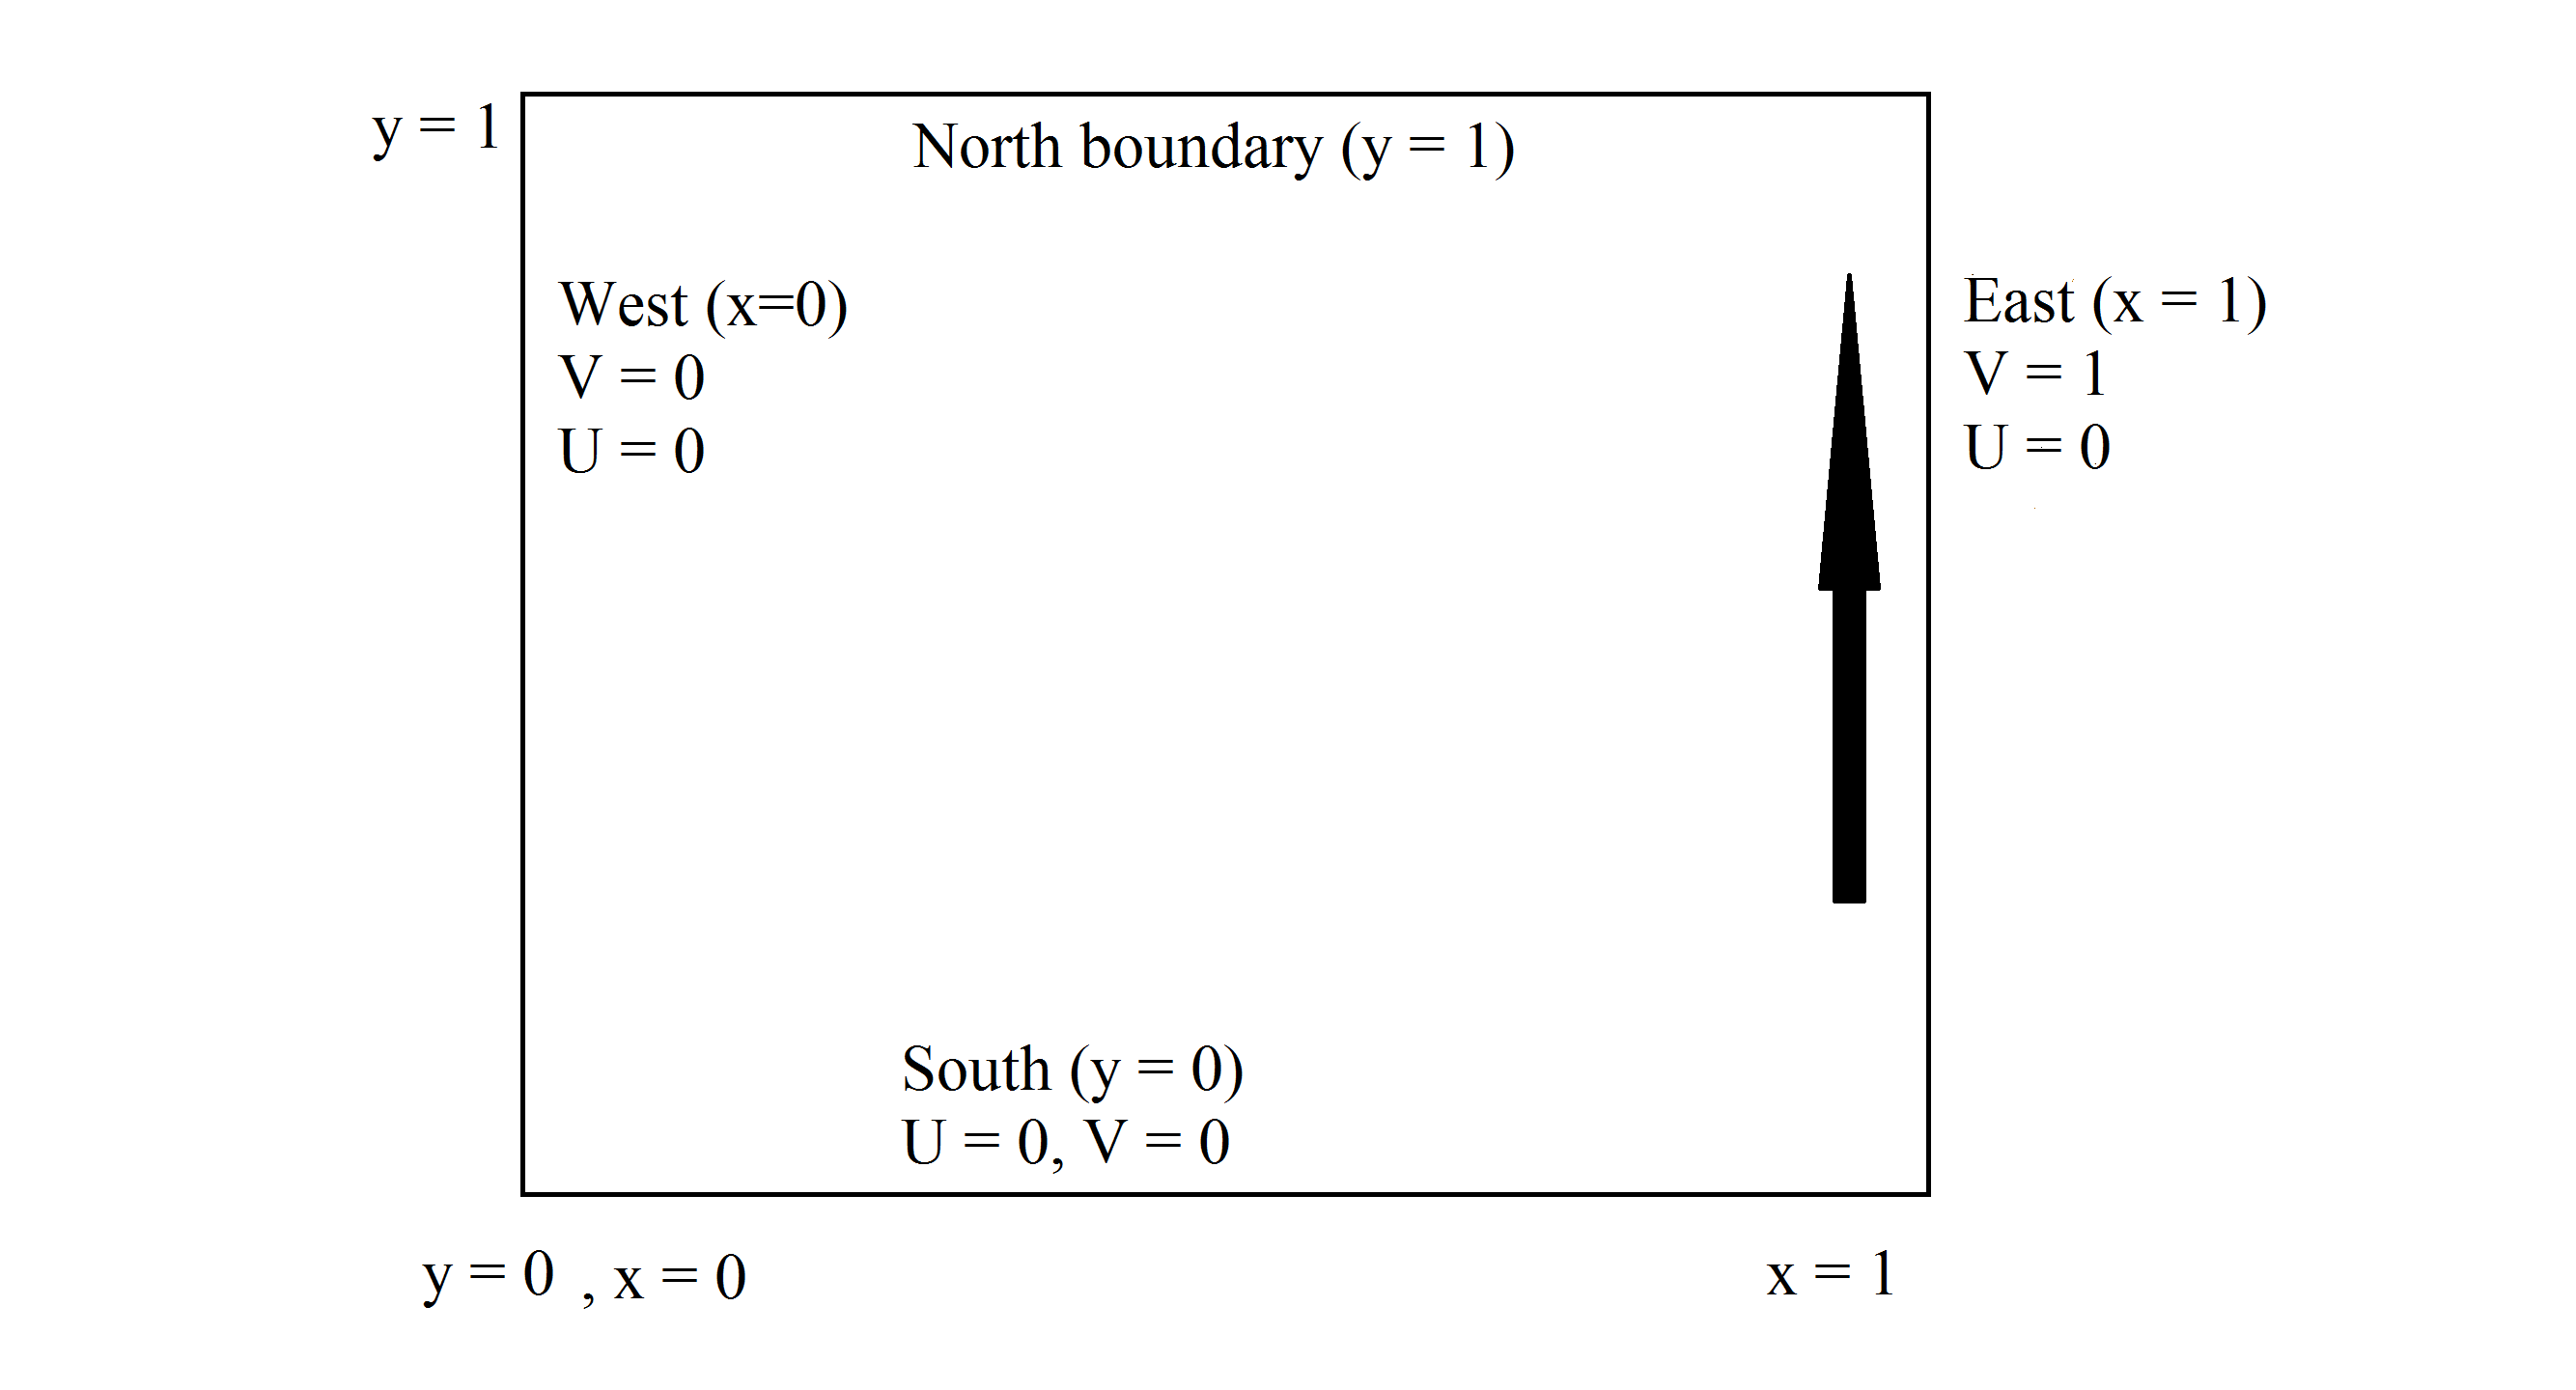
\includegraphics[width=5.5in]{figures/Lid_driven_set_up.png}
	\caption{Problem setup of the Lid-driven cavity. The flow is driven by the constant vertical velocity along the East boundary ($v=1$ at $x=1$)  }	
\label{fig:6.16}
\end{figure}
First we consider moderate Reynolds number flows of with value of 1000, the fluid converges to the steady state after about a time of 20s. 3 main eddies are formed. The main one starts from the corner near the East boundary since the initial flow starts from here. It then slides to the middle over time forming a constant main vortex. Mean while two other smaller eddies are then formed one after another. The streamline plots are presented below illustrate the flow patterns.\\

\subsection{Results}
At higher Reynolds number the flow become unsteady (or ``turbulent") as more smaller unsteady eddies are formed. This is clearly shown by the streamline plot at Reynold = 10000. Hence our result is in line with the literature too.\\

\begin{figure}[H]
	\centering
	\begin{subfigure}[t]{2.5in}
		\centering
		\includegraphics[width=2.5in]{figures/streamline_plot_t_0s_grid_100.pdf}
		\caption{Streamline plot of velocity fields at time 0s}\label{fig:6.19a}		
	\end{subfigure}
	\quad
	\begin{subfigure}[t]{2.5in}
		\centering
		\includegraphics[width=2.5in]{figures/streamline_plot_t_ 20s_grid_100.pdf}
		\caption{Streamline plot of velocity fields at time 20s}\label{fig:6.19b}
	\end{subfigure}
	\caption{Streamline plot of velocity fields for driven cavity flow. $v(x=1,y,t) = 1$ with grid size 100 and CFL = 0.5 used.}\label{fig:6.16}
\end{figure}

Reynolds number = 10000
\begin{figure}[H]
	\centering
	\includegraphics[width=3.0in]{figures/streamline_plot_t_20_grid30_Re_10000.pdf}
	\caption{Streamline plot of velocity fields at time 20s with Reynolds number equal to 10000}\label{fig:6.19}		
\label{fig:6.16}
\end{figure}

Plots of velocity and pressure solutions are also shown below:
\begin{figure}[H]
	\centering
	\begin{subfigure}[t]{2.5in}
		\centering
		\includegraphics[width=2.5in]{figures/Gauge_dcv_uf_grid_120.jpg}
		\caption{Plot of $U$ velocity at time 15s}\label{fig:6.19a}		
	\end{subfigure}
	\quad
	\begin{subfigure}[t]{2.5in}
		\centering
		\includegraphics[width=2.5in]{figures/Gauge_dcv_vf_grid_120.jpg}
		\caption{Plot of $V$ velocity at time 15s}\label{fig:6.19b}
	\end{subfigure}
	\quad
	\centering
	\begin{subfigure}[t]{3.5in}
		\centering
		\includegraphics[width=2.5in]{figures/Gauge_dcv_pf_grid_120.jpg}
		\caption{Plot of Pressure at time 15s}\label{fig:6.19a}		
	\end{subfigure}
	\caption{Plot of velocity and pressure solutions for driven cavity problem with Reynolds number equal to 1000. The East boundary for $V$ velocity is kept to be 1 over time. Grid size of 100 and CFL = 0.5 was used.}\label{fig:6.16}
\end{figure}

Although our result shows the unsteady pattern of flow as Reynolds number increases which is in line with the literature in general \textbf{Citation}, however to examine the turbulent behaviour we should implement $3D$ numerical solvers. This could be a further investigation in the future. Once again this section is only aimed to be a qualitative illustration of the classic Lid-driven cavity problem. 
